\documentclass[10pt,a4paper]{article}\usepackage[]{graphicx}\usepackage[]{color}
%% maxwidth is the original width if it is less than linewidth
%% otherwise use linewidth (to make sure the graphics do not exceed the margin)
\makeatletter
\def\maxwidth{ %
  \ifdim\Gin@nat@width>\linewidth
    \linewidth
  \else
    \Gin@nat@width
  \fi
}
\makeatother

\definecolor{fgcolor}{rgb}{0.345, 0.345, 0.345}
\newcommand{\hlnum}[1]{\textcolor[rgb]{0.686,0.059,0.569}{#1}}%
\newcommand{\hlstr}[1]{\textcolor[rgb]{0.192,0.494,0.8}{#1}}%
\newcommand{\hlcom}[1]{\textcolor[rgb]{0.678,0.584,0.686}{\textit{#1}}}%
\newcommand{\hlopt}[1]{\textcolor[rgb]{0,0,0}{#1}}%
\newcommand{\hlstd}[1]{\textcolor[rgb]{0.345,0.345,0.345}{#1}}%
\newcommand{\hlkwa}[1]{\textcolor[rgb]{0.161,0.373,0.58}{\textbf{#1}}}%
\newcommand{\hlkwb}[1]{\textcolor[rgb]{0.69,0.353,0.396}{#1}}%
\newcommand{\hlkwc}[1]{\textcolor[rgb]{0.333,0.667,0.333}{#1}}%
\newcommand{\hlkwd}[1]{\textcolor[rgb]{0.737,0.353,0.396}{\textbf{#1}}}%

\usepackage{framed}
\makeatletter
\newenvironment{kframe}{%
 \def\at@end@of@kframe{}%
 \ifinner\ifhmode%
  \def\at@end@of@kframe{\end{minipage}}%
  \begin{minipage}{\columnwidth}%
 \fi\fi%
 \def\FrameCommand##1{\hskip\@totalleftmargin \hskip-\fboxsep
 \colorbox{shadecolor}{##1}\hskip-\fboxsep
     % There is no \\@totalrightmargin, so:
     \hskip-\linewidth \hskip-\@totalleftmargin \hskip\columnwidth}%
 \MakeFramed {\advance\hsize-\width
   \@totalleftmargin\z@ \linewidth\hsize
   \@setminipage}}%
 {\par\unskip\endMakeFramed%
 \at@end@of@kframe}
\makeatother

\definecolor{shadecolor}{rgb}{.97, .97, .97}
\definecolor{messagecolor}{rgb}{0, 0, 0}
\definecolor{warningcolor}{rgb}{1, 0, 1}
\definecolor{errorcolor}{rgb}{1, 0, 0}
\newenvironment{knitrout}{}{} % an empty environment to be redefined in TeX

\usepackage{alltt}
\usepackage[utf8x]{inputenc}
\usepackage{amsmath}
\usepackage{amsfonts}
\usepackage{amssymb}
\usepackage{graphicx}
\usepackage{url}
\usepackage{fancyvrb}
\usepackage[unicode=true,pdfusetitle,
 bookmarks=true,bookmarksnumbered=true,bookmarksopen=true,bookmarksopenlevel=2,
 breaklinks=false,pdfborder={0 0 1},backref=false,colorlinks=false]
 {hyperref}
\hypersetup{
 pdfstartview={XYZ null null 1}}
\usepackage{breakurl}

\newcommand{\PE}{package \texttt{performanceEstimation}\ }

\author{Luis Torgo\\FCUP - LIAAD/INESC Tec\\University of Porto\\
  \texttt{ltorgo@dcc.fc.up.pt}, \texttt{ltorgo@inescporto.pt}}
\title{An Infra-Structure for Performance Estimation\\ and Experimental Comparison on Predictive Models}
\IfFileExists{upquote.sty}{\usepackage{upquote}}{}

\begin{document}



%$
\maketitle

\begin{abstract}
  
   This document describes an infra-structure provided by the package \PE that allows to estimate the performance of different approaches (workflows) to predictive tasks.  The infra-structure is generic in the sense that it can be used to estimate the values of any performance metrics, for any workflow on different predictive analytics tasks, namely, classification, regression and time series tasks. The package also includes several standard workflows that allow users to easily set up their experiments limiting the amount of work and information they need to give provide.
   
\end{abstract}

\section{Introduction}

The goal of this document is to describe the infra-structure that is available in package \PE to  estimate the performance of different approaches to predictive tasks.  The main goal of this package is to provide a general infra-structure that can be used to estimate the performance using several predictive performance metrics of any modelling approach to different predictive tasks, with a minimal effort from the user. The package provides this type of facilities for classification, regression and time series predictive tasks. There is no limitation on the type of approaches to these tasks for which you can estimate the performance - the user just needs to provide a workflow function (following some interface rules) that implements the approach for which the predictive performance is to be estimated. The package includes some standard workflow functions that implement the standard learn+test+evaluate approach that most users will be interested in. This means that if you just want to estimate the performance of some variants of a method already implemented in R (e.g. an SVM), on some particular tasks, you will be able to use these standard workflow functions and thus your input will be limited to the minimum. The package also provides a series of predictive performance metrics for different tasks. Still, you are not limited to these metrics and can use any metric provide it exists in R or you provide a function implementing it. 

This infra-structure implements different methods for estimating the predictive performance. Namely, you can select among:  (i) cross validation, (ii) holdout and random subsampling, (iii) leave one out cross validation, (iv) ($\epsilon_0$ and .631) bootstrap and also (v) Monte-Carlo experiments for time series forecasting tasks. For each of these tasks different options are implemented (e.g. use of stratified sampling).

Experimental methodologies for performance estimation are iterative
processes that repeat the modelling task several times using different
data samples with the goal of improving the accuracy of the
estimates. The estimates are the result of aggregating the scores
obtained on each of the repetitions. For each of these
repetitions different training and testing samples are generated and
the process being evaluated is "asked" to: (i) obtain the predictive
model using the training data, and then (ii) use this model to obtain
predictions for the respective test sample, which in turn (iii) can be
used to calculate the scores of the performance metrics being
estimated. This means that there is a workflow that starts with a
predictive task for which training and testing samples are given, and
that it should produce as result the scores of the performance metrics
being estimated. There are far too many possible approaches and
sub-steps for the implementation of this workflow.  To ensure full
generality of the infra-structure, we ask the user to provide a
function that implements this workflow for each of the predictive
approaches he/she wishes to compare and/or evaluate. This function can
be parametrizable in the sense that there may be variants of the
workflow that the user wishes to evaluate and/or compare. Still, the
goal of this workflow implementation functions is very clear: (i)
receive as input a predictive task for which training  and  test
samples are given, as well as any eventual workflow specific parameters; and
(ii) produce as result a set of scores for the evaluation metrics
being estimated. These scores should be obtained by applying some
modelling technique to the training sample and then use the resulting
to model to obtain predictions for the test sample. These predictions
should then be used to obtain the scores of the predictive metrics for which the
user is interested in obtaining reliable estimates.

The infra-structure we describe here provides means for the user to
indicate: (i) a set of predictive tasks with the respective data sets;
(ii) a set of workflows and respective variants; and (iii) an
experimental methodology. The infra-structure then takes care of all
the process of experimentally estimating the predictive performance of the different approaches on
the tasks, producing as result an object that can be
explored in different ways to obtain the results of the estimation process.
The infra-structure also provides several utility functions
to explore these results objects, for instance to
obtain summaries of the estimation process both in textual format as well as
visually. Moreover, it also provides functions that carry out
statistical significance tests based on the outcome of the
experiments. 

Finally, the infra-structure provides utility functions
implementing frequently used workflows for common modelling techniques, as
well as functions that facilitate the automatic generation of variants
of workflows by specifying sets of parameters that the user wishes to
consider in the comparisons.

\section{A Simple Illustrative Example}\label{sec:simpleEx}

Let us assume we are interested in comparing several variants of
an SVM on the
\textbf{Iris} classification problem. More specifically, we want to
obtain a reliable estimate of the error rate of these variants using
10-fold cross validation. The following code illustrates how these
estimates could be obtained with our proposed infra-structure.

\begin{knitrout}
\definecolor{shadecolor}{rgb}{0.969, 0.969, 0.969}\color{fgcolor}\begin{kframe}
\begin{alltt}
\hlkwd{library}\hlstd{(performanceEstimation)}
\hlkwd{library}\hlstd{(e1071)}
\hlkwd{data}\hlstd{(iris)}
\hlstd{res} \hlkwb{<-} \hlkwd{performanceEstimation}\hlstd{(}\hlkwd{PredTask}\hlstd{(Species} \hlopt{~} \hlstd{., iris),} \hlkwd{workflowVariants}\hlstd{(}\hlstr{"standardWF"}\hlstd{,} \hlkwc{learner} \hlstd{=} \hlstr{"svm"}\hlstd{,}
    \hlkwc{learner.pars} \hlstd{=} \hlkwd{list}\hlstd{(}\hlkwc{cost} \hlstd{=} \hlkwd{c}\hlstd{(}\hlnum{1}\hlstd{,} \hlnum{5}\hlstd{,} \hlnum{10}\hlstd{),} \hlkwc{gamma} \hlstd{=} \hlkwd{c}\hlstd{(}\hlnum{0.1}\hlstd{,} \hlnum{0.001}\hlstd{))),} \hlkwd{CvSettings}\hlstd{(}\hlkwc{nReps} \hlstd{=} \hlnum{1}\hlstd{,}
    \hlkwc{nFolds} \hlstd{=} \hlnum{10}\hlstd{))}
\end{alltt}
\end{kframe}
\end{knitrout}


This simple example illustrates several key concepts of our
infra-structure. First of all, we have the main function  -
\texttt{performanceEstimation()}, which is used to carry out
the estimation process. It has 3 arguments: (i) a vector of
predictive tasks (in the example a single one); (ii) a vector of workflows; and (iii) the
estimation settings. 

Predictive tasks are S4 objects of class
\textbf{PredTask}. This class, also defined in our infra-structure,
describes a predictive task by: (i) a formula; (ii) the source data
set (an R data frame); and (iii) an optional name of the task (a
string). 

Workflows are S4 objects of class \textbf{Workflow}, which are also
defined within the infra-structure. These objects include two pieces
of information: (i) the name of the function (a string) implementing the
workflow; and (ii) the list of parameters to this function. The
function will be called from within 
\texttt{performanceEstimation()}  with a formula in the first
argument, a training sample (a data frame) on the second argument, a
test sample (another data frame) on the third, and then all the parameters
the user specifies in the list of parameters used when creating the
\textbf{Workflow} object. This means that the object
\texttt{Workflow('svmTrial',pars=list(cost=10,gamma=0.5))}, if used in a
call to \texttt{performanceEstimation}, will 
 generate calls of the type
\texttt{svmTrial(\textit{someFormula}, \textit{someTrainingSample}, \textit{someTestSample}, cost=10,
  gamma=0.5)}. In the illustrative example with \textbf{Iris} we are using the function \texttt{workflowVariants()} from our package to automatically
generate a vector of \textbf{Workflow} objects. This function can be used
to generate different variants of a workflow function using all
combinations of parameters of the workflow. In the code
above the workflow function is \texttt{standardWF()} which is another
auxiliar function we provide. This function implements a typical
workflow for different modelling techniques that are indicated through
its parameter \texttt{learner}. Above we are using it to generate
variants of calls to the \texttt{svm()} function, which is an implementation of an SVM available in package \texttt{e1071}~\cite{}.  Later we will provide
more details on the \texttt{standardWF} function. For now we can think of the call
to the \texttt{workflowVariants()} function as generating the following vector:\linebreak
\begin{verbatim}
c(Workflow('standardWF',
          pars=list(learner='svm',
                    learner.pars=list(cost=1,gamma=0.1))
         ), 
  Workflow('standardWF',
          pars=list(learner='svm',
                    learner.pars=list(cost=5,gamma=0.1))
         ),
...
...
 ) 
\end{verbatim}
 
The workflow implemented through function \texttt{standardWF()} by
default calculates the error rate of the used modelling techniques if
handling classification tasks, though we will see later that we can
specify other metrics.

Finally, the third parameter of the function
\texttt{performanceEstimation()} specifies the estimation settings
to use in the process. It is an S4 object of class
\textbf{ExpSettings} that in effect is an union that includes among
others the S4 class \textbf{CvSettings}. Objects of this latter class
include information on the number of repetitions of the cross
validation process (in our example 1 single repetition, which is the
default), the number of folds (10 above, which is also the default),
the random number generator seed and a logical indicating whether stratified
samples should be used (defaulting to \texttt{FALSE}, i.e. no stratification).

The result of the call to \texttt{performanceEstimation()} is an S4
object of the class \textbf{ComparisonResults}. These objects tipically are not
 directly explored by the end-user so we ommit their
details here\footnote{Interested readers may have a look at the corresponding
  help page - \texttt{class?ComparisonResults} .}. There are several utility
functions that allow the users to explore the results of the
experimental comparisons. Here are a few illustrative examples:




\begin{knitrout}
\definecolor{shadecolor}{rgb}{0.969, 0.969, 0.969}\color{fgcolor}\begin{kframe}
\begin{alltt}
\hlkwd{summary}\hlstd{(res)}
\end{alltt}
\begin{verbatim}
## 
## == Summary of a  Cross Validation Performance Estimation Experiment ==
##  1 x 10 - Fold Cross Validation run with seed =  1234 
## 
## * Predictive Tasks ::  iris
## * Workflows  ::  svm.v1, svm.v2, svm.v3, svm.v4, svm.v5, svm.v6
## 
## * Summary of Experiment Results:
## 
## -> Datataset:  iris 
## 
## 	*Workflow: svm.v1 
##             err
## avg     0.04667
## std     0.05488
## min     0.00000
## max     0.13333
## invalid 0.00000
## 
## 	*Workflow: svm.v2 
##             err
## avg     0.04000
## std     0.04661
## min     0.00000
## max     0.13333
## invalid 0.00000
## 
## 	*Workflow: svm.v3 
##             err
## avg     0.04000
## std     0.04661
## min     0.00000
## max     0.13333
## invalid 0.00000
## 
## 	*Workflow: svm.v4 
##            err
## avg     0.6867
## std     0.2014
## min     0.3333
## max     0.9333
## invalid 0.0000
## 
## 	*Workflow: svm.v5 
##             err
## avg     0.15333
## std     0.11780
## min     0.06667
## max     0.46667
## invalid 0.00000
## 
## 	*Workflow: svm.v6 
##             err
## avg     0.10667
## std     0.06441
## min     0.00000
## max     0.20000
## invalid 0.00000
\end{verbatim}
\end{kframe}
\end{knitrout}


The generic function \texttt{summary} allows us to obtain the
estimated scores for each compared approach on each predictive
task. For each performance metric (in this case only the error rate),
the function shows the estimated average performance, the standard
error of this estimate as well as minimum and maximum scores on the
different iterations of the experimental comparison. Moreover,
information is also given on eventual failures on some of the
iterations.

The best scores for each predictive task and metric can be obtained as follows:

\begin{knitrout}
\definecolor{shadecolor}{rgb}{0.969, 0.969, 0.969}\color{fgcolor}\begin{kframe}
\begin{alltt}
\hlkwd{topPerformers}\hlstd{(res)}
\end{alltt}
\begin{verbatim}
## $iris
##     Workflow Estimate
## err   svm.v2     0.04
\end{verbatim}
\end{kframe}
\end{knitrout}


The generic function \texttt{plot} can be used to obtain a graphical
display of the distribution of performance metrics across the
different iterations of the estimation process using box-plots, as
show in Figure~\ref{fig:ex1Iris}. In this case we can observe that the
performance is constant on all variants (which could also be observed
in the output of \texttt{summary}), which indicates that the different
levels of pruning are having no effect for this simple predictive
task.

\begin{knitrout}
\definecolor{shadecolor}{rgb}{0.969, 0.969, 0.969}\color{fgcolor}\begin{kframe}
\begin{alltt}
\hlkwd{plot}\hlstd{(res)}
\end{alltt}
\end{kframe}\begin{figure}[]


{\centering 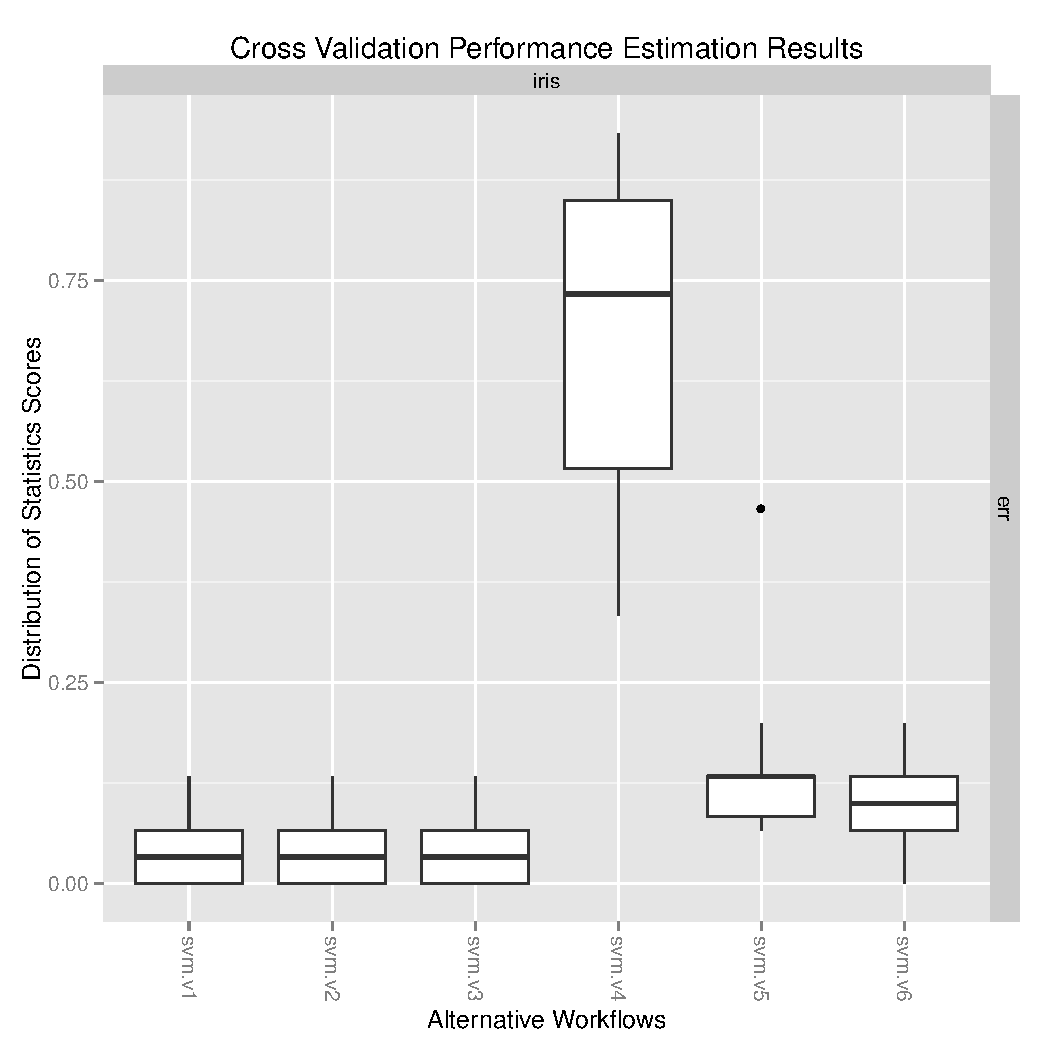
\includegraphics[width=0.7\textwidth]{figures/perfEst-ex1Iris} 

}

\caption[The distribution of the error rate on the 10 folds]{The distribution of the error rate on the 10 folds.\label{fig:ex1Iris}}
\end{figure}


\end{knitrout}


You might have observed that the infra-structure uses some IDs to
describe each workflow variant (e.g. \texttt{svm.v1}). The user can check
the parameter configuration corresponding to some ID as follows:

\begin{knitrout}
\definecolor{shadecolor}{rgb}{0.969, 0.969, 0.969}\color{fgcolor}\begin{kframe}
\begin{alltt}
\hlkwd{getWorkflow}\hlstd{(}\hlstr{"svm.v1"}\hlstd{, res)}
\end{alltt}
\begin{verbatim}
## Workflow Object:
## 	Workflow ID       ::  svm.v1 
## 	Workflow Function ::  standardWF
## 		Parameter values:
## 		 learner.pars  ->  cost=1 gamma=0.1 
## 		 learner  ->  svm
\end{verbatim}
\end{kframe}
\end{knitrout}


\section{Predictive Tasks}

Predictive tasks are data analysis problems where we want to obtain a
model of an unknown function $Y=f(X_1, X_2, \cdots, X_p)$ that relates
a target variable $Y$ with a set of $p$ predictors $X_1, X_2, \cdots,
X_p$. The model is usually obtained using a sample of $n$ observations
of the mapping of the unknown function, $D=\{\langle \mathbf{x}_i,
Y_i\rangle\}_{i=1}^n$, where $\mathbf{x}_i$ is a vector with the $p$
predictors values.  These data sets in R are usually stored in data
frames, and formula objects are used to specify the form of the
functional dependency that we are trying to model, i.e. which is the
target variable and the predictors.

Objects of class \textbf{PredTask} encapsulate the information of a
predictive task, i.e. the functional form and the data required for
solving it. For convenience they also allow the user to assign a name
to each task. These S4 objects can be created using the construtor
function \texttt{PredTask()}, as seen in the following example:

\begin{knitrout}
\definecolor{shadecolor}{rgb}{0.969, 0.969, 0.969}\color{fgcolor}\begin{kframe}
\begin{alltt}
\hlkwd{data}\hlstd{(iris)}
\hlkwd{PredTask}\hlstd{(Species} \hlopt{~} \hlstd{., iris,} \hlstr{"irisClassificationTask"}\hlstd{)}
\end{alltt}
\begin{verbatim}
## Prediction Task Object:
## 	Task Name ::  irisClassificationTask
## 	Formula   :: Species ~ .
## 	Task Data ::
## 'data.frame':	150 obs. of  5 variables:
##  $ Species     : Factor w/ 3 levels "setosa","versicolor",..: 1 1 1 1 1 1 1 1 1 1 ...
##  $ Sepal.Length: num  5.1 4.9 4.7 4.6 5 5.4 4.6 5 4.4 4.9 ...
##  $ Sepal.Width : num  3.5 3 3.2 3.1 3.6 3.9 3.4 3.4 2.9 3.1 ...
##  $ Petal.Length: num  1.4 1.4 1.3 1.5 1.4 1.7 1.4 1.5 1.4 1.5 ...
##  $ Petal.Width : num  0.2 0.2 0.2 0.2 0.2 0.4 0.3 0.2 0.2 0.1 ...
\end{verbatim}
\end{kframe}
\end{knitrout}


We should remark that the objects of this class only store the data
required for the specified task, as it should be clear from this other
simple example:

\begin{knitrout}
\definecolor{shadecolor}{rgb}{0.969, 0.969, 0.969}\color{fgcolor}\begin{kframe}
\begin{alltt}
\hlkwd{data}\hlstd{(iris)}
\hlkwd{PredTask}\hlstd{(Species} \hlopt{~} \hlstd{Petal.Length} \hlopt{+} \hlstd{Sepal.Length, iris,} \hlstr{"ShortIrisTask"}\hlstd{)}
\end{alltt}
\begin{verbatim}
## Prediction Task Object:
## 	Task Name ::  ShortIrisTask
## 	Formula   :: Species ~ Petal.Length + Sepal.Length
## 	Task Data ::
## 'data.frame':	150 obs. of  3 variables:
##  $ Species     : Factor w/ 3 levels "setosa","versicolor",..: 1 1 1 1 1 1 1 1 1 1 ...
##  $ Petal.Length: num  1.4 1.4 1.3 1.5 1.4 1.7 1.4 1.5 1.4 1.5 ...
##  $ Sepal.Length: num  5.1 4.9 4.7 4.6 5 5.4 4.6 5 4.4 4.9 ...
\end{verbatim}
\end{kframe}
\end{knitrout}


So, although we have supplied the full data frame to the constructor
function, as the task only uses 3 of the columns, the resulting
\textbf{PredTask} object only includes the information on the columns
required for this task.

\section{Workflows}

Estimation methodologies work most of the times by re-sampling the
available data set $D$ in order to create different train and test
samples from $D$ (an exception being a single repetition of Hold-out). The goal is to estimate the predictive performance
of a proposed workflow to solve the task, by using these different
samples to increase our confidence on the estimates. This workflow
consists on the process of obtaining a model from a given training
sample and then use it to obtain predictions for the given test
set. This process can include several steps, e.g. specific data
pre-processing steps, and may use any modelling approach, eventually
being proposed by the user. 

\subsection{User-defined Workflows}

With the goal of ensuring that the
proposed infra-structure is able to cope with all these possible usage
scenarios, we ask the user to take care of the writing of a function
implementing each workflow being compared/evaluated. These
user-defined workflow functions should be written assuming that the
first three arguments are: (i) the formula defining the predictive
task; (ii) the provided training sample; and (iii) the test sample
where to evaluate the obtained model. The functions may eventually
accept other arguments with specific parameters of the workflow. The
following is a general sketch of a user-defined workflow function:

\begin{Verbatim}
myWorkFlow <- function(form,train,test,..., .outPreds=TRUE, .outModel=TRUE) {
  require(mySpecialPackage,quietly=T)
  ## cary out some data pre-processing
  myTrain <- mySpecificPreProcessingSteps(train)
  ## now obtain the model
  myModel <- myModelingTechnique(form,myTrain,...)
  ## obtain the predictions
  preds <- predict(myModel,test)
  ## obtain the evaluation metric scores
  scores <- mySpecialEvaluationMetrics(responseValues(form,test),preds)
  ## finally produce the worflow output object
  res <- WFoutput(scores)
  if (.outPreds) workflowPredictions(res) <- list(responseValues(form,test),preds,rownames(test))
  if (.outModel) workflowInformation(res) <- list(model=myModel) 
  res
}
\end{Verbatim}

Not all workflows will require all these steps, though some may even
require more. This is clearly something that is up to the user. The
only strict requirements for these functions are: (i) the first 3 arguments
of the workflow function should be the formula, train and test data
frames; and (ii) the result of the function should be an object of the S4 class \textbf{WFoutput}.

Objects of class \textbf{WFoutput} contain the result of applying the workflow to a train+test partition. They are created using the constructor function \textbf{WFoutput()} that takes as argument a named vector with the scores of the metrics being estimated. These objects may optionally contain information on the true and predicted values for the target variable in the provided test set, as well as any other information the creator of the workflow function deems important to return. These two optional pieces of information are typically "attached" to the object using the replacement functions \textbf{workflowPredictions()}  and \textbf{workflowInformation()}, respectively. The \textbf{workflowPredictions()} function takes as value a list with at least two components. The first component is a vector with the true values of the target variable in the test set. The second component are the corresponding predictions made by the workflow. Finally, you may optionally provide a vector with the names of the rows in the test set. Regarding the \textbf{workflowInformation()} function it accepts as value also a list but whose content is completely free and left to the creator of the workflow function. Both these two functions can also be used to obtain the respective content from \textbf{WFoutput} objects, as we will see later in some of the illustrative examples.

The sketch shown above also illustrates the use of the function
\texttt{responseValues()} that can be used to obtain the values of the target
variable given a formula and a data frame.

Users should write one such workflow function for each process they
want to evaluate/compare. As mentioned before these functions may
accept further parameters on top of the 3 mandatory parameters. These
extra parameters will typically be parameters of the modelling
technique being used within the workflow but it is up to the user to
control this. As we have seen in Section~\ref{sec:simpleEx} we provide
the function \texttt{workflowVariants()} to facilitate the specification of
different variants of any workflow function by trying all combinations
of several of its specific parameters. For instance, if the modelling
function in the above example workflow (function
\texttt{myModelingTechnique()}) had an integer parameter \texttt{x}
and a Boolean parameter \texttt{y}, we could generate several
\textbf{Workflow} objects to be evaluated/compared using the
\texttt{performanceEstimation()} function, as follows:

\begin{knitrout}
\definecolor{shadecolor}{rgb}{0.969, 0.969, 0.969}\color{fgcolor}\begin{kframe}
\begin{alltt}
\hlkwd{workflowVariants}\hlstd{(}\hlstr{"myWorkFlow"}\hlstd{,} \hlkwc{x} \hlstd{=} \hlkwd{c}\hlstd{(}\hlnum{0}\hlstd{,} \hlnum{3}\hlstd{,} \hlnum{5}\hlstd{,} \hlnum{7}\hlstd{),} \hlkwc{y} \hlstd{=} \hlkwd{c}\hlstd{(T, F))}
\end{alltt}
\end{kframe}
\end{knitrout}


This would generate 8 variants of the same workflow with all
combinations of the specified values for the 2 parameters.  This means
that any parameter of the \texttt{workflowVariants()} function that has more
than one element is assumed to be a source for generation of
variants. There may be situations where this is not desirable, because
a particular argument of the workflow function is supposed to be a
vector. In these cases the user needs to ``tell'' the
\texttt{workflowVariants()} function that it should not generate variants from
the values of that parameter. Suppose that on the above example the
parameter \texttt{x} takes as values a vector, and thus your meaning
in the above statement is that you only have two variants of the
workflow (the different values of the parameter \texttt{y}). You could get
that effect by calling the \texttt{workflowVariants()} function as follows:

\begin{knitrout}
\definecolor{shadecolor}{rgb}{0.969, 0.969, 0.969}\color{fgcolor}\begin{kframe}
\begin{alltt}
\hlkwd{workflowVariants}\hlstd{(}\hlstr{"myWorkFlow"}\hlstd{,} \hlkwc{x} \hlstd{=} \hlkwd{c}\hlstd{(}\hlnum{0}\hlstd{,} \hlnum{3}\hlstd{,} \hlnum{5}\hlstd{,} \hlnum{7}\hlstd{),} \hlkwc{y} \hlstd{=} \hlkwd{c}\hlstd{(T, F),} \hlkwc{as.is} \hlstd{=} \hlkwd{c}\hlstd{(}\hlstr{"x"}\hlstd{))}
\end{alltt}
\end{kframe}
\end{knitrout}


While the previous call would generate 8 variants, this one only generates 2.

Let us see a concrete example of a user supplied workflow
function. Imagine we want to evaluate a kind of ensemble model formed
by a regression tree and a multiple linear regression model on an
algae blooms data set~\cite{Tor10}. Moreover, let us suppose we are
interested in using the correlation between the predictions and true
values as evaluation metric. We could start by writing the following
workflow function that implements our modelling approach:

\begin{knitrout}
\definecolor{shadecolor}{rgb}{0.969, 0.969, 0.969}\color{fgcolor}\begin{kframe}
\begin{alltt}
\hlstd{RLensemble} \hlkwb{<-} \hlkwa{function}\hlstd{(}\hlkwc{f}\hlstd{,} \hlkwc{tr}\hlstd{,} \hlkwc{ts}\hlstd{,} \hlkwc{weightRT} \hlstd{=} \hlnum{0.5}\hlstd{,} \hlkwc{step} \hlstd{=} \hlnum{FALSE}\hlstd{,} \hlkwc{...}\hlstd{) \{}
    \hlkwd{require}\hlstd{(DMwR,} \hlkwc{quietly} \hlstd{= F)}
    \hlstd{noNAsTR} \hlkwb{<-} \hlkwd{knnImputation}\hlstd{(tr)}
    \hlstd{noNAsTS} \hlkwb{<-} \hlkwd{knnImputation}\hlstd{(ts)}
    \hlstd{r} \hlkwb{<-} \hlkwd{rpartXse}\hlstd{(f, tr, ...)}
    \hlstd{l} \hlkwb{<-} \hlkwd{lm}\hlstd{(f, noNAsTR)}
    \hlkwa{if} \hlstd{(step)}
        \hlstd{l} \hlkwb{<-} \hlkwd{step}\hlstd{(l,} \hlkwc{trace} \hlstd{=} \hlnum{0}\hlstd{)}
    \hlstd{pr} \hlkwb{<-} \hlkwd{predict}\hlstd{(r, ts)}
    \hlstd{pl} \hlkwb{<-} \hlkwd{predict}\hlstd{(l, noNAsTS)}
    \hlstd{ps} \hlkwb{<-} \hlstd{weightRT} \hlopt{*} \hlstd{pr} \hlopt{+} \hlstd{(}\hlnum{1} \hlopt{-} \hlstd{weightRT)} \hlopt{*} \hlstd{pl}
    \hlkwd{c}\hlstd{(}\hlkwc{correlation} \hlstd{=} \hlkwd{cor}\hlstd{(}\hlkwd{resp}\hlstd{(f, ts), ps))}
\hlstd{\}}
\end{alltt}
\end{kframe}
\end{knitrout}


This workflow starts by building two modified samples of the training
and testing sets, with the \texttt{NA} values being filled in using a
nearest neighbour strategy (see the help page of the function
\texttt{knnImputation()} of package \textbf{DMwR}~\cite{Tor10} for more
details). These versions are to be used by the \texttt{lm()} function
that is unable to cope with cases with missing values. After obtaining
the two models and their predictions the function calculates a
weighted average of both predictions before obtaining and returning
the respective correlation score.

To evaluate different variants of this workflow we could run the
following experiment:

\begin{knitrout}
\definecolor{shadecolor}{rgb}{0.969, 0.969, 0.969}\color{fgcolor}\begin{kframe}
\begin{alltt}
\hlkwd{data}\hlstd{(algae,} \hlkwc{package} \hlstd{=} \hlstr{"DMwR"}\hlstd{)}
\hlstd{expRes} \hlkwb{<-} \hlkwd{performanceEstimation}\hlstd{(}\hlkwd{PredTask}\hlstd{(a1} \hlopt{~} \hlstd{., algae[,} \hlnum{1}\hlopt{:}\hlnum{12}\hlstd{],} \hlstr{"alga1"}\hlstd{),} \hlkwd{workflowVariants}\hlstd{(}\hlstr{"RLensemble"}\hlstd{,}
    \hlkwc{se} \hlstd{=} \hlkwd{c}\hlstd{(}\hlnum{0}\hlstd{,} \hlnum{1}\hlstd{),} \hlkwc{step} \hlstd{=} \hlkwd{c}\hlstd{(T, F),} \hlkwc{weightRT} \hlstd{=} \hlkwd{c}\hlstd{(}\hlnum{0.4}\hlstd{,} \hlnum{0.5}\hlstd{,} \hlnum{0.6}\hlstd{)),} \hlkwd{BootSettings}\hlstd{(}\hlkwc{nReps} \hlstd{=} \hlnum{100}\hlstd{,} \hlkwc{type} \hlstd{=} \hlstr{"e0"}\hlstd{))}
\end{alltt}
\end{kframe}
\end{knitrout}


In this experimental comparison we have used 100 repetitions of a $\epsilon_0$ 
bootstrap estimation procedure as estimation methodology (further
details on this and other methodologies will be given later), to
compare 12 variants of our workflow. 

\subsection{Generic Workflows}

Writing workflow functions may be tedious on large comparisons,
particularly when few details change among them. Moreover, the most
frequent use of our infra-structure will probably be to compare
existing modelling techniques on one or more problems. This means that
the most frequently used workflows will essentially build a model
using some existing algorithm, obtain its predictions and then
calculate some standard prediction error metrics. To facilitate this type of tasks, we
also provide generic workflow functions that carry out this type
of process for any modelling technique. The idea is to save the user
from having to write these functions provided his/her workflow fits
this generic schema.

\subsubsection{Classification and Regression Tasks}

Function \texttt{standardWF()} implements a typical workflow for both
classification and regression tasks. Apart from a formula, a training set data frame and a test set data frame, this function has the following parameters that help the user to specify is intended workflow:

\begin{description}
\item[learner] - the name of a R function that obtains a model from the training data. This function will be called with a formula in the first argument and the training set data frame in the second.
\item[learner.pars] - a list specifying any extra parameter settings that should be added to the formula and training set, at the time the learner function is called (defaults to \texttt{NULL}).
\item[predictor] - the name of a R function that is able to obtain the predictions of the model obtained with \texttt{learner}. This function will be called with the object resulting from the \texttt{learner} call on the first argument and the test set data frame in the second (it defaults to function \texttt{predict}).
\item[predictor.pars] - a list specifying any extra parameter settings that should be added to the model and test set, at the time the predictor function is called (defaults to \texttt{NULL}).
\item[evaluator] - the name of a R function that is able to calculate the evaluation metrics you want to estimate based on the predictions of the model and the true values of the target variable on the given test set (it will default to \texttt{classificationMetrics()} function if it is a classification task, and to \texttt{regressionMetrics()} if a regression task - check the respective help pages to see what are the default metrics that are calculated for each). This function will be called with the values of the target variable in the test set on the first argument and with the result of the call to the predictor function on the second.
\item[evaluator.pars] -  a list specifying any extra parameter settings that should be added to the true values and predictions, at the time the evaluator function is called (defaults to \texttt{NULL}). A typical usage here would be to use the parameter \texttt{stats} of functions \texttt{classificationMetrics()} and \texttt{regressionMetrics()} to specify the metrics you want to calculate, provided you are using these functions as evaluators.
\end{description}


Below you find an example of one of the most frequent type of
comparisons users carry out - checking which is the ``best'' model for
a given predictive task. Let us restrict the search to a small set of
models for illustrative purposes and let us play with the well-known
Boston housing regression task:

\begin{knitrout}
\definecolor{shadecolor}{rgb}{0.969, 0.969, 0.969}\color{fgcolor}\begin{kframe}
\begin{alltt}
\hlkwd{data}\hlstd{(Boston,} \hlkwc{package} \hlstd{=} \hlstr{"MASS"}\hlstd{)}
\hlkwd{library}\hlstd{(DMwR)}
\hlkwd{library}\hlstd{(e1071)}
\hlkwd{library}\hlstd{(randomForest)}
\hlstd{bostonRes} \hlkwb{<-} \hlkwd{performanceEstimation}\hlstd{(}\hlkwd{PredTask}\hlstd{(medv} \hlopt{~} \hlstd{., Boston),} \hlkwd{workflowVariants}\hlstd{(}\hlstr{"standardWF"}\hlstd{,}
    \hlkwc{learner} \hlstd{=} \hlkwd{c}\hlstd{(}\hlstr{"rpartXse"}\hlstd{,} \hlstr{"svm"}\hlstd{,} \hlstr{"randomForest"}\hlstd{)),} \hlkwd{CvSettings}\hlstd{(}\hlkwc{nReps} \hlstd{=} \hlnum{1}\hlstd{,} \hlkwc{nFolds} \hlstd{=} \hlnum{10}\hlstd{))}
\end{alltt}
\end{kframe}
\end{knitrout}


Notice that on this simple example we have used all modelling tools
with their default parameter settings which is not necessarily a good
idea when we are looking for the best performance. Still, the goal of
this illustration is to show you how simple this type of experiments
can be if you are using a standard workflow setting. In case you want
to use the modelling tools with other parameter settings then you
should separate them in different \texttt{workflowVariants()} calls, as shown
in the following example:

\begin{knitrout}
\definecolor{shadecolor}{rgb}{0.969, 0.969, 0.969}\color{fgcolor}\begin{kframe}
\begin{alltt}
\hlkwd{data}\hlstd{(Boston,} \hlkwc{package} \hlstd{=} \hlstr{"MASS"}\hlstd{)}
\hlkwd{library}\hlstd{(DMwR)}
\hlkwd{library}\hlstd{(e1071)}
\hlkwd{library}\hlstd{(randomForest)}
\hlstd{bostonRes} \hlkwb{<-} \hlkwd{performanceEstimation}\hlstd{(}\hlkwd{PredTask}\hlstd{(medv} \hlopt{~} \hlstd{., Boston),} \hlkwd{c}\hlstd{(}\hlkwd{workflowVariants}\hlstd{(}\hlstr{"standardWF"}\hlstd{,}
    \hlkwc{learner} \hlstd{=} \hlstr{"rpartXse"}\hlstd{,} \hlkwc{learner.pars} \hlstd{=} \hlkwd{list}\hlstd{(}\hlkwc{se} \hlstd{=} \hlkwd{c}\hlstd{(}\hlnum{0}\hlstd{,} \hlnum{1}\hlstd{))),} \hlkwd{workflowVariants}\hlstd{(}\hlstr{"standardWF"}\hlstd{,}
    \hlkwc{learner} \hlstd{=} \hlstr{"svm"}\hlstd{,} \hlkwc{learner.pars} \hlstd{=} \hlkwd{list}\hlstd{(}\hlkwc{cost} \hlstd{=} \hlkwd{c}\hlstd{(}\hlnum{1}\hlstd{,} \hlnum{5}\hlstd{),} \hlkwc{gamma} \hlstd{=} \hlkwd{c}\hlstd{(}\hlnum{0.01}\hlstd{,} \hlnum{0.1}\hlstd{))),} \hlkwd{workflowVariants}\hlstd{(}\hlstr{"standardWF"}\hlstd{,}
    \hlkwc{learner} \hlstd{=} \hlstr{"randomForest"}\hlstd{,} \hlkwc{learner.pars} \hlstd{=} \hlkwd{list}\hlstd{(}\hlkwc{ntree} \hlstd{=} \hlkwd{c}\hlstd{(}\hlnum{500}\hlstd{,} \hlnum{1000}\hlstd{)))),} \hlkwd{CvSettings}\hlstd{(}\hlkwc{nReps} \hlstd{=} \hlnum{1}\hlstd{,}
    \hlkwc{nFolds} \hlstd{=} \hlnum{10}\hlstd{))}
\end{alltt}
\end{kframe}
\end{knitrout}


Notice that this code involves estimating the mean squared error on the Boston Housing task for 8 different models through
10-fold cross validation. 


\subsubsection{Time Series Tasks}

Our infra-structure also includes another generic workflow function
that is specific for predictive tasks with time-dependent data
(e.g. time series forecasting problems). This workflow function
implements two different approaches to the problem of training a
 model with a set of time-dependent data and then use it to
obtain predictions for a test set in the future. These two approaches
contrast with the standard approach of learning a model with the
available training sample and then use it to obtain predictions for
all test period. This standard approach could be used with the previously
described \texttt{standardWF()} function. However, there are
alternatives to this procedure, two of the most common being the
sliding and growing window approaches, which are implemented in another workflow function developed for time series tasks.

Predictive tasks for time-dependent data are different from standard
classification and regression tasks because they require that the test
samples have time stamps that are more recent then training
samples. In this context, experimental methodologies handling these
tasks typically do not shuffle the observations to maintain the time ordering
in the original data. The most common setup is that we have a $L$ time steps
training window containing samples in the period $[t_1,t_L]$ and a $F$
time steps test window typically containing the observations in the
time window $[t_{L+1},t_{L+F}]$. In this context, the idea of the
sliding window method is that if we want a prediction for time point
$t_k$ belonging to the test interval $[t_{L+1},t_{L+F}]$ then we can
assume that all data from $t_{L+1}$ till $t_{k-1}$ is already past,
and thus usable by the model. In this context, it may be wise to use
this new data in the interval $[t_{L+1},t_{k-1}]$ to update the
original model obtained using only the initial training period data. This is
particularly advisable if we suspect that the conditions may have
changed since the training period has ended. Model updating using the
sliding window method is carried out by using the data in the $L$ last
time steps, i.e. every new model is always obtained using the last $L$
data observations, as if the training window was slided forward in
time. Our \texttt{timeseriesWF()} function implements this idea for
both time series with a numeric target variable and a nominal target
variable. This function has a parameter (\texttt{type}) that if set to
``slide'' will use a sliding window approach. As with the
\texttt{standardWF()} function, this \texttt{timeseriesWF()} function
also accepts parameters specifying the learner, predictor, evaluator
and their respective parameters. Moreover, this function also includes
an extra parameter, named \texttt{relearn.step}, which allows the user
to establish the frequency of model updating. By default this is every
new test sample, i.e. $1$, but the user may set a less frequent
model-updating policy by using higher values of this parameter.  The
idea of the growing window approach is very similar. The only difference
is on the data used when updating the models. Whilst sliding window
uses the data occurring in the last $L$ time steps, growing window
keeps increasing the original training window with the newly available
data points, i.e. the models are obtained with increasingly larger
training samples. By setting the parameter \texttt{type} to ``grow''
you get the \texttt{timseriesWF()} function to use this method.


\section{Estimation Methodologies}\label{sec:expMeth}

There are different ways of providing reliable estimates of the
predictive performance of a workflow. Our infra-structure implements some
of the most common estimation methods. In this section we
briefly describe them and provide short illustrative examples of their
use.

\subsection{Cross Validation}

$k$-Fold cross validation (CV) is one of the most common 
methods to estimate the predictive performance of a model. By
including an S4 object of class \textbf{CvSettings} in the third
argument of function \texttt{performanceEstimation()} we can carry
out experiments of this type.

The function \texttt{CvSettings()} can be used as a constructor of objects
of class \textbf{CvSettings}. It accepts the following parameters:

\begin{description}
\item[nReps] - the number of repetitions of the $k$-fold CV experiment (default is $1$)
\item[nFolds] - the number of $k$ folds to use (default is $10$)
\item[seed] - the random number generator seed to use (default is $1234$)
\item[strat] - whether to use stratified samples (default is \texttt{FALSE})
\item[dataSplits] - a list containing user-supplied data splits
  for each of the folds and repetitions (check the help page of the
  class for further details). This parameter defaults to
  \texttt{NULL}, i.e. no user-supplied splits, they are decided
  internally by the infra-structure.
\end{description}

Bellow you can find a small illustration using the Breast Cancer data
set available in package \textbf{mlbench}. On this example we compare
some variants of an SVM using a $3\times 10-$fold cross validation
process with stratified sampling because one of the two classes has a
considerably lower frequency.

\begin{knitrout}
\definecolor{shadecolor}{rgb}{0.969, 0.969, 0.969}\color{fgcolor}\begin{kframe}
\begin{alltt}
\hlkwd{data}\hlstd{(BreastCancer,} \hlkwc{package} \hlstd{=} \hlstr{"mlbench"}\hlstd{)}
\hlkwd{library}\hlstd{(e1071)}
\hlstd{bc} \hlkwb{<-} \hlkwd{knnImputation}\hlstd{(BreastCancer[,} \hlopt{-}\hlnum{1}\hlstd{])}
\hlstd{bcExp} \hlkwb{<-} \hlkwd{performanceEstimation}\hlstd{(}\hlkwd{PredTask}\hlstd{(Class} \hlopt{~} \hlstd{., bc,} \hlstr{"BreastCancer"}\hlstd{),} \hlkwd{workflowVariants}\hlstd{(}\hlstr{"standardWF"}\hlstd{,}
    \hlkwc{learner} \hlstd{=} \hlstr{"svm"}\hlstd{,} \hlkwc{learner.pars} \hlstd{=} \hlkwd{list}\hlstd{(}\hlkwc{cost} \hlstd{=} \hlkwd{c}\hlstd{(}\hlnum{1}\hlstd{,} \hlnum{5}\hlstd{),} \hlkwc{gamma} \hlstd{=} \hlkwd{c}\hlstd{(}\hlnum{0.01}\hlstd{,} \hlnum{0.1}\hlstd{)),} \hlkwc{evaluator.pars} \hlstd{=} \hlkwd{list}\hlstd{(}\hlkwc{stats} \hlstd{=} \hlkwd{c}\hlstd{(}\hlstr{"F"}\hlstd{,}
        \hlstr{"prec"}\hlstd{,} \hlstr{"rec"}\hlstd{),} \hlkwc{posClass} \hlstd{=} \hlstr{"malignant"}\hlstd{)),} \hlkwd{CvSettings}\hlstd{(}\hlkwc{nReps} \hlstd{=} \hlnum{3}\hlstd{,} \hlkwc{nFolds} \hlstd{=} \hlnum{10}\hlstd{,} \hlkwc{strat} \hlstd{=} \hlnum{TRUE}\hlstd{))}
\end{alltt}
\end{kframe}
\end{knitrout}


Please note the use of the \texttt{evaluator.pars} parameter of the \texttt{standardWF()} function. We have used it to indicate several settings to be used in the call to the evaluation function, which by default is \texttt{classificationMetrics} in the case of classification problems when using our standard workflow. In this case we are specifying some of the available classification metrics and indicating which of the two classes of the problem is to be considered the positive class\footnote{The F-measure, Recall and Precision metrics are calculated for two-class problems with respect to one of the classes, usually named the ``positive'' class.}

\subsection{Bootstrapping}

Bootstrapping or bootstrap resampling is another well-known
experimental methodology that is implemented in our
infra-structure. Namely, we implement two of the most common methods of obtaining bootstrap estimates: $\epsilon_0$ and $.632$ bootstrap.
By including an S4 object of class
\textbf{BootSettings} in the third argument of function
\texttt{performanceEstimation()} we can carry out experiments of this
type.

Function \texttt{BootSettings()} can be used as a constructor of
objects of class \textbf{BootSettings}. It accepts the following
arguments:

\begin{description}
\item[type] - a string with the type of bootstrap estimates: either "e0" for $\epsilon_0$ bootstrap, or ".632" for $.632$ bootstrap (default is "e0")
\item[nReps] - the number of repetitions of the bootstrap experiment (default is $200$)
\item[seed] - the random number generator seed to use (default is $1234$)
\item[dataSplits] - a list containing user-supplied data splits
  for each of the repetitions (check the help page of the
  class for further details). This parameter defaults to
  \texttt{NULL}, i.e. no user-supplied splits, they are decided
  internally by the infra-structure.
\end{description}

Bellow you can find a small illustration using the Servo data set available in package \textbf{mlbench}. On this example we compare some variants of an artificial neural network using 100 repetitions of a bootstrap experiment. 

\begin{knitrout}
\definecolor{shadecolor}{rgb}{0.969, 0.969, 0.969}\color{fgcolor}\begin{kframe}
\begin{alltt}
\hlkwd{data}\hlstd{(Servo,} \hlkwc{package} \hlstd{=} \hlstr{"mlbench"}\hlstd{)}
\hlkwd{library}\hlstd{(nnet)}
\hlstd{nnExp} \hlkwb{<-} \hlkwd{performanceEstimation}\hlstd{(}\hlkwd{PredTask}\hlstd{(Class} \hlopt{~} \hlstd{., Servo),} \hlkwd{workflowVariants}\hlstd{(}\hlstr{"standardWF"}\hlstd{,} \hlkwc{learner} \hlstd{=} \hlstr{"nnet"}\hlstd{,}
    \hlkwc{learner.pars} \hlstd{=} \hlkwd{list}\hlstd{(}\hlkwc{trace} \hlstd{= F,} \hlkwc{linout} \hlstd{= T,} \hlkwc{size} \hlstd{=} \hlkwd{c}\hlstd{(}\hlnum{3}\hlstd{,} \hlnum{5}\hlstd{),} \hlkwc{decay} \hlstd{=} \hlkwd{c}\hlstd{(}\hlnum{0.01}\hlstd{,} \hlnum{0.1}\hlstd{))),} \hlkwd{BootSettings}\hlstd{(}\hlkwc{nReps} \hlstd{=} \hlnum{100}\hlstd{))}
\end{alltt}
\end{kframe}
\end{knitrout}


\subsection{Holdout and Random Subsampling}

The Holdout is another frequently used experimental methodology,
particularly for large data sets. To carry out this type of
experiments in our infra-structure we can include an S4 object of
class \textbf{HldSettings} in the third argument of function
\texttt{performanceEstimation()}.

Function \texttt{HldSettings()} can be used as a constructor of
objects of class \textbf{HldSettings}. It accepts the following
arguments:

\begin{description}
\item[nReps] - the number of repetitions of the Holdout experiment (default is $1$)
\item[hldSz] - the percentage  of cases (a number between 0 and 1) to leave as holdout (test set) (default is $0.3$)
\item[seed] - the random number generator seed to use (default is $1234$)
\item[strat] - whether to use stratified samples (default is \texttt{FALSE})
\item[dataSplits] - a list containing user-supplied data splits
  for each of the repetitions (check the help page of the
  class for further details). This parameter defaults to
  \texttt{NULL}, i.e. no user-supplied splits, they are decided
  internally by the infra-structure.
\end{description}

Please note that for the usual meaning of Holdout the number of repetitions should be 1 (the default), while larger values of this parameter correspond to what is usually known as random subsampling.

The following is a small illustrative example of the use of the
random subsampling with the LetterRecognition classification task from package
\textbf{mlbench}.

\begin{knitrout}
\definecolor{shadecolor}{rgb}{0.969, 0.969, 0.969}\color{fgcolor}\begin{kframe}
\begin{alltt}
\hlkwd{data}\hlstd{(LetterRecognition,} \hlkwc{package} \hlstd{=} \hlstr{"mlbench"}\hlstd{)}
\hlstd{ltrExp} \hlkwb{<-} \hlkwd{performanceEstimation}\hlstd{(}\hlkwd{PredTask}\hlstd{(lettr} \hlopt{~} \hlstd{., LetterRecognition),} \hlkwd{workflowVariants}\hlstd{(}\hlstr{"standardWF"}\hlstd{,}
    \hlkwc{learner} \hlstd{=} \hlstr{"rpartXse"}\hlstd{,} \hlkwc{learner.pars} \hlstd{=} \hlkwd{list}\hlstd{(}\hlkwc{se} \hlstd{=} \hlkwd{c}\hlstd{(}\hlnum{0}\hlstd{,} \hlnum{1}\hlstd{)),} \hlkwc{predictor.pars} \hlstd{=} \hlkwd{list}\hlstd{(}\hlkwc{type} \hlstd{=} \hlstr{"class"}\hlstd{)),}
    \hlkwd{HldSettings}\hlstd{(}\hlkwc{nReps} \hlstd{=} \hlnum{3}\hlstd{,} \hlkwc{hldSz} \hlstd{=} \hlnum{0.3}\hlstd{))}
\end{alltt}
\end{kframe}
\end{knitrout}


Please note the use of the \texttt{predictor.pars} parameter of our \texttt{standardWF()} function to be able to cope with the fact that the \texttt{predict} method for classification trees requires the use of \texttt{type="class"} to get actual predicted class labels instead of class probabilities.

\subsection{Leave One Out Cross Validation}

Leave one out cross validation is a type of cross validation method
that is mostly used for small data sets. You can think of leave one
out cross validation as a $k$-fold cross validation with $k$ equal to
the size of the available data set. To carry out this type of
experiments in our infra-structure we can include an S4 object of
class \textbf{LoocvSettings} in the third argument of function
\texttt{performanceEstimation()}.

Function \texttt{LoocvSettings()} can be used as a constructor of
objects of class \textbf{LoocvSettings}. It accepts the following
arguments:

\begin{description}
\item[seed] - the random number generator seed to use (default is $1234$)
\item[verbose] - whether the execution of the experiments should provide a verbose form of output (default is \texttt{FALSE})
\end{description}


The following is a small illustrative example of the use of the
Holdout with the LetterRecognition classification task from package
\textbf{mlbench}.

\begin{knitrout}
\definecolor{shadecolor}{rgb}{0.969, 0.969, 0.969}\color{fgcolor}\begin{kframe}
\begin{alltt}
\hlkwd{data}\hlstd{(iris)}
\hlkwd{library}\hlstd{(e1071)}
\hlstd{irisExp} \hlkwb{<-} \hlkwd{performanceEstimation}\hlstd{(}\hlkwd{PredTask}\hlstd{(Species} \hlopt{~} \hlstd{., iris),} \hlkwd{workflowVariants}\hlstd{(}\hlstr{"standardWF"}\hlstd{,}
    \hlkwc{learner} \hlstd{=} \hlstr{"svm"}\hlstd{,} \hlkwc{learner.pars} \hlstd{=} \hlkwd{list}\hlstd{(}\hlkwc{cost} \hlstd{=} \hlkwd{c}\hlstd{(}\hlnum{1}\hlstd{,} \hlnum{10}\hlstd{))),} \hlkwd{LoocvSettings}\hlstd{())}
\end{alltt}
\end{kframe}
\end{knitrout}



\subsection{Monte Carlo Experiments}

Monte Carlo experiments are similar to random subsampling (or repeated
Holdout) in the sense that they consist of repeating a learning +
testing cycle several times using different data samples. The main
different lies on the way the samples are obtained. In Monte Carlo
experiments the original order of the observations is respected and
train and test splits are obtained such that the testing samples
appear ``after'' the training samples, thus being the methodology of
choice when you are comparing time series forecasting models. The idea
of Monte Carlo experiments is the following: (i) given a data set
spanning from time $t_1$ till time $t_N$, (ii) given a training set
time interval size $L$ and a test set time interval size $F$, such
that $T+F < N$, (iii) Monte Carlo experiments generate $R$ random time
points from the interval $[t_{1+T},t_{N-F}]$, and then (iv) for each
of these $R$ time points they generate a training set with data in the
interval $[t_{R-T+1},t_{R}]$ and a test set with data in the interval
$[t_{R+1},t_{R+F}]$. Using this process $R$ train+test cycles are
carried out using the user-supplied workflow function, and the
experiment estimates result from the average of the $R$ scores as
usual.

To carry out this type of experiments in our infra-structure we can
include an S4 object of class \textbf{McSettings} in the third
argument of function \texttt{performanceEstimation()}.

The function \texttt{McSettings()} can be used as a constructor of
objects of class \textbf{McSettings}. It accepts the following
arguments:

\begin{description}
\item[nReps] - the number of repetitions of the Monte Carlo experiment (default is $10$)
\item[szTrain] - the percentage (a number between 0 and 1) or the actual number of cases to use in the training samples (default is $0.25$)
\item[szTest] - the percentage (a number between 0 and 1) or the actual  number of cases to use in the test samples (default is $0.25$)
\item[seed] - the random number generator seed to use (default is $1234$)
\item[dataSplits] - a list containing user-supplied data splits
  for each of the repetitions (check the help page of the
  class for further details). This parameter defaults to
  \texttt{NULL}, i.e. no user-supplied splits, they are decided
  internally by the infra-structure.
\end{description}

The following is a small illustrative example using the quotes of the
SP500 index. This example compares two random forests with 500
regression trees, one applied in a standard way, and the other using
a sliding window with a relearn step of 5 days. The experiment
uses 10 repetitions of a train+test cycle using 50\% of the available
data for training and 25\% for testing.

\begin{knitrout}
\definecolor{shadecolor}{rgb}{0.969, 0.969, 0.969}\color{fgcolor}\begin{kframe}
\begin{alltt}
\hlkwd{library}\hlstd{(quantmod)}
\hlkwd{library}\hlstd{(randomForest)}
\hlkwd{getSymbols}\hlstd{(}\hlstr{"^GSPC"}\hlstd{,} \hlkwc{from} \hlstd{=} \hlstr{"2008-01-01"}\hlstd{,} \hlkwc{to} \hlstd{=} \hlstr{"2012-12-31"}\hlstd{)}
\hlstd{data.model} \hlkwb{<-} \hlkwd{specifyModel}\hlstd{(}\hlkwd{Next}\hlstd{(}\hlnum{100} \hlopt{*} \hlkwd{Delt}\hlstd{(}\hlkwd{Ad}\hlstd{(GSPC)))} \hlopt{~} \hlkwd{Delt}\hlstd{(}\hlkwd{Ad}\hlstd{(GSPC),} \hlkwc{k} \hlstd{=} \hlnum{1}\hlopt{:}\hlnum{10}\hlstd{)} \hlopt{+} \hlkwd{Delt}\hlstd{(}\hlkwd{Vo}\hlstd{(GSPC),}
    \hlkwc{k} \hlstd{=} \hlnum{1}\hlopt{:}\hlnum{3}\hlstd{))}
\hlstd{data} \hlkwb{<-} \hlkwd{modelData}\hlstd{(data.model)}
\hlkwd{colnames}\hlstd{(data)[}\hlnum{1}\hlstd{]} \hlkwb{<-} \hlstr{"PercVarClose"}
\hlstd{spExp} \hlkwb{<-} \hlkwd{performanceEstimation}\hlstd{(}\hlkwd{PredTask}\hlstd{(PercVarClose} \hlopt{~} \hlstd{., data,} \hlstr{"SP500_2012"}\hlstd{),} \hlkwd{c}\hlstd{(}\hlkwd{Workflow}\hlstd{(}\hlstr{"standardWF"}\hlstd{,}
    \hlkwc{wfID} \hlstd{=} \hlstr{"standRF"}\hlstd{,} \hlkwc{learner} \hlstd{=} \hlstr{"randomForest"}\hlstd{,} \hlkwc{learner.pars} \hlstd{=} \hlkwd{list}\hlstd{(}\hlkwc{ntree} \hlstd{=} \hlnum{500}\hlstd{)),} \hlkwd{Workflow}\hlstd{(}\hlstr{"timeseriesWF"}\hlstd{,}
    \hlstd{efID,} \hlstr{"slideRF"}\hlstd{,} \hlkwc{learner} \hlstd{=} \hlstr{"randomForest"}\hlstd{,} \hlkwc{learner.pars} \hlstd{=} \hlkwd{list}\hlstd{(}\hlkwc{ntree} \hlstd{=} \hlnum{500}\hlstd{,} \hlkwc{relearn.step} \hlstd{=} \hlnum{5}\hlstd{))),}
    \hlkwd{McSettings}\hlstd{(}\hlnum{10}\hlstd{,} \hlnum{0.5}\hlstd{,} \hlnum{0.25}\hlstd{))}
\end{alltt}
\end{kframe}
\end{knitrout}


Note that in the above example we have not tried any variants of the two workflows that are applied to the task. This means that we have used directly the \texttt{Workflow} constructor to create our workflow. Note also the use of the \texttt{wfID} parameter of this constructor to allow you to give a particular workflow ID to some approach.


\section{Statistical Significance of Differences}

The estimation methodologies that we have presented in the previous
section allow the user to obtain estimates of the predictive
performance of different workflows or variants of these workflows, on
different predictive tasks. We have seen that by applying the
\texttt{summary} method to the objects resulting from the experiments
we can obtain the average performance for each candidate workflow on
each task. These numbers are estimates of the expected average
performance of the workflows on the respective tasks. Being estimates,
the obvious next question is to check whether the observed differences
in performance between the workflows are statistically
significant. More formally, we want to know that confidence level of rejecting the null hypothesis that the difference between the estimated averages is zero.

That is the goal of the function
\texttt{compAnalysis()}. This function provides a series of pairwise
comparisons between different workflows for each predictive task, with
the goal of calculating and presenting the statistical significance of
the differences, if any.

Our experimental infra-structure ensures that all compared workflows
are run on exactly the same train+test samples on all repetitions and
for all predictive tasks. In this context, we can focus on pairwise
statistical significance tests. Given that we cannot ensure that the
different iterations are statistically independent (for instance there
may be some overlap between the training samples), we use the Wilcoxon
signed rank test to assess the statistical significance of the
differences between every pair of compared workflows. Let us see a
concrete example:




\begin{knitrout}
\definecolor{shadecolor}{rgb}{0.969, 0.969, 0.969}\color{fgcolor}\begin{kframe}
\begin{alltt}
\hlkwd{data}\hlstd{(LetterRecognition,} \hlkwc{package} \hlstd{=} \hlstr{"mlbench"}\hlstd{)}
\hlstd{ltrExp} \hlkwb{<-} \hlkwd{experimentalComparison}\hlstd{(}\hlkwd{dataset}\hlstd{(lettr} \hlopt{~} \hlstd{., LetterRecognition),} \hlkwd{variants}\hlstd{(}\hlstr{"standardWF"}\hlstd{,}
    \hlkwc{learner} \hlstd{=} \hlstr{"rpartXse"}\hlstd{,} \hlkwc{learner.pars} \hlstd{=} \hlkwd{list}\hlstd{(}\hlkwc{se} \hlstd{=} \hlkwd{c}\hlstd{(}\hlnum{0}\hlstd{,} \hlnum{1}\hlstd{)),} \hlkwc{predictor.pars} \hlstd{=} \hlkwd{list}\hlstd{(}\hlkwc{type} \hlstd{=} \hlstr{"class"}\hlstd{)),}
    \hlkwd{hldSettings}\hlstd{(}\hlnum{3}\hlstd{,} \hlnum{0.3}\hlstd{))}
\end{alltt}
\end{kframe}
\end{knitrout}


Using the \texttt{bestScores()} function we can find out the best
scoring variant of this comparison of rpartXse-based workflows,

\begin{knitrout}
\definecolor{shadecolor}{rgb}{0.969, 0.969, 0.969}\color{fgcolor}\begin{kframe}
\begin{alltt}
\hlkwd{bestScores}\hlstd{(ltrExp)}
\end{alltt}


{\ttfamily\noindent\bfseries\color{errorcolor}{\#\# Error: could not find function "{}bestScores"{}}}\end{kframe}
\end{knitrout}


Now we can proceed to check whether the advantage of this variant over
the others is statistically significant,

\begin{knitrout}
\definecolor{shadecolor}{rgb}{0.969, 0.969, 0.969}\color{fgcolor}\begin{kframe}
\begin{alltt}
\hlkwd{compAnalysis}\hlstd{(ltrExp,} \hlstr{"rpartXse.v1"}\hlstd{)}
\end{alltt}


{\ttfamily\noindent\bfseries\color{errorcolor}{\#\# Error: could not find function "{}compAnalysis"{}}}\end{kframe}
\end{knitrout}


The function \texttt{compAnalysis()} receives as first argument the
object resulting from the comparative experiments. The second argument
is the baseline workflow against which you want to compare the others
to. In the output this baseline will be named ``Learn.1'', and its
scores will be on the first column. After this first column we have
the scores of the other workflows (in this example only another one),
presenting also the estimated average performance and respective
standard error. In front there may be zero, one or two symbols (either
``+'' or ``-''). If no symbol is presented it means that the observed
difference is not statistically significant at the 0.05 confidence
level (i.e. with 95\% confidence). If one symbol appears it means that
the p-level is between 0.05 and 0.01, while two symbols represent
confidence higher than 99\% on the observed difference. The meaning of
the plus or minus depends on the semantics of the scores of the
evaluation metric being compared. If the lower the scores the better,
than a workflow with minus signals is significantly better than the
baseline on the first column. If the higher the metric scores the
better, than a workflow with minus signals is significantly worse than
the baseline. The interpretation of the plus signals is the inverse of
this. In the above example we observe that although
\texttt{rpartXse.v1} has a lower estimated error rate, its advantage
over \texttt{rpartXse.v2} is not statistically significant.


\section{Larger Examples}

The main advantage of the infra-structure we are proposing is to
automate large scale experimental comparisons. It is on these very
large setups that the use of the infra-structure spares more time to
the user. However, in these context the objects resulting from the
experiments are very large and some of the tools we have shown before
for exploring the results may produce over-cluttered output. In
effect, if you have an experiment involving dozens of predictive tasks
and eventually hundreds of workflow variants being compared on several
evaluation metrics, doing a plot of the resulting object is simply not
possible as the graph will be unreadable. This section illustrates
some of these cases and presents some solutions to overcome the
difficulties they bring.

Extremely large experiments may take days or weeks to complete,
depending on the available hardware. In this context, it may not be
wise to run the experiments on a single call to the
\texttt{experimentalComparison} function because if something goes
wrong in the middle you may loose lots of work. Using the random
number generation seeds that are available in all experimental
settings objects we can split the experiments in several calls and
still ensure that the same data folds are used in all
comparisons. Moreover, we will see that when all experiments are
finished we will be able to merge the objects of each call into a
single object as if we had issued a single call. Let us see an
example.

\begin{knitrout}
\definecolor{shadecolor}{rgb}{0.969, 0.969, 0.969}\color{fgcolor}\begin{kframe}
\begin{alltt}
\hlkwd{library}\hlstd{(DMwR)}
\hlkwd{library}\hlstd{(e1071)}
\hlkwd{library}\hlstd{(randomForest)}
\hlkwd{library}\hlstd{(earth)}
\hlkwd{data}\hlstd{(algae)}
\hlstd{DSs} \hlkwb{<-} \hlkwd{sapply}\hlstd{(}\hlkwd{names}\hlstd{(algae)[}\hlnum{12}\hlopt{:}\hlnum{18}\hlstd{],} \hlkwa{function}\hlstd{(}\hlkwc{x}\hlstd{,} \hlkwc{names.attrs}\hlstd{) \{}
    \hlstd{f} \hlkwb{<-} \hlkwd{as.formula}\hlstd{(}\hlkwd{paste}\hlstd{(x,} \hlstr{"~ ."}\hlstd{))}
    \hlkwd{dataset}\hlstd{(f, algae[,} \hlkwd{c}\hlstd{(names.attrs, x)], x)}
\hlstd{\},} \hlkwd{names}\hlstd{(algae)[}\hlnum{1}\hlopt{:}\hlnum{11}\hlstd{])}

\hlstd{WFs} \hlkwb{<-} \hlkwd{list}\hlstd{()}
\hlstd{WFs}\hlopt{$}\hlstd{svm} \hlkwb{<-} \hlkwd{list}\hlstd{(}\hlkwc{learner.pars} \hlstd{=} \hlkwd{list}\hlstd{(}\hlkwc{cost} \hlstd{=} \hlkwd{c}\hlstd{(}\hlnum{10}\hlstd{,} \hlnum{150}\hlstd{,} \hlnum{300}\hlstd{),} \hlkwc{gamma} \hlstd{=} \hlkwd{c}\hlstd{(}\hlnum{0.01}\hlstd{,} \hlnum{0.001}\hlstd{)))}
\hlstd{WFs}\hlopt{$}\hlstd{randomForest} \hlkwb{<-} \hlkwd{list}\hlstd{(}\hlkwc{learner.pars} \hlstd{=} \hlkwd{list}\hlstd{(}\hlkwc{mtry} \hlstd{=} \hlkwd{c}\hlstd{(}\hlnum{5}\hlstd{,} \hlnum{7}\hlstd{),} \hlkwc{ntree} \hlstd{=} \hlkwd{c}\hlstd{(}\hlnum{500}\hlstd{,} \hlnum{750}\hlstd{,} \hlnum{1500}\hlstd{)))}
\hlstd{WFs}\hlopt{$}\hlstd{earth} \hlkwb{<-} \hlkwd{list}\hlstd{(}\hlkwc{learner.pars} \hlstd{=} \hlkwd{list}\hlstd{(}\hlkwc{nk} \hlstd{=} \hlkwd{c}\hlstd{(}\hlnum{10}\hlstd{,} \hlnum{17}\hlstd{),} \hlkwc{degree} \hlstd{=} \hlkwd{c}\hlstd{(}\hlnum{1}\hlstd{,} \hlnum{2}\hlstd{),} \hlkwc{thresh} \hlstd{=} \hlkwd{c}\hlstd{(}\hlnum{0.01}\hlstd{,} \hlnum{0.001}\hlstd{)))}

\hlkwa{for} \hlstd{(d} \hlkwa{in} \hlkwd{seq_along}\hlstd{(DSs)) \{}
    \hlkwa{for} \hlstd{(w} \hlkwa{in} \hlkwd{names}\hlstd{(WFs)) \{}
        \hlstd{resObj} \hlkwb{<-} \hlkwd{paste}\hlstd{(}\hlkwd{names}\hlstd{(DSs)[d], w,} \hlstr{"Res"}\hlstd{,} \hlkwc{sep} \hlstd{=} \hlstr{""}\hlstd{)}
        \hlkwd{assign}\hlstd{(resObj,} \hlkwd{experimentalComparison}\hlstd{(DSs[d],} \hlkwd{c}\hlstd{(}\hlkwd{do.call}\hlstd{(}\hlstr{"variants"}\hlstd{,} \hlkwd{c}\hlstd{(}\hlkwd{list}\hlstd{(}\hlstr{"standardWF"}\hlstd{,}
            \hlkwc{learner} \hlstd{= w), WFs[[w]]))),} \hlkwd{cvSettings}\hlstd{(}\hlnum{3}\hlstd{,} \hlnum{10}\hlstd{,} \hlnum{1234}\hlstd{)))}

        \hlkwd{save}\hlstd{(}\hlkwc{list} \hlstd{= resObj,} \hlkwc{file} \hlstd{=} \hlkwd{paste}\hlstd{(}\hlkwd{names}\hlstd{(DSs)[d], w,} \hlstr{"Rdata"}\hlstd{,} \hlkwc{sep} \hlstd{=} \hlstr{"."}\hlstd{))}
    \hlstd{\}}
\hlstd{\}}
\end{alltt}
\end{kframe}
\end{knitrout}


The above code compares 6 SVM variants with 6 random forest variants
and 8 MARS variants, on 7 algae blooms regression tasks, using
$3\times 10-$fold cross validation. Although this is not a very large
experimental comparison it still includes applying 20 different
workflow variants on 7 different prediction tasks, 30 times, i.e. 4200
train+test cycles. Instead of running all these experiments in a
single call to the function \texttt{experimentalComparison} (which
would obviously still be possible), we have made different calls for
each workflow type (SVM, random forest and MARS) and for each
predictive task. This means that each call will run all variants of a
certain workflow on a certain predictive task. The result of each of
these calls will be assigned to an object with a name composed of the
task and workflow learner. In the end each of these objects is saved
on a file with a similar name, for future loading and results
analysis. For instance, in the end there will be a file with name
``a1.svm.Rdata'' which contains an object of class \textbf{compExps}
named \texttt{a1svmRes}. This object contains the MAE and MSE
estimated scores of the SVM variants on the task of predicting the
target variable ``a1'' (one of the eight algae in this data set).

Later on, after the above experiment have completed you can load them
into R and moreover, join them into a single object, as shown below:

\begin{knitrout}
\definecolor{shadecolor}{rgb}{0.969, 0.969, 0.969}\color{fgcolor}\begin{kframe}
\begin{alltt}
\hlstd{nD} \hlkwb{<-} \hlkwd{paste}\hlstd{(}\hlstr{"a"}\hlstd{,} \hlnum{1}\hlopt{:}\hlnum{7}\hlstd{,} \hlkwc{sep} \hlstd{=} \hlstr{""}\hlstd{)}
\hlstd{nL} \hlkwb{<-} \hlkwd{c}\hlstd{(}\hlstr{"svm"}\hlstd{,} \hlstr{"randomForest"}\hlstd{,} \hlstr{"earth"}\hlstd{)}
\hlstd{res} \hlkwb{<-} \hlkwa{NULL}
\hlkwa{for} \hlstd{(d} \hlkwa{in} \hlstd{nD) \{}
    \hlstd{resD} \hlkwb{<-} \hlkwa{NULL}
    \hlkwa{for} \hlstd{(l} \hlkwa{in} \hlstd{nL) \{}
        \hlkwd{load}\hlstd{(}\hlkwd{paste}\hlstd{(d, l,} \hlstr{"Rdata"}\hlstd{,} \hlkwc{sep} \hlstd{=} \hlstr{"."}\hlstd{))}
        \hlstd{x} \hlkwb{<-} \hlkwd{get}\hlstd{(}\hlkwd{paste}\hlstd{(d, l,} \hlstr{"Res"}\hlstd{,} \hlkwc{sep} \hlstd{=} \hlstr{""}\hlstd{))}
        \hlstd{resD} \hlkwb{<-} \hlkwa{if} \hlstd{(}\hlkwd{is.null}\hlstd{(resD))}
            \hlstd{x} \hlkwa{else} \hlkwd{join}\hlstd{(resD, x,} \hlkwc{by} \hlstd{=} \hlstr{"variants"}\hlstd{)}
    \hlstd{\}}
    \hlstd{res} \hlkwb{<-} \hlkwa{if} \hlstd{(}\hlkwd{is.null}\hlstd{(res))}
        \hlstd{resD} \hlkwa{else} \hlkwd{join}\hlstd{(res, resD,} \hlkwc{by} \hlstd{=} \hlstr{"datasets"}\hlstd{)}
\hlstd{\}}
\hlkwd{save}\hlstd{(res,} \hlkwc{file} \hlstd{=} \hlstr{"allResultsAlgae.Rdata"}\hlstd{)}
\end{alltt}
\end{kframe}
\end{knitrout}


The \texttt{join()} generic function when applied to objects of class
\textbf{compExp} allows merging of these objects across different
dimensions. Namely, such objects have the individual scores of all
experiments spread across 4 dimensions: the iterations, the
statistics, the workflows and the datasets (in effect, internally
these scores are stored as a 4-dimensions array). The argument
\texttt{by} of the \texttt{join()} function allows you to specify how
to merge the given objects. The most common situations are: (i)
merging the results of different workflows over the same data sets -
you should use ``\texttt{by='variants'}'', or (ii) merging the results
of the same workflows across different datasets - you should use
``\texttt{by='datasets'}''.

The following code can be used to check that the merging was OK, and
also to illustrate a few other utility functions whose purpose should
be obvious:




\begin{knitrout}
\definecolor{shadecolor}{rgb}{0.969, 0.969, 0.969}\color{fgcolor}\begin{kframe}
\begin{alltt}
\hlstd{res}
\end{alltt}


{\ttfamily\noindent\itshape\color{messagecolor}{\#\# Loading required package: DMwR}}\begin{verbatim}
## An object of class "compExp"
## Slot "learners":
## $regrWF.svm.v1
## 
## Learner::  "regrWF" 
## 
## Parameter values
## 	 learner  =  "svm" 
## 	 cost  =  10 
## 	 gamma  =  0.01 
## 
## 
## 
## $regrWF.svm.v2
## 
## Learner::  "regrWF" 
## 
## Parameter values
## 	 learner  =  "svm" 
## 	 cost  =  150 
## 	 gamma  =  0.01 
## 
## 
## 
## $regrWF.svm.v3
## 
## Learner::  "regrWF" 
## 
## Parameter values
## 	 learner  =  "svm" 
## 	 cost  =  300 
## 	 gamma  =  0.01 
## 
## 
## 
## $regrWF.svm.v4
## 
## Learner::  "regrWF" 
## 
## Parameter values
## 	 learner  =  "svm" 
## 	 cost  =  10 
## 	 gamma  =  0.001 
## 
## 
## 
## $regrWF.svm.v5
## 
## Learner::  "regrWF" 
## 
## Parameter values
## 	 learner  =  "svm" 
## 	 cost  =  150 
## 	 gamma  =  0.001 
## 
## 
## 
## $regrWF.svm.v6
## 
## Learner::  "regrWF" 
## 
## Parameter values
## 	 learner  =  "svm" 
## 	 cost  =  300 
## 	 gamma  =  0.001 
## 
## 
## 
## $regrWF.randomForest.v1
## 
## Learner::  "regrWF" 
## 
## Parameter values
## 	 learner  =  "randomForest" 
## 	 mtry  =  5 
## 	 ntree  =  500 
## 
## 
## 
## $regrWF.randomForest.v2
## 
## Learner::  "regrWF" 
## 
## Parameter values
## 	 learner  =  "randomForest" 
## 	 mtry  =  7 
## 	 ntree  =  500 
## 
## 
## 
## $regrWF.randomForest.v3
## 
## Learner::  "regrWF" 
## 
## Parameter values
## 	 learner  =  "randomForest" 
## 	 mtry  =  5 
## 	 ntree  =  750 
## 
## 
## 
## $regrWF.randomForest.v4
## 
## Learner::  "regrWF" 
## 
## Parameter values
## 	 learner  =  "randomForest" 
## 	 mtry  =  7 
## 	 ntree  =  750 
## 
## 
## 
## $regrWF.randomForest.v5
## 
## Learner::  "regrWF" 
## 
## Parameter values
## 	 learner  =  "randomForest" 
## 	 mtry  =  5 
## 	 ntree  =  1500 
## 
## 
## 
## $regrWF.randomForest.v6
## 
## Learner::  "regrWF" 
## 
## Parameter values
## 	 learner  =  "randomForest" 
## 	 mtry  =  7 
## 	 ntree  =  1500 
## 
## 
## 
## $regrWF.earth.v1
## 
## Learner::  "regrWF" 
## 
## Parameter values
## 	 learner  =  "earth" 
## 	 nk  =  10 
## 	 degree  =  1 
## 	 thresh  =  0.01 
## 
## 
## 
## $regrWF.earth.v2
## 
## Learner::  "regrWF" 
## 
## Parameter values
## 	 learner  =  "earth" 
## 	 nk  =  17 
## 	 degree  =  1 
## 	 thresh  =  0.01 
## 
## 
## 
## $regrWF.earth.v3
## 
## Learner::  "regrWF" 
## 
## Parameter values
## 	 learner  =  "earth" 
## 	 nk  =  10 
## 	 degree  =  2 
## 	 thresh  =  0.01 
## 
## 
## 
## $regrWF.earth.v4
## 
## Learner::  "regrWF" 
## 
## Parameter values
## 	 learner  =  "earth" 
## 	 nk  =  17 
## 	 degree  =  2 
## 	 thresh  =  0.01 
## 
## 
## 
## $regrWF.earth.v5
## 
## Learner::  "regrWF" 
## 
## Parameter values
## 	 learner  =  "earth" 
## 	 nk  =  10 
## 	 degree  =  1 
## 	 thresh  =  0.001 
## 
## 
## 
## $regrWF.earth.v6
## 
## Learner::  "regrWF" 
## 
## Parameter values
## 	 learner  =  "earth" 
## 	 nk  =  17 
## 	 degree  =  1 
## 	 thresh  =  0.001 
## 
## 
## 
## $regrWF.earth.v7
## 
## Learner::  "regrWF" 
## 
## Parameter values
## 	 learner  =  "earth" 
## 	 nk  =  10 
## 	 degree  =  2 
## 	 thresh  =  0.001 
## 
## 
## 
## $regrWF.earth.v8
## 
## Learner::  "regrWF" 
## 
## Parameter values
## 	 learner  =  "earth" 
## 	 nk  =  17 
## 	 degree  =  2 
## 	 thresh  =  0.001 
## 
## 
## 
## 
## Slot "datasets":
## $a1
## 
## Task Name ::  a1
## Formula   :: a1 ~ .
## <environment: 0x54455f0>
## 
## 
## $a2
## 
## Task Name ::  a2
## Formula   :: a2 ~ .
## <environment: 0x5445de8>
## 
## 
## $a3
## 
## Task Name ::  a3
## Formula   :: a3 ~ .
## <environment: 0x54465e0>
## 
## 
## $a4
## 
## Task Name ::  a4
## Formula   :: a4 ~ .
## <environment: 0x5446d68>
## 
## 
## $a5
## 
## Task Name ::  a5
## Formula   :: a5 ~ .
## <environment: 0x54474f0>
## 
## 
## $a6
## 
## Task Name ::  a6
## Formula   :: a6 ~ .
## <environment: 0x5447c78>
## 
## 
## $a7
## 
## Task Name ::  a7
## Formula   :: a7 ~ .
## <environment: 0x5448400>
## 
## 
## 
## Slot "settings":
## 
##  3 x 10 - Fold Cross Validation run with seed =  1234 
## 
## Slot "foldResults":
## , , regrWF.svm.v1, a1
## 
##       mae   mse
## 1  10.778 256.6
## 2   9.884 200.8
## 3  12.284 220.2
## 4   8.040 201.7
## 5  13.413 357.3
## 6  12.202 458.5
## 7  13.142 370.7
## 8  10.759 231.6
## 9   8.494 121.2
## 10 11.582 318.1
## 11 12.073 264.7
## 12 11.238 258.9
## 13 12.012 424.3
## 14 13.809 357.1
## 15  9.040 145.0
## 16 13.883 374.4
## 17  8.846 233.9
## 18 11.363 417.0
## 19  8.980 130.5
## 20  9.859 209.4
## 21 15.236 401.6
## 22 12.299 289.8
## 23  8.032 152.3
## 24  8.728 126.4
## 25 13.483 312.8
## 26  8.342 134.3
## 27 11.815 269.7
## 28 11.461 503.3
## 29 11.179 253.5
## 30 11.313 363.3
## 
## , , regrWF.svm.v2, a1
## 
##       mae   mse
## 1   9.649 165.5
## 2  11.792 234.1
## 3  14.829 309.5
## 4  10.998 192.5
## 5  11.921 249.1
## 6  11.944 549.1
## 7  12.248 290.5
## 8  11.784 195.4
## 9  10.125 173.4
## 10 12.302 305.9
## 11 12.317 244.2
## 12 12.235 266.2
## 13 13.368 491.8
## 14 13.500 345.4
## 15 12.624 205.0
## 16 12.418 298.2
## 17 11.329 277.6
## 18 10.407 267.7
## 19 11.130 224.3
## 20 11.939 258.4
## 21 15.580 383.3
## 22 12.004 245.4
## 23 10.037 126.0
## 24 10.707 196.6
## 25 13.252 301.3
## 26 12.929 231.6
## 27 13.205 286.9
## 28 13.516 603.8
## 29 11.663 210.2
## 30 10.653 230.9
## 
## , , regrWF.svm.v3, a1
## 
##       mae   mse
## 1   9.639 150.8
## 2  13.033 299.6
## 3  16.287 347.1
## 4  11.434 189.4
## 5  12.863 260.4
## 6  12.052 574.2
## 7  12.643 300.7
## 8  13.605 265.8
## 9  11.264 199.2
## 10 13.984 359.5
## 11 12.938 257.2
## 12 12.421 288.0
## 13 14.539 541.4
## 14 13.723 397.0
## 15 13.585 241.5
## 16 13.220 321.7
## 17 12.665 301.7
## 18 10.759 253.4
## 19 13.148 274.5
## 20 14.318 387.3
## 21 15.281 377.1
## 22 12.515 259.7
## 23 10.928 145.1
## 24 12.059 239.6
## 25 13.126 306.2
## 26 14.493 300.4
## 27 14.404 302.6
## 28 14.912 659.3
## 29 12.366 213.2
## 30 12.330 274.6
## 
## , , regrWF.svm.v4, a1
## 
##       mae   mse
## 1  11.522 363.2
## 2   9.785 236.4
## 3  12.108 240.9
## 4   9.106 230.8
## 5  15.283 466.3
## 6  12.459 477.7
## 7  14.003 447.1
## 8  12.087 317.5
## 9   9.198 108.1
## 10 14.410 464.2
## 11 11.367 294.1
## 12 12.294 334.1
## 13 12.305 498.3
## 14 16.961 511.2
## 15  9.399 161.1
## 16 15.369 475.0
## 17  9.505 240.3
## 18 13.737 558.5
## 19  8.377 104.7
## 20 10.312 239.6
## 21 16.490 492.8
## 22 12.420 345.7
## 23 10.271 230.9
## 24  8.822 131.0
## 25 14.452 407.1
## 26  7.878 144.5
## 27 12.416 296.4
## 28 12.358 522.3
## 29 12.443 377.2
## 30 13.110 483.7
## 
## , , regrWF.svm.v5, a1
## 
##       mae     mse
## 1  10.493  282.67
## 2  10.320  221.71
## 3  12.016  221.46
## 4   8.490  216.06
## 5  14.398  400.79
## 6  16.385 1001.13
## 7  14.074  435.92
## 8  11.446  264.47
## 9   8.598  105.22
## 10 12.170  341.76
## 11 12.287  288.31
## 12 11.012  266.30
## 13 12.418  447.25
## 14 19.463  886.97
## 15  8.383  142.40
## 16 14.896  421.81
## 17  9.362  234.07
## 18 12.849  491.59
## 19  7.778   97.36
## 20  9.921  223.09
## 21 15.752  421.49
## 22 15.229  723.06
## 23  9.501  214.59
## 24  9.709  141.78
## 25 13.863  337.67
## 26  7.479  127.61
## 27 11.694  266.41
## 28 11.275  497.24
## 29 11.634  298.98
## 30 12.275  423.28
## 
## , , regrWF.svm.v6, a1
## 
##       mae    mse
## 1  11.012  282.7
## 2  10.788  233.8
## 3  12.048  222.7
## 4   8.464  216.8
## 5  13.913  378.8
## 6  17.467 1268.0
## 7  13.887  419.6
## 8  11.539  254.8
## 9   8.513  106.5
## 10 11.966  338.0
## 11 13.136  305.8
## 12 11.303  266.2
## 13 12.335  440.9
## 14 18.940  872.8
## 15  8.646  147.0
## 16 14.705  413.0
## 17  9.338  236.8
## 18 12.409  476.8
## 19  8.668  120.1
## 20  9.918  220.1
## 21 15.823  422.7
## 22 16.761  954.5
## 23  9.231  200.7
## 24  9.883  148.5
## 25 13.716  336.3
## 26  7.453  128.5
## 27 11.940  274.2
## 28 11.102  493.2
## 29 11.651  290.8
## 30 11.860  397.3
## 
## , , regrWF.randomForest.v1, a1
## 
##       mae    mse
## 1   8.603 144.99
## 2   9.655 140.91
## 3   9.428 161.57
## 4  10.165 255.46
## 5  10.118 179.30
## 6  10.577 442.90
## 7  11.627 250.84
## 8   9.893 148.02
## 9  10.620 188.77
## 10 10.357 266.66
## 11 10.739 286.81
## 12  9.117 136.08
## 13 12.149 502.32
## 14 10.195 193.11
## 15  7.881 114.08
## 16 12.347 309.15
## 17 11.072 274.66
## 18 10.218 259.27
## 19 10.517 197.24
## 20  9.805 174.47
## 21 12.515 297.51
## 22  8.324 151.95
## 23  5.712  58.28
## 24 11.213 184.75
## 25 12.957 329.83
## 26  9.166 139.56
## 27 12.823 279.27
## 28 11.218 525.97
## 29  9.225 157.37
## 30 10.464 259.43
## 
## , , regrWF.randomForest.v2, a1
## 
##       mae    mse
## 1   8.583 140.80
## 2   9.484 142.47
## 3   9.560 172.28
## 4  10.596 270.92
## 5  10.219 179.92
## 6  10.888 443.53
## 7  11.549 245.61
## 8   9.435 138.78
## 9  10.235 185.90
## 10 10.556 274.48
## 11 10.890 290.31
## 12  9.177 137.21
## 13 12.149 513.95
## 14 10.749 199.64
## 15  8.299 127.31
## 16 12.500 319.25
## 17 11.405 294.42
## 18 10.109 243.82
## 19 10.842 209.75
## 20  9.650 167.57
## 21 12.750 306.13
## 22  8.266 150.75
## 23  5.638  58.99
## 24 11.214 186.34
## 25 12.802 329.22
## 26  8.949 137.54
## 27 13.191 286.56
## 28 11.241 524.31
## 29  9.308 159.80
## 30  9.955 255.80
## 
## , , regrWF.randomForest.v3, a1
## 
##       mae    mse
## 1   8.664 144.50
## 2   9.729 147.17
## 3   9.277 159.72
## 4  10.169 255.15
## 5  10.225 182.53
## 6  10.764 436.08
## 7  11.324 245.67
## 8   9.958 153.45
## 9  10.905 201.00
## 10 10.703 277.02
## 11 10.815 290.76
## 12  9.138 138.69
## 13 12.024 495.42
## 14 10.628 203.21
## 15  8.170 123.43
## 16 12.320 306.54
## 17 11.094 282.60
## 18  9.900 251.79
## 19 10.699 197.38
## 20  9.808 168.19
## 21 12.638 302.02
## 22  8.198 147.21
## 23  5.650  55.91
## 24 11.489 189.34
## 25 12.973 322.98
## 26  9.314 147.00
## 27 12.659 276.37
## 28 11.350 531.77
## 29  9.272 157.24
## 30 10.408 259.85
## 
## , , regrWF.randomForest.v4, a1
## 
##       mae    mse
## 1   8.639 142.33
## 2   9.557 142.12
## 3   9.503 171.26
## 4  10.881 278.82
## 5  10.375 187.48
## 6  11.112 452.64
## 7  11.414 236.80
## 8   9.552 143.39
## 9  10.705 198.36
## 10 10.098 266.32
## 11 10.899 291.99
## 12  9.272 137.08
## 13 12.184 511.09
## 14 10.643 198.95
## 15  8.522 127.45
## 16 12.394 318.98
## 17 11.266 288.59
## 18 10.010 244.91
## 19 10.985 210.08
## 20  9.697 163.27
## 21 12.874 309.06
## 22  8.266 147.26
## 23  5.694  57.95
## 24 11.392 191.97
## 25 12.818 332.84
## 26  9.014 135.37
## 27 13.237 283.81
## 28 11.117 535.15
## 29  9.626 173.80
## 30 10.154 262.63
## 
## , , regrWF.randomForest.v5, a1
## 
##       mae    mse
## 1   8.524 139.95
## 2   9.713 143.82
## 3   9.406 163.57
## 4  10.312 257.56
## 5  10.365 181.34
## 6  10.819 440.36
## 7  11.308 238.18
## 8   9.822 147.40
## 9  10.739 196.26
## 10 10.267 267.07
## 11 10.755 288.70
## 12  9.029 132.93
## 13 12.064 496.34
## 14 10.318 192.79
## 15  8.271 124.73
## 16 12.270 305.76
## 17 11.194 280.24
## 18  9.932 248.89
## 19 10.522 196.67
## 20  9.743 165.52
## 21 12.659 300.10
## 22  8.211 148.31
## 23  5.796  58.48
## 24 11.000 176.01
## 25 12.894 327.84
## 26  9.129 141.00
## 27 12.971 281.95
## 28 11.365 529.50
## 29  9.308 162.14
## 30 10.452 267.93
## 
## , , regrWF.randomForest.v6, a1
## 
##       mae    mse
## 1   8.601 141.38
## 2   9.447 140.56
## 3   9.519 176.49
## 4  10.586 273.76
## 5  10.277 178.79
## 6  10.867 448.19
## 7  11.484 247.96
## 8   9.543 143.11
## 9  10.743 199.04
## 10 10.628 280.32
## 11 10.958 294.97
## 12  9.357 139.72
## 13 12.400 515.77
## 14 10.622 198.90
## 15  8.341 123.71
## 16 12.485 318.27
## 17 11.164 289.03
## 18  9.969 252.15
## 19 10.760 200.51
## 20  9.697 166.45
## 21 12.891 308.94
## 22  8.172 144.87
## 23  5.525  56.31
## 24 11.208 186.30
## 25 13.048 334.84
## 26  9.093 143.95
## 27 12.996 278.78
## 28 11.040 529.10
## 29  9.506 166.10
## 30 10.219 266.30
## 
## , , regrWF.earth.v1, a1
## 
##       mae    mse
## 1  10.462 235.65
## 2  12.077 235.20
## 3  10.003 187.82
## 4  10.885 270.20
## 5  10.287 283.06
## 6  10.657 386.94
## 7  12.120 343.80
## 8  11.409 195.40
## 9  11.434 243.38
## 10 10.914 264.84
## 11  9.587 198.74
## 12  9.977 211.59
## 13 11.066 416.83
## 14 11.263 215.82
## 15 10.938 231.71
## 16 14.410 452.29
## 17 12.669 363.03
## 18 10.274 348.73
## 19 11.538 232.21
## 20  9.981 247.54
## 21 15.516 466.73
## 22 10.161 239.62
## 23  7.177  92.91
## 24 10.657 182.09
## 25 14.496 398.28
## 26  9.563 178.36
## 27 11.705 281.00
## 28 13.067 506.17
## 29  8.689 148.87
## 30 11.875 340.04
## 
## , , regrWF.earth.v2, a1
## 
##       mae    mse
## 1  10.462 235.65
## 2  12.077 235.20
## 3   9.886 169.10
## 4  10.885 270.20
## 5  10.287 283.06
## 6  11.483 412.30
## 7  12.525 342.60
## 8  11.409 195.40
## 9  11.434 243.38
## 10 10.914 264.84
## 11 10.959 223.29
## 12  9.977 211.59
## 13 12.476 471.05
## 14 11.263 215.82
## 15 10.938 231.71
## 16 14.410 452.29
## 17 12.669 363.03
## 18 10.274 348.73
## 19 11.538 232.21
## 20  9.981 247.54
## 21 15.516 466.73
## 22 10.161 239.62
## 23  7.296  93.01
## 24 10.120 142.14
## 25 14.496 398.28
## 26  9.563 178.36
## 27 11.705 281.00
## 28 13.793 547.04
## 29  8.689 148.87
## 30 11.875 340.04
## 
## , , regrWF.earth.v3, a1
## 
##       mae    mse
## 1  11.256  242.0
## 2  12.473  290.5
## 3  10.036  210.9
## 4  13.488  355.4
## 5  13.072  406.0
## 6  17.677 1019.1
## 7  13.028  386.0
## 8  11.825  212.7
## 9  11.339  241.9
## 10 10.309  265.4
## 11  9.944  194.4
## 12 11.547  296.6
## 13 12.202  524.6
## 14 14.695  353.5
## 15 10.927  219.4
## 16 14.330  437.1
## 17 18.067  773.8
## 18 10.175  287.7
## 19  9.239  189.5
## 20 13.188  369.6
## 21 14.799  409.3
## 22  9.143  195.2
## 23  8.114  107.6
## 24 15.029  561.6
## 25 14.102  386.2
## 26 11.261  253.9
## 27 11.783  308.1
## 28 14.811  576.8
## 29 10.116  186.3
## 30 13.585  472.4
## 
## , , regrWF.earth.v4, a1
## 
##       mae       mse
## 1   9.982    183.75
## 2  12.477    284.34
## 3  12.614    246.76
## 4  11.405    299.03
## 5  13.985    380.82
## 6  24.062   2797.61
## 7  13.040    314.48
## 8   9.227    131.75
## 9  10.541    208.48
## 10 10.540    270.66
## 11  9.503    172.14
## 12 11.175    269.76
## 13 11.251    469.50
## 14 95.813 122076.00
## 15 10.511    232.78
## 16 17.228    799.77
## 17 16.783    719.64
## 18  9.913    250.65
## 19  8.882    161.15
## 20 11.471    276.15
## 21 15.972    545.93
## 22 10.970    238.17
## 23  5.913     53.76
## 24 13.916    645.20
## 25 12.823    283.78
## 26  9.977    213.98
## 27 11.606    257.99
## 28 14.356    621.75
## 29 10.427    195.74
## 30 14.984    554.84
## 
## , , regrWF.earth.v5, a1
## 
##       mae    mse
## 1  10.462 235.65
## 2  12.077 235.20
## 3  10.003 187.82
## 4  10.885 270.20
## 5  10.287 283.06
## 6  10.657 386.94
## 7  12.120 343.80
## 8  11.409 195.40
## 9  11.434 243.38
## 10 10.914 264.84
## 11  9.587 198.74
## 12  9.977 211.59
## 13 11.066 416.83
## 14 11.263 215.82
## 15 10.938 231.71
## 16 13.668 409.01
## 17 12.669 363.03
## 18 10.274 348.73
## 19 11.538 232.21
## 20  9.981 247.54
## 21 15.516 466.73
## 22 10.161 239.62
## 23  7.177  92.91
## 24 10.657 182.09
## 25 14.496 398.28
## 26  9.563 178.36
## 27 11.705 281.00
## 28 13.067 506.17
## 29  8.689 148.87
## 30 11.875 340.04
## 
## , , regrWF.earth.v6, a1
## 
##       mae    mse
## 1  10.462 235.65
## 2  12.077 235.20
## 3   9.886 169.10
## 4  11.268 283.64
## 5  10.287 283.06
## 6  11.483 412.30
## 7  12.525 342.60
## 8  11.409 195.40
## 9  11.434 243.38
## 10 10.914 264.84
## 11 10.959 223.29
## 12  9.977 211.59
## 13 12.476 471.05
## 14 11.263 215.82
## 15 10.938 231.71
## 16 13.668 409.01
## 17 12.669 363.03
## 18 10.274 348.73
## 19 12.117 228.80
## 20  9.981 247.54
## 21 16.606 547.05
## 22 10.161 239.62
## 23  7.296  93.01
## 24 10.120 142.14
## 25 14.496 398.28
## 26  9.563 178.36
## 27 11.705 281.00
## 28 13.793 547.04
## 29  8.689 148.87
## 30 11.875 340.04
## 
## , , regrWF.earth.v7, a1
## 
##       mae    mse
## 1  11.256  242.0
## 2  12.473  290.5
## 3  10.036  210.9
## 4  13.488  355.4
## 5  13.072  406.0
## 6  17.677 1019.1
## 7  13.028  386.0
## 8  11.825  212.7
## 9  11.339  241.9
## 10 10.309  265.4
## 11  9.944  194.4
## 12 11.547  296.6
## 13 12.202  524.6
## 14 14.695  353.5
## 15 10.927  219.4
## 16 14.330  437.1
## 17 18.067  773.8
## 18 10.175  287.7
## 19  9.239  189.5
## 20 13.188  369.6
## 21 14.799  409.3
## 22  9.143  195.2
## 23  8.114  107.6
## 24 15.029  561.6
## 25 14.102  386.2
## 26 11.261  253.9
## 27 11.783  308.1
## 28 14.811  576.8
## 29 10.116  186.3
## 30 13.585  472.4
## 
## , , regrWF.earth.v8, a1
## 
##       mae       mse
## 1   9.982    183.75
## 2  12.477    284.34
## 3  12.614    246.76
## 4  11.405    299.03
## 5  13.985    380.82
## 6  24.062   2797.61
## 7  13.040    314.48
## 8   9.227    131.75
## 9  10.541    208.48
## 10 10.540    270.66
## 11  9.503    172.14
## 12 11.175    269.76
## 13 11.251    469.50
## 14 95.813 122076.00
## 15 10.511    232.78
## 16 17.228    799.77
## 17 16.783    719.64
## 18  9.913    250.65
## 19  8.882    161.15
## 20 11.471    276.15
## 21 15.972    545.93
## 22 10.970    238.17
## 23  5.913     53.76
## 24 13.916    645.20
## 25 12.823    283.78
## 26  9.977    213.98
## 27 11.606    257.99
## 28 14.356    621.75
## 29 10.427    195.74
## 30 14.984    554.84
## 
## , , regrWF.svm.v1, a2
## 
##       mae    mse
## 1   5.365  46.77
## 2   5.143  81.81
## 3   7.503 142.94
## 4   8.382 136.05
## 5   4.151  27.82
## 6   7.855 176.30
## 7   2.978  17.41
## 8   3.286  25.04
## 9  10.448 375.76
## 10  6.243 114.82
## 11  8.188 177.62
## 12  4.044  29.78
## 13 10.450 393.58
## 14  3.721  27.94
## 15  3.798  23.86
## 16  4.911  52.00
## 17  5.547  57.95
## 18  7.349 132.26
## 19  6.091  83.26
## 20  6.468 145.24
## 21  3.262  21.36
## 22  5.933  71.54
## 23  8.644 206.21
## 24  3.720  31.42
## 25  4.328  29.35
## 26  5.482  54.73
## 27 11.282 410.18
## 28  5.944 140.81
## 29  3.541  20.05
## 30  8.587 166.98
## 
## , , regrWF.svm.v2, a2
## 
##       mae    mse
## 1   6.864  86.16
## 2   6.463 117.43
## 3   7.901 139.05
## 4   8.756 137.68
## 5   4.922  37.59
## 6   9.346 198.83
## 7   5.299  50.35
## 8   4.844  46.23
## 9  11.664 373.30
## 10  6.805 134.29
## 11 10.310 231.12
## 12  4.368  34.80
## 13 10.473 379.02
## 14  6.455 106.77
## 15  4.255  30.16
## 16  6.635  71.80
## 17  6.538  70.22
## 18  8.274 138.08
## 19  7.974 114.69
## 20  7.902 178.80
## 21  4.399  39.02
## 22  8.941 170.75
## 23  8.461 201.07
## 24  6.528  89.68
## 25  5.664  60.32
## 26  7.217 108.70
## 27 11.927 417.01
## 28  7.326 166.99
## 29  4.560  31.67
## 30  9.164 157.27
## 
## , , regrWF.svm.v3, a2
## 
##       mae    mse
## 1   7.886 139.89
## 2   6.509 112.11
## 3   8.560 156.64
## 4   9.368 146.91
## 5   5.561  46.69
## 6   9.470 203.97
## 7   6.388  72.13
## 8   5.388  57.60
## 9  12.385 374.23
## 10  7.322 144.83
## 11 12.120 307.35
## 12  4.816  46.62
## 13 10.801 379.41
## 14  7.545 145.35
## 15  4.708  34.46
## 16  7.339  79.60
## 17  7.319  81.80
## 18  8.632 142.23
## 19  8.918 125.47
## 20  9.745 200.05
## 21  5.128  54.87
## 22 12.029 335.83
## 23  8.759 186.99
## 24  7.967 134.73
## 25  6.622  89.89
## 26  7.928 145.30
## 27 12.119 426.20
## 28  8.044 169.81
## 29  5.246  42.85
## 30 10.049 178.57
## 
## , , regrWF.svm.v4, a2
## 
##       mae    mse
## 1   4.634  37.57
## 2   5.659  88.90
## 3   7.605 157.14
## 4   8.869 148.12
## 5   3.833  25.36
## 6   7.541 175.48
## 7   3.083  18.26
## 8   3.706  25.57
## 9  10.082 380.17
## 10  6.291 112.51
## 11  8.444 186.98
## 12  3.660  25.41
## 13 11.210 412.03
## 14  3.327  20.24
## 15  3.193  16.96
## 16  5.378  56.02
## 17  5.832  59.19
## 18  8.232 158.13
## 19  7.009 100.07
## 20  6.465 153.41
## 21  3.281  18.54
## 22  5.545  65.15
## 23  9.418 227.75
## 24  4.479  37.29
## 25  4.587  35.57
## 26  5.361  48.36
## 27 11.812 420.10
## 28  6.011 151.53
## 29  3.877  23.17
## 30  8.349 178.74
## 
## , , regrWF.svm.v5, a2
## 
##       mae    mse
## 1   5.297  47.22
## 2   5.107  80.16
## 3   7.761 162.35
## 4   8.407 135.06
## 5   4.309  29.97
## 6   7.995 178.18
## 7   3.098  16.66
## 8   3.380  28.02
## 9  10.325 376.41
## 10  6.541 120.79
## 11  8.207 177.58
## 12  4.276  30.68
## 13 10.806 409.09
## 14  4.062  26.98
## 15  3.846  24.25
## 16  5.128  54.60
## 17  5.873  63.32
## 18  7.467 137.54
## 19  6.059  86.81
## 20  6.648 145.24
## 21  3.553  22.93
## 22  5.645  64.49
## 23  9.256 224.10
## 24  4.015  32.23
## 25  4.399  32.37
## 26  5.749  58.33
## 27 11.561 415.93
## 28  5.986 137.24
## 29  3.686  22.95
## 30  8.994 200.39
## 
## , , regrWF.svm.v6, a2
## 
##       mae    mse
## 1   5.677  55.73
## 2   5.088  82.50
## 3   7.782 159.07
## 4   8.415 135.37
## 5   4.252  29.17
## 6   7.911 176.65
## 7   3.045  16.15
## 8   3.418  28.21
## 9  10.315 375.41
## 10  6.460 118.72
## 11  8.202 178.00
## 12  4.336  30.27
## 13 10.695 406.54
## 14  4.343  34.17
## 15  3.737  23.81
## 16  5.162  55.24
## 17  5.889  63.88
## 18  7.350 133.94
## 19  6.248  87.70
## 20  6.460 142.56
## 21  3.518  22.67
## 22  6.012  68.29
## 23  9.170 223.80
## 24  3.824  32.27
## 25  4.371  31.63
## 26  5.748  58.85
## 27 11.645 417.60
## 28  5.991 136.40
## 29  3.779  22.89
## 30  8.987 197.98
## 
## , , regrWF.randomForest.v1, a2
## 
##       mae    mse
## 1   7.131  66.51
## 2   5.570  76.41
## 3   7.000 101.63
## 4   8.158 116.76
## 5   4.934  32.52
## 6   8.103 137.45
## 7   4.326  26.99
## 8   5.822  47.26
## 9  10.076 298.91
## 10  7.310 111.18
## 11  8.052 150.67
## 12  5.375  42.18
## 13 11.112 341.31
## 14  4.426  37.67
## 15  4.361  28.76
## 16  5.347  45.20
## 17  5.735  47.13
## 18  7.578 111.84
## 19  7.805 109.84
## 20  8.473 129.79
## 21  5.042  41.47
## 22  7.135  85.53
## 23  9.238 172.94
## 24  4.988  42.67
## 25  5.488  44.56
## 26  5.070  41.83
## 27 10.764 331.82
## 28  6.651 112.63
## 29  5.294  42.21
## 30  8.450 127.87
## 
## , , regrWF.randomForest.v2, a2
## 
##       mae    mse
## 1   7.198  68.64
## 2   5.573  73.88
## 3   6.996 101.14
## 4   8.327 120.90
## 5   4.708  32.00
## 6   7.922 133.53
## 7   4.355  28.42
## 8   5.942  50.69
## 9  10.284 309.38
## 10  7.252 113.17
## 11  8.221 156.79
## 12  5.465  43.95
## 13 11.213 348.26
## 14  4.714  44.04
## 15  4.614  33.80
## 16  5.153  45.21
## 17  5.797  50.04
## 18  7.407 106.75
## 19  7.860 108.82
## 20  8.541 130.85
## 21  5.479  48.87
## 22  7.394  90.34
## 23  9.195 170.67
## 24  4.981  43.30
## 25  5.437  46.06
## 26  5.157  44.22
## 27 10.985 325.56
## 28  6.627 111.27
## 29  5.089  39.25
## 30  8.375 123.49
## 
## , , regrWF.randomForest.v3, a2
## 
##       mae    mse
## 1   7.173  67.15
## 2   5.485  73.07
## 3   7.098 102.51
## 4   7.946 113.35
## 5   4.792  32.92
## 6   7.919 133.39
## 7   4.415  27.77
## 8   5.970  50.45
## 9  10.351 307.47
## 10  7.096 106.56
## 11  8.044 150.74
## 12  5.420  41.42
## 13 11.090 342.70
## 14  4.632  41.06
## 15  4.504  31.56
## 16  5.172  43.94
## 17  6.024  52.25
## 18  7.625 115.68
## 19  7.759 107.63
## 20  8.436 131.07
## 21  5.058  40.83
## 22  7.140  83.43
## 23  9.117 170.29
## 24  4.949  40.04
## 25  5.432  44.01
## 26  5.009  41.87
## 27 10.980 334.49
## 28  6.808 114.87
## 29  5.385  43.72
## 30  8.429 126.38
## 
## , , regrWF.randomForest.v4, a2
## 
##       mae    mse
## 1   7.150  67.87
## 2   5.710  76.49
## 3   7.002 102.53
## 4   8.223 118.67
## 5   4.912  33.36
## 6   8.095 136.23
## 7   4.321  28.82
## 8   5.986  53.52
## 9  10.069 299.13
## 10  7.141 109.11
## 11  8.207 154.70
## 12  5.792  49.04
## 13 11.137 348.02
## 14  4.620  43.88
## 15  4.599  32.23
## 16  5.259  46.81
## 17  5.622  45.89
## 18  7.610 111.23
## 19  7.903 109.74
## 20  8.399 128.57
## 21  5.501  48.93
## 22  7.320  89.56
## 23  9.037 170.30
## 24  5.018  43.77
## 25  5.629  45.60
## 26  5.148  44.80
## 27 10.857 330.67
## 28  6.645 112.15
## 29  5.191  40.16
## 30  8.355 124.54
## 
## , , regrWF.randomForest.v5, a2
## 
##       mae    mse
## 1   7.113  66.05
## 2   5.520  72.73
## 3   7.008 103.45
## 4   7.929 113.63
## 5   4.762  32.03
## 6   7.905 131.40
## 7   4.393  28.16
## 8   5.938  48.93
## 9  10.117 303.43
## 10  6.947 104.73
## 11  8.058 151.52
## 12  5.530  44.53
## 13 11.049 335.21
## 14  4.501  39.86
## 15  4.449  30.43
## 16  5.217  45.22
## 17  5.665  46.77
## 18  7.487 108.65
## 19  7.918 111.02
## 20  8.444 130.16
## 21  5.111  41.20
## 22  7.185  84.94
## 23  9.114 169.69
## 24  5.069  42.44
## 25  5.512  43.42
## 26  5.055  42.16
## 27 10.756 327.72
## 28  6.685 108.67
## 29  5.192  40.13
## 30  8.481 126.87
## 
## , , regrWF.randomForest.v6, a2
## 
##       mae    mse
## 1   7.143  66.64
## 2   5.675  74.87
## 3   7.059 103.09
## 4   8.226 118.74
## 5   4.841  32.95
## 6   8.086 136.31
## 7   4.392  28.81
## 8   6.058  52.91
## 9  10.097 301.35
## 10  6.993 104.94
## 11  8.098 151.68
## 12  5.483  44.38
## 13 11.152 341.55
## 14  4.641  43.81
## 15  4.680  33.80
## 16  5.113  44.57
## 17  5.646  46.75
## 18  7.533 111.12
## 19  7.945 110.63
## 20  8.462 130.67
## 21  5.318  45.51
## 22  7.170  86.58
## 23  9.159 169.38
## 24  5.161  45.96
## 25  5.528  45.81
## 26  5.191  43.50
## 27 11.019 334.17
## 28  6.625 109.19
## 29  5.193  41.32
## 30  8.328 124.16
## 
## , , regrWF.earth.v1, a2
## 
##       mae    mse
## 1   7.280  64.69
## 2   6.498  77.11
## 3   7.630 124.08
## 4   7.383 101.81
## 5   4.366  27.61
## 6   7.783 168.37
## 7   5.009  39.47
## 8   5.505  46.99
## 9  10.503 353.30
## 10  7.556 106.76
## 11  7.334 127.58
## 12  5.192  33.68
## 13 10.697 339.96
## 14  4.533  35.03
## 15  4.723  29.73
## 16  6.204  65.41
## 17  5.611  49.37
## 18  6.820  93.77
## 19  8.298 112.11
## 20  7.856 155.64
## 21  6.315  57.11
## 22  6.559  69.38
## 23  8.780 168.39
## 24  4.201  25.49
## 25  5.726  42.83
## 26  6.076  61.91
## 27 11.430 353.39
## 28  6.402 138.06
## 29  4.046  23.19
## 30  8.608 139.00
## 
## , , regrWF.earth.v2, a2
## 
##       mae    mse
## 1   6.593  57.50
## 2   6.813  81.32
## 3   8.081 136.82
## 4   7.523 104.42
## 5   4.366  27.61
## 6   8.269 178.51
## 7   5.155  43.69
## 8   7.240  84.59
## 9   9.531 324.68
## 10  7.293 106.12
## 11  7.334 127.58
## 12  6.305  52.78
## 13 10.511 321.31
## 14  4.825  42.39
## 15  4.088  25.41
## 16  6.771  78.30
## 17  5.838  54.47
## 18  7.458  98.90
## 19  9.130 124.87
## 20  7.856 155.64
## 21  7.005  67.76
## 22  6.678  68.66
## 23  8.483 167.57
## 24  4.201  25.49
## 25  5.873  47.06
## 26  6.076  61.91
## 27 10.619 333.61
## 28  6.402 138.06
## 29  4.046  23.19
## 30  9.110 140.88
## 
## , , regrWF.earth.v3, a2
## 
##       mae    mse
## 1   6.775  61.07
## 2   7.562  96.71
## 3   7.630 124.08
## 4   7.916 113.71
## 5   4.331  25.93
## 6   7.205 147.67
## 7   5.520  48.32
## 8   5.607  46.28
## 9   9.797 335.05
## 10  7.441 106.44
## 11  7.832 145.64
## 12  5.469  36.18
## 13 11.678 377.35
## 14  4.569  28.49
## 15  5.495  36.92
## 16  6.819  81.35
## 17  5.916  49.83
## 18  6.730  96.75
## 19  7.709 108.85
## 20  7.696 153.98
## 21  5.708  49.38
## 22  6.657  65.81
## 23  8.828 190.28
## 24  4.412  30.72
## 25  5.727  42.14
## 26  6.056  61.66
## 27 11.255 366.37
## 28  7.240 140.86
## 29  4.988  32.47
## 30  8.281 128.05
## 
## , , regrWF.earth.v4, a2
## 
##       mae    mse
## 1   6.584  54.87
## 2   7.476  96.85
## 3   7.630 124.08
## 4   8.612 119.21
## 5   3.854  24.53
## 6   7.854 156.88
## 7   5.464  45.92
## 8   5.254  43.25
## 9  10.446 336.19
## 10  6.712 101.65
## 11  7.832 145.64
## 12  5.878  46.60
## 13 11.953 384.43
## 14  4.569  28.49
## 15  4.222  29.41
## 16  6.819  81.35
## 17  6.912  76.46
## 18  6.730  96.75
## 19  8.276 115.76
## 20  8.250 164.93
## 21  5.509  48.36
## 22  8.822 135.93
## 23 10.177 191.29
## 24  6.356  88.42
## 25  5.574  39.69
## 26  6.056  61.66
## 27 11.288 357.65
## 28  7.240 140.86
## 29  4.899  34.62
## 30 10.167 186.20
## 
## , , regrWF.earth.v5, a2
## 
##       mae    mse
## 1   7.280  64.69
## 2   6.498  77.11
## 3   7.630 124.08
## 4   7.383 101.81
## 5   4.366  27.61
## 6   7.783 168.37
## 7   5.009  39.47
## 8   5.505  46.99
## 9  10.503 353.30
## 10  7.556 106.76
## 11  7.334 127.58
## 12  5.192  33.68
## 13 10.697 339.96
## 14  4.533  35.03
## 15  4.723  29.73
## 16  6.204  65.41
## 17  5.611  49.37
## 18  6.820  93.77
## 19  8.298 112.11
## 20  7.856 155.64
## 21  6.315  57.11
## 22  6.559  69.38
## 23  8.780 168.39
## 24  4.201  25.49
## 25  5.726  42.83
## 26  6.076  61.91
## 27 11.430 353.39
## 28  6.402 138.06
## 29  4.046  23.19
## 30  8.608 139.00
## 
## , , regrWF.earth.v6, a2
## 
##       mae    mse
## 1   6.593  57.50
## 2   6.813  81.32
## 3   8.081 136.82
## 4   7.523 104.42
## 5   4.366  27.61
## 6   8.269 178.51
## 7   5.155  43.69
## 8   7.240  84.59
## 9   9.531 324.68
## 10  7.293 106.12
## 11  7.334 127.58
## 12  6.305  52.78
## 13 10.511 321.31
## 14  4.825  42.39
## 15  4.088  25.41
## 16  6.771  78.30
## 17  5.838  54.47
## 18  7.458  98.90
## 19  9.130 124.87
## 20  7.856 155.64
## 21  7.005  67.76
## 22  6.678  68.66
## 23  8.483 167.57
## 24  4.201  25.49
## 25  5.873  47.06
## 26  6.076  61.91
## 27 10.619 333.61
## 28  6.402 138.06
## 29  4.046  23.19
## 30  9.110 140.88
## 
## , , regrWF.earth.v7, a2
## 
##       mae    mse
## 1   6.775  61.07
## 2   7.562  96.71
## 3   7.630 124.08
## 4   7.916 113.71
## 5   4.331  25.93
## 6   7.205 147.67
## 7   5.520  48.32
## 8   5.607  46.28
## 9   9.797 335.05
## 10  7.441 106.44
## 11  7.832 145.64
## 12  5.469  36.18
## 13 11.678 377.35
## 14  4.569  28.49
## 15  5.495  36.92
## 16  6.819  81.35
## 17  5.916  49.83
## 18  6.730  96.75
## 19  7.709 108.85
## 20  7.696 153.98
## 21  5.708  49.38
## 22  6.657  65.81
## 23  8.828 190.28
## 24  4.412  30.72
## 25  5.727  42.14
## 26  6.056  61.66
## 27 11.255 366.37
## 28  7.240 140.86
## 29  4.988  32.47
## 30  8.281 128.05
## 
## , , regrWF.earth.v8, a2
## 
##       mae    mse
## 1   6.584  54.87
## 2   7.476  96.85
## 3   7.630 124.08
## 4   8.612 119.21
## 5   3.854  24.53
## 6   7.854 156.88
## 7   5.464  45.92
## 8   5.254  43.25
## 9  10.446 336.19
## 10  6.712 101.65
## 11  7.832 145.64
## 12  5.878  46.60
## 13 11.953 384.43
## 14  4.569  28.49
## 15  4.222  29.41
## 16  6.819  81.35
## 17  6.912  76.46
## 18  6.730  96.75
## 19  8.276 115.76
## 20  8.250 164.93
## 21  5.509  48.36
## 22  8.822 135.93
## 23 10.177 191.29
## 24  6.356  88.42
## 25  5.574  39.69
## 26  6.056  61.66
## 27 11.288 357.65
## 28  7.240 140.86
## 29  4.899  34.62
## 30 10.167 186.20
## 
## , , regrWF.svm.v1, a3
## 
##      mae     mse
## 1  3.774  34.306
## 2  5.776  88.588
## 3  2.943  22.387
## 4  4.245  53.399
## 5  6.897 162.235
## 6  3.033  12.147
## 7  5.822  74.361
## 8  2.923  13.351
## 9  3.482  32.388
## 10 4.486  31.197
## 11 6.999  96.656
## 12 3.977  34.283
## 13 3.583  29.843
## 14 3.465  21.621
## 15 5.514 121.219
## 16 3.103  16.546
## 17 5.103  66.304
## 18 4.606  77.556
## 19 3.968  37.079
## 20 3.078  25.677
## 21 2.591  11.337
## 22 2.267   8.534
## 23 2.637  10.637
## 24 5.442  69.991
## 25 3.651  34.936
## 26 5.133  73.083
## 27 5.290 115.368
## 28 4.279  65.769
## 29 5.015  51.513
## 30 4.348  53.789
## 
## , , regrWF.svm.v2, a3
## 
##      mae     mse
## 1  4.568  36.899
## 2  6.072  87.957
## 3  3.010  17.454
## 4  4.551  46.325
## 5  7.270 154.118
## 6  3.793  22.454
## 7  5.138  56.036
## 8  3.509  19.833
## 9  2.937  27.017
## 10 4.671  36.059
## 11 6.700  80.250
## 12 4.528  38.844
## 13 4.874  49.334
## 14 3.772  24.311
## 15 6.984 137.652
## 16 2.641  13.678
## 17 4.386  42.704
## 18 4.200  58.935
## 19 3.990  32.208
## 20 3.718  31.533
## 21 2.441   9.719
## 22 3.317  17.202
## 23 3.935  27.158
## 24 5.411  62.956
## 25 4.105  34.161
## 26 5.343  63.930
## 27 5.360 115.398
## 28 4.591  53.929
## 29 5.401  53.272
## 30 3.828  32.304
## 
## , , regrWF.svm.v3, a3
## 
##      mae     mse
## 1  5.403  52.456
## 2  6.512  92.850
## 3  3.175  18.439
## 4  4.472  41.290
## 5  7.386 154.075
## 6  4.039  27.477
## 7  4.777  43.032
## 8  4.441  28.275
## 9  3.225  26.686
## 10 4.906  38.228
## 11 6.650  69.015
## 12 5.152  44.119
## 13 5.445  59.712
## 14 4.315  30.611
## 15 7.149 141.411
## 16 3.011  19.489
## 17 4.557  36.371
## 18 4.341  54.884
## 19 3.906  32.560
## 20 4.177  36.096
## 21 2.357   8.639
## 22 3.216  17.972
## 23 4.172  27.943
## 24 5.085  53.954
## 25 4.258  35.088
## 26 5.753  62.971
## 27 5.718 121.834
## 28 4.808  52.508
## 29 5.298  51.339
## 30 3.827  25.209
## 
## , , regrWF.svm.v4, a3
## 
##      mae     mse
## 1  3.604  38.160
## 2  5.909  89.664
## 3  2.778  25.227
## 4  4.489  60.342
## 5  6.891 172.889
## 6  2.175   9.064
## 7  5.816  81.425
## 8  1.999   6.316
## 9  3.539  33.603
## 10 4.329  34.095
## 11 6.864 105.902
## 12 3.634  33.099
## 13 3.057  26.240
## 14 3.197  20.344
## 15 5.445 127.303
## 16 3.264  23.024
## 17 5.165  71.257
## 18 4.630  83.696
## 19 3.778  41.724
## 20 2.999  24.895
## 21 2.633  14.962
## 22 2.264   8.283
## 23 1.975   5.260
## 24 5.521  77.015
## 25 3.703  38.596
## 26 5.368  78.556
## 27 5.557 121.732
## 28 4.144  73.279
## 29 4.805  52.927
## 30 4.525  59.293
## 
## , , regrWF.svm.v5, a3
## 
##      mae     mse
## 1  3.675  35.652
## 2  5.669  85.453
## 3  3.007  24.425
## 4  4.480  59.383
## 5  6.925 162.147
## 6  3.361  24.944
## 7  5.989  77.682
## 8  2.744  11.904
## 9  3.585  32.767
## 10 4.414  30.857
## 11 6.955  98.718
## 12 3.970  34.084
## 13 3.239  27.004
## 14 3.719  25.934
## 15 5.392 121.525
## 16 3.167  19.443
## 17 5.071  69.107
## 18 4.662  79.135
## 19 3.724  38.012
## 20 2.988  23.750
## 21 2.597  13.027
## 22 2.919  15.996
## 23 2.236   7.708
## 24 5.683  73.948
## 25 3.692  35.693
## 26 5.228  74.348
## 27 5.356 117.437
## 28 4.163  70.452
## 29 4.828  50.205
## 30 4.629  58.428
## 
## , , regrWF.svm.v6, a3
## 
##      mae     mse
## 1  3.738  35.167
## 2  5.720  85.866
## 3  3.062  24.207
## 4  4.421  58.519
## 5  6.916 161.427
## 6  3.818  43.422
## 7  5.972  77.363
## 8  2.989  13.756
## 9  3.522  31.301
## 10 4.421  31.060
## 11 7.058  98.894
## 12 3.984  34.912
## 13 3.358  28.457
## 14 4.479  51.942
## 15 5.356 120.784
## 16 3.115  18.346
## 17 5.057  67.551
## 18 4.645  78.109
## 19 3.866  37.893
## 20 3.021  23.811
## 21 2.573  12.475
## 22 3.327  32.153
## 23 2.284   8.395
## 24 5.643  72.897
## 25 3.699  35.598
## 26 5.157  73.571
## 27 5.329 116.683
## 28 4.154  68.635
## 29 4.765  49.770
## 30 4.611  57.290
## 
## , , regrWF.randomForest.v1, a3
## 
##      mae    mse
## 1  4.050  30.29
## 2  5.926  84.08
## 3  3.939  30.94
## 4  3.896  37.95
## 5  6.777 135.07
## 6  4.254  26.38
## 7  5.384  62.20
## 8  3.875  24.28
## 9  3.376  24.79
## 10 5.701  44.59
## 11 6.919  81.33
## 12 4.336  33.01
## 13 4.417  32.77
## 14 3.163  18.04
## 15 6.260 114.82
## 16 3.440  18.74
## 17 4.716  45.22
## 18 4.635  62.87
## 19 4.250  36.32
## 20 3.180  29.70
## 21 3.294  15.89
## 22 2.818  11.66
## 23 4.319  36.05
## 24 5.554  75.14
## 25 4.109  33.16
## 26 5.222  61.71
## 27 5.843 104.69
## 28 5.759  62.65
## 29 4.871  43.81
## 30 3.808  33.99
## 
## , , regrWF.randomForest.v2, a3
## 
##      mae    mse
## 1  4.272  31.97
## 2  5.908  84.24
## 3  3.978  30.79
## 4  3.791  35.18
## 5  6.754 135.93
## 6  4.347  28.65
## 7  5.462  63.71
## 8  3.835  23.59
## 9  3.446  25.86
## 10 5.969  51.65
## 11 7.138  82.31
## 12 4.390  34.37
## 13 4.516  33.97
## 14 3.023  17.48
## 15 6.257 114.09
## 16 3.435  18.90
## 17 4.660  43.27
## 18 4.530  61.43
## 19 4.432  38.05
## 20 3.337  30.87
## 21 3.350  17.20
## 22 2.649  10.01
## 23 4.572  43.45
## 24 5.636  77.23
## 25 4.002  29.84
## 26 5.557  65.55
## 27 5.765 102.72
## 28 5.655  62.03
## 29 4.810  43.23
## 30 3.813  34.09
## 
## , , regrWF.randomForest.v3, a3
## 
##      mae    mse
## 1  4.068  30.47
## 2  5.871  82.97
## 3  3.862  29.76
## 4  3.824  36.16
## 5  6.701 136.17
## 6  4.163  26.15
## 7  5.441  62.84
## 8  3.868  23.39
## 9  3.426  25.97
## 10 5.778  45.62
## 11 6.984  81.12
## 12 4.419  33.53
## 13 4.495  33.25
## 14 3.101  17.62
## 15 6.182 112.68
## 16 3.409  17.52
## 17 4.595  42.93
## 18 4.635  61.06
## 19 4.340  36.63
## 20 3.136  28.63
## 21 3.287  15.98
## 22 2.692  10.26
## 23 4.475  38.01
## 24 5.595  75.72
## 25 4.230  33.27
## 26 5.389  65.04
## 27 5.873 105.42
## 28 5.734  63.03
## 29 4.819  43.51
## 30 3.875  36.35
## 
## , , regrWF.randomForest.v4, a3
## 
##      mae    mse
## 1  4.279  32.54
## 2  5.970  85.20
## 3  3.923  30.11
## 4  3.830  37.13
## 5  6.686 133.92
## 6  4.306  27.44
## 7  5.403  61.09
## 8  3.741  23.45
## 9  3.371  25.50
## 10 6.073  54.55
## 11 7.135  82.52
## 12 4.553  35.64
## 13 4.570  34.56
## 14 3.112  17.31
## 15 6.288 113.28
## 16 3.511  19.37
## 17 4.702  44.29
## 18 4.598  62.02
## 19 4.435  37.69
## 20 3.279  30.18
## 21 3.388  17.40
## 22 2.714  10.35
## 23 4.710  44.40
## 24 5.655  76.34
## 25 4.190  31.75
## 26 5.429  65.61
## 27 5.725 103.06
## 28 5.613  60.01
## 29 5.080  46.65
## 30 3.876  34.40
## 
## , , regrWF.randomForest.v5, a3
## 
##      mae    mse
## 1  4.097  30.73
## 2  5.879  82.78
## 3  3.922  29.46
## 4  3.810  36.61
## 5  6.716 135.13
## 6  4.267  27.75
## 7  5.467  63.66
## 8  3.886  24.44
## 9  3.344  24.90
## 10 5.790  45.46
## 11 7.024  81.22
## 12 4.355  32.73
## 13 4.468  32.51
## 14 3.127  17.20
## 15 6.261 113.63
## 16 3.488  18.77
## 17 4.569  43.55
## 18 4.573  61.40
## 19 4.347  36.86
## 20 3.149  28.72
## 21 3.371  17.19
## 22 2.766  10.75
## 23 4.492  38.66
## 24 5.548  74.48
## 25 4.143  31.99
## 26 5.341  64.04
## 27 5.712 101.85
## 28 5.807  62.45
## 29 4.863  44.12
## 30 3.889  36.20
## 
## , , regrWF.randomForest.v6, a3
## 
##      mae    mse
## 1  4.264  32.48
## 2  5.920  84.37
## 3  3.945  29.83
## 4  3.883  36.68
## 5  6.695 134.88
## 6  4.360  27.78
## 7  5.411  62.77
## 8  3.944  25.41
## 9  3.375  25.62
## 10 5.926  50.00
## 11 7.147  82.62
## 12 4.485  34.68
## 13 4.515  34.24
## 14 3.004  16.77
## 15 6.241 112.84
## 16 3.448  18.11
## 17 4.722  44.59
## 18 4.529  60.62
## 19 4.364  36.77
## 20 3.244  30.32
## 21 3.427  17.86
## 22 2.748  10.87
## 23 4.701  46.63
## 24 5.662  77.99
## 25 4.054  31.71
## 26 5.478  65.96
## 27 5.745 101.72
## 28 5.748  61.76
## 29 4.924  45.19
## 30 3.820  34.14
## 
## , , regrWF.earth.v1, a3
## 
##      mae    mse
## 1  4.184  33.51
## 2  5.692  63.44
## 3  3.939  24.89
## 4  4.404  40.83
## 5  7.019 132.28
## 6  4.732  39.85
## 7  5.367  58.24
## 8  3.950  27.52
## 9  3.496  28.35
## 10 4.999  34.93
## 11 6.716  77.19
## 12 4.644  32.64
## 13 4.577  33.00
## 14 4.376  28.87
## 15 5.986 104.96
## 16 3.744  25.03
## 17 4.097  35.30
## 18 5.052  65.45
## 19 4.623  41.54
## 20 4.260  30.43
## 21 3.807  21.77
## 22 3.534  18.29
## 23 3.094  15.81
## 24 5.582  62.94
## 25 4.130  31.27
## 26 5.633  62.99
## 27 6.348 111.87
## 28 4.891  56.91
## 29 4.366  36.14
## 30 4.039  33.55
## 
## , , regrWF.earth.v2, a3
## 
##      mae    mse
## 1  4.184  33.51
## 2  6.122  75.01
## 3  3.871  24.31
## 4  4.404  40.83
## 5  7.019 132.28
## 6  4.676  43.04
## 7  5.162  56.86
## 8  4.358  31.91
## 9  4.094  33.54
## 10 4.999  34.93
## 11 6.716  77.19
## 12 4.224  25.75
## 13 4.838  39.24
## 14 4.376  28.87
## 15 5.986 104.96
## 16 3.744  25.03
## 17 4.097  35.30
## 18 5.052  65.45
## 19 4.623  41.54
## 20 4.260  30.43
## 21 3.807  21.77
## 22 3.534  18.29
## 23 3.094  15.81
## 24 5.582  62.94
## 25 4.130  31.27
## 26 5.633  62.99
## 27 6.348 111.87
## 28 4.651  54.61
## 29 4.066  30.54
## 30 4.039  33.55
## 
## , , regrWF.earth.v3, a3
## 
##      mae    mse
## 1  4.588  38.89
## 2  6.388  87.12
## 3  3.814  24.76
## 4  4.572  38.48
## 5  6.967 140.12
## 6  4.090  42.45
## 7  5.501  57.05
## 8  3.782  24.86
## 9  3.254  20.53
## 10 5.543  48.02
## 11 6.695  77.00
## 12 4.897  34.93
## 13 5.041  48.05
## 14 4.128  28.77
## 15 6.154 105.22
## 16 3.326  19.98
## 17 4.114  35.83
## 18 5.063  65.45
## 19 4.769  42.83
## 20 4.260  30.43
## 21 3.349  16.86
## 22 3.534  18.29
## 23 4.775  30.14
## 24 5.703  59.91
## 25 4.272  35.83
## 26 4.935  51.14
## 27 5.975 101.38
## 28 4.735  55.91
## 29 4.362  36.83
## 30 4.021  33.52
## 
## , , regrWF.earth.v4, a3
## 
##      mae    mse
## 1  4.188  32.81
## 2  6.297  78.12
## 3  4.434  29.42
## 4  4.105  32.91
## 5  8.329 179.77
## 6  4.157  31.14
## 7  5.501  57.05
## 8  4.592  31.59
## 9  3.351  22.61
## 10 6.536  97.94
## 11 6.296  69.98
## 12 5.184  40.36
## 13 3.921  33.89
## 14 4.128  28.77
## 15 5.916 102.15
## 16 4.191  26.42
## 17 4.445  39.19
## 18 5.063  65.45
## 19 4.769  42.83
## 20 3.893  30.18
## 21 5.293  93.73
## 22 3.655  18.99
## 23 4.775  30.14
## 24 5.996  80.41
## 25 4.272  35.83
## 26 6.141  95.05
## 27 6.593 112.88
## 28 4.693  53.30
## 29 4.362  36.83
## 30 4.742  42.89
## 
## , , regrWF.earth.v5, a3
## 
##      mae    mse
## 1  4.184  33.51
## 2  5.692  63.44
## 3  3.939  24.89
## 4  4.404  40.83
## 5  7.019 132.28
## 6  4.732  39.85
## 7  5.367  58.24
## 8  3.950  27.52
## 9  3.496  28.35
## 10 4.999  34.93
## 11 6.716  77.19
## 12 4.644  32.64
## 13 4.577  33.00
## 14 4.376  28.87
## 15 5.986 104.96
## 16 3.744  25.03
## 17 4.097  35.30
## 18 5.052  65.45
## 19 4.623  41.54
## 20 4.260  30.43
## 21 3.807  21.77
## 22 3.534  18.29
## 23 3.094  15.81
## 24 5.582  62.94
## 25 4.130  31.27
## 26 5.633  62.99
## 27 6.348 111.87
## 28 4.891  56.91
## 29 4.366  36.14
## 30 4.039  33.55
## 
## , , regrWF.earth.v6, a3
## 
##      mae    mse
## 1  4.184  33.51
## 2  6.122  75.01
## 3  3.871  24.31
## 4  4.404  40.83
## 5  7.019 132.28
## 6  4.676  43.04
## 7  5.162  56.86
## 8  4.358  31.91
## 9  4.094  33.54
## 10 4.999  34.93
## 11 6.716  77.19
## 12 4.224  25.75
## 13 4.838  39.24
## 14 4.376  28.87
## 15 5.986 104.96
## 16 3.744  25.03
## 17 4.097  35.30
## 18 5.052  65.45
## 19 4.623  41.54
## 20 4.260  30.43
## 21 3.807  21.77
## 22 3.534  18.29
## 23 3.094  15.81
## 24 5.621  63.73
## 25 4.130  31.27
## 26 5.633  62.99
## 27 6.348 111.87
## 28 4.651  54.61
## 29 4.066  30.54
## 30 4.039  33.55
## 
## , , regrWF.earth.v7, a3
## 
##      mae    mse
## 1  4.588  38.89
## 2  6.388  87.12
## 3  3.814  24.76
## 4  4.572  38.48
## 5  6.967 140.12
## 6  4.090  42.45
## 7  5.501  57.05
## 8  3.782  24.86
## 9  3.254  20.53
## 10 5.543  48.02
## 11 6.695  77.00
## 12 4.897  34.93
## 13 5.041  48.05
## 14 4.128  28.77
## 15 6.154 105.22
## 16 3.326  19.98
## 17 4.114  35.83
## 18 5.063  65.45
## 19 4.769  42.83
## 20 4.260  30.43
## 21 3.349  16.86
## 22 3.534  18.29
## 23 4.775  30.14
## 24 5.703  59.91
## 25 4.272  35.83
## 26 4.935  51.14
## 27 5.975 101.38
## 28 4.735  55.91
## 29 4.362  36.83
## 30 4.021  33.52
## 
## , , regrWF.earth.v8, a3
## 
##      mae    mse
## 1  4.188  32.81
## 2  6.297  78.12
## 3  4.434  29.42
## 4  4.105  32.91
## 5  8.329 179.77
## 6  4.157  31.14
## 7  5.501  57.05
## 8  4.592  31.59
## 9  3.351  22.61
## 10 6.536  97.94
## 11 6.296  69.98
## 12 5.184  40.36
## 13 3.921  33.89
## 14 4.128  28.77
## 15 5.916 102.15
## 16 4.191  26.42
## 17 4.445  39.19
## 18 5.063  65.45
## 19 4.769  42.83
## 20 3.893  30.18
## 21 5.293  93.73
## 22 3.655  18.99
## 23 4.775  30.14
## 24 5.996  80.41
## 25 4.272  35.83
## 26 6.141  95.05
## 27 6.593 112.88
## 28 4.693  53.30
## 29 4.362  36.83
## 30 4.742  42.89
## 
## , , regrWF.svm.v1, a4
## 
##       mae     mse
## 1  1.7181   9.201
## 2  1.8288   4.800
## 3  1.5177   5.529
## 4  3.2556 102.648
## 5  1.7332  10.076
## 6  1.2157   2.665
## 7  1.7212   4.246
## 8  1.9954   8.972
## 9  2.4055  12.684
## 10 1.2397   2.566
## 11 2.4483  12.614
## 12 1.5753   4.720
## 13 1.5615   6.188
## 14 0.8307   1.293
## 15 1.5362   4.398
## 16 1.4016   4.486
## 17 1.1197   1.908
## 18 1.8961   6.967
## 19 3.8174 103.545
## 20 1.9617   9.899
## 21 1.3151   3.526
## 22 1.5246   7.975
## 23 0.9269   1.514
## 24 1.7070   6.270
## 25 1.6141   8.625
## 26 1.3291   3.308
## 27 2.4191  11.886
## 28 1.7165   4.553
## 29 3.7534 104.965
## 30 1.2703   2.338
## 
## , , regrWF.svm.v2, a4
## 
##      mae     mse
## 1  2.013  12.635
## 2  2.188   9.551
## 3  1.692   8.602
## 4  3.165  98.649
## 5  1.846   9.101
## 6  1.698   4.518
## 7  1.895   6.183
## 8  2.641  20.725
## 9  2.564  13.633
## 10 1.546   3.961
## 11 2.516  18.350
## 12 1.753   6.291
## 13 1.841   9.108
## 14 1.123   2.002
## 15 1.816   6.486
## 16 1.212   3.280
## 17 1.696   3.779
## 18 2.320  10.102
## 19 4.068 102.268
## 20 2.208  13.020
## 21 1.318   3.109
## 22 1.699  11.025
## 23 1.232   2.625
## 24 2.173  18.021
## 25 1.670   8.788
## 26 1.320   4.425
## 27 2.914  17.464
## 28 1.970   7.417
## 29 4.085 110.624
## 30 1.648   3.830
## 
## , , regrWF.svm.v3, a4
## 
##      mae     mse
## 1  2.277  16.475
## 2  2.202   9.663
## 3  1.856   9.412
## 4  3.234  97.600
## 5  1.859   9.031
## 6  2.060   6.521
## 7  2.071   6.733
## 8  2.815  21.217
## 9  2.529  13.317
## 10 1.806   5.232
## 11 2.854  23.842
## 12 1.917   7.513
## 13 2.018  11.068
## 14 1.445   3.670
## 15 2.150   8.465
## 16 1.159   2.765
## 17 1.986   5.479
## 18 2.430  10.993
## 19 4.171 103.414
## 20 2.053  11.731
## 21 1.436   3.190
## 22 2.192  17.630
## 23 1.582   4.569
## 24 2.382  19.168
## 25 1.788   9.229
## 26 1.472   5.225
## 27 2.873  16.437
## 28 2.052   8.408
## 29 4.251 113.113
## 30 1.753   4.720
## 
## , , regrWF.svm.v4, a4
## 
##       mae     mse
## 1  1.4150   5.408
## 2  1.4302   3.539
## 3  1.3479   5.238
## 4  3.1611  95.564
## 5  1.9474  11.737
## 6  1.2733   2.783
## 7  1.5618   4.046
## 8  1.5144   3.899
## 9  2.1908  11.080
## 10 1.2764   2.503
## 11 2.1838   7.795
## 12 1.2944   3.015
## 13 1.7298   7.064
## 14 0.8421   1.417
## 15 1.5536   4.333
## 16 1.3690   4.147
## 17 1.1633   2.104
## 18 1.5887   5.787
## 19 3.8864 104.184
## 20 1.8478  10.144
## 21 1.4150   3.951
## 22 1.4121   4.724
## 23 0.8828   1.683
## 24 1.5160   4.095
## 25 1.6578   9.130
## 26 1.3173   2.986
## 27 2.1049  11.379
## 28 1.7432   4.875
## 29 3.7326 105.467
## 30 1.4293   3.354
## 
## , , regrWF.svm.v5, a4
## 
##      mae     mse
## 1  1.539   7.491
## 2  1.712   4.506
## 3  1.803   6.472
## 4  3.275  99.263
## 5  1.784  10.500
## 6  1.981  15.678
## 7  1.680   4.118
## 8  2.043   7.559
## 9  2.333  12.027
## 10 1.212   2.356
## 11 2.339   9.505
## 12 1.523   3.964
## 13 1.697   6.618
## 14 1.283   7.129
## 15 1.547   4.234
## 16 1.323   3.537
## 17 1.339   2.485
## 18 1.745   6.283
## 19 3.906 101.526
## 20 1.950  10.274
## 21 1.420   4.032
## 22 2.225  21.676
## 23 0.953   1.582
## 24 1.739   5.491
## 25 1.672   9.123
## 26 1.288   3.011
## 27 2.452  11.892
## 28 1.774   4.459
## 29 3.866 107.802
## 30 1.453   3.219
## 
## , , regrWF.svm.v6, a4
## 
##       mae     mse
## 1  1.5880   8.641
## 2  1.8244   5.064
## 3  1.7635   6.376
## 4  3.3162 102.036
## 5  1.7655  10.384
## 6  2.3904  30.277
## 7  1.7203   4.316
## 8  2.2051  10.407
## 9  2.3606  12.051
## 10 1.1972   2.374
## 11 2.3814  10.395
## 12 1.5797   4.319
## 13 1.6813   6.635
## 14 1.4541  10.388
## 15 1.5519   4.296
## 16 1.3659   3.888
## 17 1.3513   2.410
## 18 1.8187   6.637
## 19 3.8766  98.710
## 20 1.9883  10.384
## 21 1.4025   3.939
## 22 2.6919  39.498
## 23 0.9263   1.458
## 24 1.7639   6.486
## 25 1.6296   9.052
## 26 1.3080   3.151
## 27 2.5766  12.971
## 28 1.7978   4.744
## 29 3.8799 106.668
## 30 1.4265   3.427
## 
## , , regrWF.randomForest.v1, a4
## 
##      mae    mse
## 1  1.256  3.722
## 2  1.450  3.372
## 3  1.675  5.844
## 4  3.035 89.488
## 5  1.786  8.443
## 6  1.901  5.802
## 7  2.020  7.666
## 8  1.441  3.304
## 9  2.151  8.563
## 10 1.221  2.324
## 11 1.687  5.627
## 12 1.520  3.694
## 13 1.959  7.149
## 14 1.381  4.644
## 15 1.197  2.282
## 16 1.181  2.138
## 17 1.433  3.075
## 18 2.174  8.136
## 19 3.524 90.709
## 20 1.971  9.335
## 21 1.326  2.740
## 22 1.644  7.501
## 23 1.039  1.395
## 24 1.376  3.073
## 25 1.441  6.520
## 26 1.449  3.106
## 27 2.250  9.153
## 28 2.029  6.116
## 29 3.772 93.440
## 30 1.342  2.667
## 
## , , regrWF.randomForest.v2, a4
## 
##      mae    mse
## 1  1.387  4.473
## 2  1.437  3.337
## 3  1.711  6.423
## 4  3.033 91.386
## 5  1.729  7.969
## 6  1.974  6.387
## 7  2.045  8.289
## 8  1.389  3.276
## 9  2.143  8.642
## 10 1.268  2.573
## 11 1.652  5.408
## 12 1.524  3.749
## 13 2.021  8.155
## 14 1.349  4.793
## 15 1.247  2.518
## 16 1.136  2.075
## 17 1.531  3.744
## 18 2.216  8.611
## 19 3.539 90.919
## 20 1.941  9.331
## 21 1.330  2.844
## 22 1.769  9.713
## 23 1.060  1.560
## 24 1.353  2.983
## 25 1.393  6.248
## 26 1.491  3.422
## 27 2.216  9.676
## 28 2.084  6.704
## 29 3.851 93.920
## 30 1.385  3.173
## 
## , , regrWF.randomForest.v3, a4
## 
##      mae    mse
## 1  1.263  3.853
## 2  1.417  3.279
## 3  1.612  5.342
## 4  3.045 90.380
## 5  1.773  8.500
## 6  1.973  7.176
## 7  1.996  7.629
## 8  1.381  3.124
## 9  2.155  8.515
## 10 1.223  2.283
## 11 1.692  5.581
## 12 1.515  3.704
## 13 2.000  7.551
## 14 1.380  4.521
## 15 1.222  2.379
## 16 1.111  2.050
## 17 1.458  3.293
## 18 2.211  8.465
## 19 3.552 92.426
## 20 1.892  9.107
## 21 1.317  2.730
## 22 1.626  7.110
## 23 1.024  1.340
## 24 1.360  3.066
## 25 1.436  6.491
## 26 1.482  3.222
## 27 2.226  9.458
## 28 2.032  6.485
## 29 3.748 93.456
## 30 1.359  2.930
## 
## , , regrWF.randomForest.v4, a4
## 
##      mae    mse
## 1  1.335  4.163
## 2  1.428  3.413
## 3  1.690  6.117
## 4  3.007 89.961
## 5  1.715  7.986
## 6  2.028  7.332
## 7  1.916  7.209
## 8  1.338  2.938
## 9  2.153  8.724
## 10 1.230  2.406
## 11 1.648  5.419
## 12 1.557  3.851
## 13 2.064  8.178
## 14 1.401  5.325
## 15 1.240  2.539
## 16 1.136  2.003
## 17 1.529  3.841
## 18 2.203  8.501
## 19 3.519 91.452
## 20 1.896  9.106
## 21 1.332  2.842
## 22 1.713  8.600
## 23 1.036  1.385
## 24 1.347  3.037
## 25 1.401  6.387
## 26 1.494  3.454
## 27 2.212  9.428
## 28 2.054  6.612
## 29 3.852 94.627
## 30 1.328  2.927
## 
## , , regrWF.randomForest.v5, a4
## 
##      mae    mse
## 1  1.254  3.772
## 2  1.416  3.228
## 3  1.625  5.282
## 4  3.033 90.217
## 5  1.757  8.373
## 6  1.976  6.711
## 7  2.026  7.860
## 8  1.417  3.251
## 9  2.146  8.570
## 10 1.250  2.393
## 11 1.674  5.509
## 12 1.520  3.707
## 13 1.952  7.088
## 14 1.382  5.076
## 15 1.230  2.375
## 16 1.172  2.120
## 17 1.507  3.407
## 18 2.202  8.308
## 19 3.533 91.267
## 20 1.921  9.273
## 21 1.328  2.795
## 22 1.721  8.793
## 23 1.002  1.331
## 24 1.346  3.083
## 25 1.469  6.750
## 26 1.464  3.136
## 27 2.187  8.951
## 28 2.074  6.701
## 29 3.761 93.917
## 30 1.340  2.755
## 
## , , regrWF.randomForest.v6, a4
## 
##      mae    mse
## 1  1.329  4.140
## 2  1.412  3.334
## 3  1.687  6.217
## 4  3.026 90.614
## 5  1.728  8.143
## 6  2.045  7.716
## 7  1.900  7.110
## 8  1.387  3.232
## 9  2.137  8.587
## 10 1.217  2.372
## 11 1.664  5.448
## 12 1.536  3.778
## 13 2.010  8.109
## 14 1.421  5.479
## 15 1.218  2.464
## 16 1.138  2.039
## 17 1.531  3.746
## 18 2.191  8.302
## 19 3.537 91.733
## 20 1.924  9.232
## 21 1.327  2.806
## 22 1.757  9.661
## 23 1.030  1.469
## 24 1.351  2.986
## 25 1.392  6.398
## 26 1.494  3.386
## 27 2.213  9.569
## 28 2.050  6.437
## 29 3.838 93.749
## 30 1.370  3.168
## 
## , , regrWF.earth.v1, a4
## 
##      mae     mse
## 1  3.268  30.539
## 2  2.553  18.140
## 3  1.755   5.832
## 4  3.084  88.803
## 5  2.035   9.011
## 6  2.662  33.359
## 7  1.971   6.518
## 8  2.144  14.532
## 9  2.453  12.266
## 10 1.491   3.914
## 11 2.791  12.475
## 12 1.593   3.494
## 13 1.665   4.508
## 14 2.435  31.023
## 15 1.518   2.939
## 16 1.292   4.223
## 17 1.487   3.273
## 18 2.143   8.239
## 19 3.537  91.087
## 20 2.950  20.488
## 21 1.338   2.904
## 22 3.002  34.542
## 23 2.152  11.269
## 24 2.476  16.186
## 25 1.992   9.024
## 26 1.723   4.258
## 27 3.091  25.964
## 28 1.822   4.903
## 29 3.778 101.665
## 30 2.412  11.828
## 
## , , regrWF.earth.v2, a4
## 
##      mae     mse
## 1  3.625  39.404
## 2  2.629  19.170
## 3  2.269  11.142
## 4  3.535 108.871
## 5  2.035   9.011
## 6  2.625  28.005
## 7  1.772   5.711
## 8  2.419  19.375
## 9  2.067   8.224
## 10 1.694   5.503
## 11 2.683  11.833
## 12 1.572   3.472
## 13 2.349   9.214
## 14 2.212  26.303
## 15 1.650   4.070
## 16 1.292   4.223
## 17 1.585   3.999
## 18 2.190   8.865
## 19 3.608  75.890
## 20 2.228  10.615
## 21 1.314   2.801
## 22 2.923  35.683
## 23 2.214  11.787
## 24 2.671  20.456
## 25 1.981   9.023
## 26 1.535   3.414
## 27 3.030  25.333
## 28 2.041   6.536
## 29 3.966 122.458
## 30 2.328   9.602
## 
## , , regrWF.earth.v3, a4
## 
##       mae     mse
## 1  5.1840 299.765
## 2  1.6509   3.604
## 3  1.8032   7.003
## 4  3.4770 109.335
## 5  2.2470  10.399
## 6  1.4574   2.668
## 7  1.7045   4.711
## 8  2.3240  18.261
## 9  2.1105   8.201
## 10 1.7505   4.388
## 11 2.0542   6.513
## 12 1.6706   4.273
## 13 2.2620  11.070
## 14 0.9822   1.735
## 15 1.8268   4.852
## 16 1.4782   4.281
## 17 1.3497   3.355
## 18 2.0234   7.093
## 19 3.6767  78.085
## 20 2.0582   8.904
## 21 1.3753   3.378
## 22 2.8007  36.530
## 23 5.0210 221.157
## 24 2.7142  29.765
## 25 1.9230   8.311
## 26 1.9568   5.723
## 27 2.1917  10.415
## 28 2.0528   5.378
## 29 3.4731  89.827
## 30 2.0519   7.913
## 
## , , regrWF.earth.v4, a4
## 
##      mae     mse
## 1  6.215 376.867
## 2  1.643   3.525
## 3  2.036  10.426
## 4  3.861 142.642
## 5  1.951  10.676
## 6  7.888 735.957
## 7  2.430  14.222
## 8  3.822  66.542
## 9  2.075   7.398
## 10 2.144   8.728
## 11 2.604  13.479
## 12 1.667   4.301
## 13 2.341   9.268
## 14 3.830 162.934
## 15 1.556   3.875
## 16 1.889   9.344
## 17 1.511   4.116
## 18 2.086   7.195
## 19 3.992 108.310
## 20 1.968   8.466
## 21 1.360   2.773
## 22 2.995  48.342
## 23 4.965 228.422
## 24 2.584  26.180
## 25 1.447   7.001
## 26 1.845   7.382
## 27 2.197  10.176
## 28 2.564  13.997
## 29 4.022 123.251
## 30 1.594   4.457
## 
## , , regrWF.earth.v5, a4
## 
##      mae     mse
## 1  3.268  30.539
## 2  2.553  18.140
## 3  1.755   5.832
## 4  3.084  88.803
## 5  2.035   9.011
## 6  2.662  33.359
## 7  1.971   6.518
## 8  2.144  14.532
## 9  2.453  12.266
## 10 1.491   3.914
## 11 2.791  12.475
## 12 1.593   3.494
## 13 1.665   4.508
## 14 2.435  31.023
## 15 1.518   2.939
## 16 1.292   4.223
## 17 1.487   3.273
## 18 2.143   8.239
## 19 3.537  91.087
## 20 2.950  20.488
## 21 1.338   2.904
## 22 3.002  34.542
## 23 2.152  11.269
## 24 2.476  16.186
## 25 1.992   9.024
## 26 1.723   4.258
## 27 3.091  25.964
## 28 1.822   4.903
## 29 3.778 101.665
## 30 2.412  11.828
## 
## , , regrWF.earth.v6, a4
## 
##      mae     mse
## 1  3.625  39.404
## 2  2.217  17.422
## 3  2.269  11.142
## 4  3.535 108.871
## 5  1.891   8.025
## 6  2.600  27.274
## 7  1.903   6.116
## 8  2.666  22.008
## 9  2.067   8.224
## 10 1.551   5.174
## 11 2.683  11.833
## 12 1.572   3.472
## 13 2.349   9.214
## 14 1.469   5.310
## 15 1.725   5.195
## 16 1.391   3.696
## 17 1.585   3.999
## 18 2.046   7.676
## 19 3.608  75.890
## 20 2.228  10.615
## 21 1.314   2.801
## 22 2.923  35.683
## 23 2.214  11.787
## 24 2.631  21.146
## 25 2.133  10.351
## 26 1.535   3.414
## 27 2.689  14.017
## 28 2.004   5.921
## 29 3.966 122.458
## 30 2.500   9.898
## 
## , , regrWF.earth.v7, a4
## 
##       mae     mse
## 1  5.1840 299.765
## 2  1.6509   3.604
## 3  1.8032   7.003
## 4  3.4770 109.335
## 5  2.2470  10.399
## 6  1.4574   2.668
## 7  1.7045   4.711
## 8  2.3240  18.261
## 9  2.1105   8.201
## 10 1.7505   4.388
## 11 2.0542   6.513
## 12 1.6706   4.273
## 13 2.2620  11.070
## 14 0.9822   1.735
## 15 1.8268   4.852
## 16 1.4782   4.281
## 17 1.3497   3.355
## 18 2.0234   7.093
## 19 3.6767  78.085
## 20 2.0582   8.904
## 21 1.3753   3.378
## 22 2.8007  36.530
## 23 5.0210 221.157
## 24 2.7142  29.765
## 25 1.9230   8.311
## 26 1.9568   5.723
## 27 2.1917  10.415
## 28 2.0528   5.378
## 29 3.4731  89.827
## 30 2.0519   7.913
## 
## , , regrWF.earth.v8, a4
## 
##      mae     mse
## 1  6.215 376.867
## 2  1.523   3.236
## 3  2.036  10.426
## 4  3.861 142.642
## 5  1.951  10.676
## 6  7.888 735.957
## 7  2.430  14.222
## 8  3.822  66.542
## 9  2.075   7.398
## 10 2.144   8.728
## 11 2.604  13.479
## 12 1.667   4.301
## 13 2.341   9.268
## 14 3.830 162.934
## 15 1.556   3.875
## 16 1.889   9.344
## 17 1.511   4.116
## 18 2.086   7.195
## 19 3.992 108.310
## 20 1.968   8.466
## 21 1.369   2.762
## 22 3.270  61.123
## 23 4.909 204.265
## 24 2.584  26.180
## 25 1.447   7.001
## 26 1.845   7.382
## 27 2.197  10.176
## 28 2.564  13.997
## 29 4.022 123.251
## 30 1.594   4.457
## 
## , , regrWF.svm.v1, a5
## 
##      mae     mse
## 1  8.648 128.304
## 2  4.901  56.610
## 3  4.336  36.550
## 4  4.736  60.867
## 5  2.209   7.014
## 6  3.315  15.958
## 7  4.536 100.675
## 8  3.488  23.605
## 9  4.864  37.418
## 10 3.591  61.008
## 11 2.625  13.151
## 12 3.565  26.958
## 13 3.997  27.603
## 14 5.873  79.240
## 15 2.324   9.768
## 16 4.321  31.682
## 17 4.440  40.512
## 18 3.941  21.931
## 19 3.632  28.014
## 20 6.143 128.641
## 21 3.728  26.796
## 22 4.713  40.350
## 23 8.392 185.579
## 24 3.694  58.070
## 25 3.536  27.509
## 26 3.640  23.127
## 27 5.930  91.269
## 28 3.218  16.015
## 29 3.437  21.890
## 30 2.974  11.815
## 
## , , regrWF.svm.v2, a5
## 
##      mae    mse
## 1  9.819 153.59
## 2  5.659  69.10
## 3  4.736  42.14
## 4  5.032  60.55
## 5  2.973  12.71
## 6  3.096  16.86
## 7  4.945 109.56
## 8  7.046  75.74
## 9  4.948  38.93
## 10 4.043  68.60
## 11 3.230  20.86
## 12 3.477  26.03
## 13 5.167  48.31
## 14 5.961  84.89
## 15 3.961  28.25
## 16 5.060  44.00
## 17 4.674  37.84
## 18 5.113  39.79
## 19 6.122  66.07
## 20 6.712 129.89
## 21 4.455  38.18
## 22 5.116  44.50
## 23 8.545 187.61
## 24 4.986  72.53
## 25 4.200  34.82
## 26 4.606  32.59
## 27 6.430  88.19
## 28 3.192  18.09
## 29 3.584  24.93
## 30 4.444  28.14
## 
## , , regrWF.svm.v3, a5
## 
##      mae    mse
## 1  9.600 147.22
## 2  6.524  87.71
## 3  5.093  49.08
## 4  5.007  59.22
## 5  3.703  20.89
## 6  3.782  23.67
## 7  5.511 117.16
## 8  8.005  98.90
## 9  5.018  38.53
## 10 4.560  69.44
## 11 3.573  27.55
## 12 3.808  30.68
## 13 5.682  55.02
## 14 6.357  87.35
## 15 5.408  60.51
## 16 5.526  50.86
## 17 5.153  42.49
## 18 5.660  47.87
## 19 7.017  94.61
## 20 7.174 141.49
## 21 4.800  42.52
## 22 4.629  42.46
## 23 8.828 194.71
## 24 6.007  87.53
## 25 4.403  36.62
## 26 5.037  39.63
## 27 6.822  94.46
## 28 3.488  21.43
## 29 3.775  26.73
## 30 4.746  36.08
## 
## , , regrWF.svm.v4, a5
## 
##      mae    mse
## 1  8.090 124.03
## 2  4.533  57.36
## 3  4.391  38.20
## 4  4.960  68.50
## 5  2.254   7.47
## 6  2.759  13.90
## 7  4.597  98.89
## 8  3.386  23.08
## 9  4.085  35.40
## 10 4.028  66.45
## 11 2.771  19.03
## 12 3.872  34.95
## 13 3.648  23.83
## 14 5.462  71.93
## 15 2.418  11.55
## 16 4.754  40.49
## 17 4.482  47.61
## 18 3.484  16.79
## 19 3.740  30.53
## 20 5.860 138.32
## 21 3.667  26.07
## 22 4.591  44.29
## 23 8.839 202.23
## 24 3.830  57.65
## 25 3.787  30.47
## 26 3.336  21.72
## 27 5.935  99.57
## 28 3.415  17.20
## 29 3.886  26.76
## 30 2.687  10.81
## 
## , , regrWF.svm.v5, a5
## 
##      mae     mse
## 1  8.538 126.209
## 2  5.087  62.845
## 3  4.513  36.173
## 4  4.681  63.309
## 5  2.287   7.773
## 6  3.257  15.608
## 7  4.706  98.988
## 8  3.083  21.100
## 9  4.900  39.423
## 10 3.923  65.016
## 11 2.830  19.331
## 12 3.771  31.000
## 13 4.089  26.579
## 14 5.529  72.854
## 15 2.528  11.355
## 16 4.581  36.328
## 17 4.480  43.307
## 18 3.895  21.486
## 19 3.591  29.141
## 20 6.250 126.347
## 21 3.666  25.501
## 22 5.099  49.500
## 23 8.885 196.826
## 24 3.584  54.621
## 25 3.724  29.164
## 26 4.119  26.982
## 27 6.101  91.285
## 28 3.361  16.713
## 29 3.560  22.349
## 30 3.061  13.340
## 
## , , regrWF.svm.v6, a5
## 
##      mae     mse
## 1  8.767 130.851
## 2  5.062  60.811
## 3  4.467  36.823
## 4  4.640  62.269
## 5  2.384   8.186
## 6  3.002  14.192
## 7  4.731  98.977
## 8  3.244  21.234
## 9  5.005  40.235
## 10 3.852  64.595
## 11 2.879  18.349
## 12 3.654  29.156
## 13 4.085  27.326
## 14 5.556  73.646
## 15 2.339  10.214
## 16 4.440  33.622
## 17 4.428  41.414
## 18 3.869  21.348
## 19 3.670  28.568
## 20 6.229 123.957
## 21 3.627  24.201
## 22 5.812  70.258
## 23 8.794 194.174
## 24 3.655  55.770
## 25 3.670  28.765
## 26 3.986  25.669
## 27 6.039  89.322
## 28 3.351  16.285
## 29 3.458  21.976
## 30 3.018  12.529
## 
## , , regrWF.randomForest.v1, a5
## 
##      mae     mse
## 1  7.580  97.789
## 2  4.827  45.550
## 3  3.975  26.742
## 4  5.240  58.277
## 5  2.211   8.473
## 6  4.087  22.984
## 7  4.764  83.008
## 8  4.950  32.577
## 9  5.364  42.856
## 10 4.576  60.770
## 11 4.405  32.546
## 12 4.224  27.258
## 13 4.239  24.443
## 14 6.471  75.810
## 15 3.168  14.967
## 16 5.039  42.026
## 17 4.015  34.830
## 18 4.205  25.428
## 19 4.465  34.594
## 20 6.760 118.299
## 21 4.143  26.847
## 22 4.461  32.746
## 23 9.306 181.508
## 24 4.515  52.553
## 25 4.735  33.742
## 26 4.315  26.872
## 27 5.745  69.812
## 28 4.453  24.680
## 29 3.980  28.298
## 30 3.787  20.354
## 
## , , regrWF.randomForest.v2, a5
## 
##      mae     mse
## 1  7.643  99.142
## 2  4.960  48.453
## 3  4.173  28.926
## 4  5.315  58.460
## 5  2.227   8.466
## 6  4.330  25.953
## 7  4.722  85.361
## 8  5.363  41.354
## 9  5.394  44.132
## 10 4.610  58.452
## 11 4.332  32.574
## 12 4.478  29.432
## 13 4.403  26.866
## 14 6.693  81.370
## 15 3.373  17.621
## 16 5.234  44.949
## 17 4.068  35.327
## 18 4.055  23.930
## 19 4.373  33.528
## 20 6.836 122.573
## 21 4.092  26.912
## 22 4.512  32.413
## 23 9.341 183.857
## 24 4.404  52.301
## 25 4.705  33.140
## 26 4.174  25.087
## 27 5.677  69.894
## 28 4.750  28.372
## 29 3.894  28.510
## 30 3.732  19.755
## 
## , , regrWF.randomForest.v3, a5
## 
##      mae     mse
## 1  7.536  97.124
## 2  4.959  46.829
## 3  4.051  26.946
## 4  5.365  59.166
## 5  2.294   8.693
## 6  4.142  24.099
## 7  4.754  81.707
## 8  5.153  37.266
## 9  5.411  42.745
## 10 4.389  58.098
## 11 4.340  31.947
## 12 4.417  28.175
## 13 4.249  24.155
## 14 6.453  75.251
## 15 3.281  16.373
## 16 5.126  42.343
## 17 4.156  36.349
## 18 4.081  23.808
## 19 4.396  33.560
## 20 6.764 118.490
## 21 4.095  26.492
## 22 4.369  31.127
## 23 9.243 179.779
## 24 4.455  52.056
## 25 4.614  31.943
## 26 4.328  26.386
## 27 5.792  69.167
## 28 4.581  25.539
## 29 3.837  27.386
## 30 3.633  18.659
## 
## , , regrWF.randomForest.v4, a5
## 
##      mae     mse
## 1  7.675  99.612
## 2  4.928  46.753
## 3  4.133  28.649
## 4  5.332  59.305
## 5  2.305   9.068
## 6  4.245  25.492
## 7  4.780  85.413
## 8  5.337  40.373
## 9  5.402  43.656
## 10 4.523  60.187
## 11 4.360  33.459
## 12 4.312  27.746
## 13 4.392  26.979
## 14 6.569  78.664
## 15 3.159  15.868
## 16 5.224  44.091
## 17 4.056  36.246
## 18 4.164  24.177
## 19 4.390  34.341
## 20 6.821 121.102
## 21 4.082  26.703
## 22 4.522  32.488
## 23 9.442 186.578
## 24 4.418  51.925
## 25 4.582  30.665
## 26 4.273  25.686
## 27 5.638  67.754
## 28 4.572  26.398
## 29 3.845  27.684
## 30 3.742  19.599
## 
## , , regrWF.randomForest.v5, a5
## 
##      mae     mse
## 1  7.544  97.504
## 2  4.976  46.875
## 3  4.045  26.919
## 4  5.316  59.247
## 5  2.385   9.373
## 6  4.210  24.639
## 7  4.816  83.061
## 8  5.156  36.529
## 9  5.454  43.490
## 10 4.491  58.123
## 11 4.301  31.504
## 12 4.334  28.004
## 13 4.328  25.125
## 14 6.466  74.966
## 15 3.207  15.954
## 16 5.022  41.041
## 17 4.075  35.657
## 18 4.105  23.716
## 19 4.355  33.306
## 20 6.705 119.789
## 21 4.094  26.143
## 22 4.379  30.986
## 23 9.244 180.696
## 24 4.408  50.203
## 25 4.644  32.578
## 26 4.113  24.242
## 27 5.693  68.467
## 28 4.513  24.780
## 29 3.857  27.293
## 30 3.718  19.729
## 
## , , regrWF.randomForest.v6, a5
## 
##      mae     mse
## 1  7.599  98.272
## 2  4.872  47.251
## 3  4.186  28.647
## 4  5.362  59.384
## 5  2.326   9.521
## 6  4.308  26.071
## 7  4.797  85.652
## 8  5.269  39.392
## 9  5.381  43.031
## 10 4.507  59.039
## 11 4.374  33.285
## 12 4.393  28.515
## 13 4.392  26.526
## 14 6.599  78.641
## 15 3.236  15.969
## 16 5.168  43.540
## 17 4.117  36.276
## 18 4.124  23.893
## 19 4.337  33.132
## 20 6.904 123.140
## 21 4.134  27.456
## 22 4.490  33.261
## 23 9.424 184.982
## 24 4.383  50.753
## 25 4.619  31.981
## 26 4.243  25.634
## 27 5.620  67.302
## 28 4.620  26.571
## 29 3.801  27.332
## 30 3.660  19.383
## 
## , , regrWF.earth.v1, a5
## 
##      mae     mse
## 1  7.630  93.911
## 2  5.506  58.599
## 3  4.243  31.404
## 4  5.993  73.319
## 5  3.541  19.077
## 6  7.112 248.804
## 7  4.835 104.225
## 8  5.383  50.874
## 9  6.145  54.463
## 10 4.971  62.798
## 11 3.205  16.448
## 12 4.883  36.957
## 13 4.531  30.601
## 14 5.842  69.272
## 15 2.519   9.589
## 16 4.084  28.887
## 17 4.705  49.430
## 18 4.849  32.257
## 19 4.625  38.235
## 20 6.885 142.997
## 21 5.189  39.248
## 22 8.748 361.998
## 23 9.283 182.587
## 24 3.807  54.936
## 25 4.494  36.517
## 26 4.147  25.882
## 27 6.872 107.607
## 28 4.664  31.414
## 29 3.193  16.986
## 30 4.109  25.910
## 
## , , regrWF.earth.v2, a5
## 
##      mae    mse
## 1  7.590 108.61
## 2  5.264  52.28
## 3  3.683  22.84
## 4  5.756  70.68
## 5  2.772  16.75
## 6  7.237 252.36
## 7  5.523  97.82
## 8  6.586  97.83
## 9  6.415  54.27
## 10 3.826  61.45
## 11 3.870  26.23
## 12 5.565  44.62
## 13 4.348  24.99
## 14 6.215  73.76
## 15 2.856  12.61
## 16 4.550  33.06
## 17 5.041  53.13
## 18 5.400  42.41
## 19 3.660  27.92
## 20 7.482 133.94
## 21 5.283  47.41
## 22 8.948 339.53
## 23 8.886 173.89
## 24 3.639  48.46
## 25 5.585  49.80
## 26 3.642  26.86
## 27 7.007 104.47
## 28 4.422  29.93
## 29 3.957  23.32
## 30 4.186  25.82
## 
## , , regrWF.earth.v3, a5
## 
##        mae       mse
## 1    9.870    151.25
## 2    5.756     72.48
## 3    4.444     33.97
## 4    5.037     56.36
## 5    3.232     17.29
## 6    3.821     19.96
## 7    5.306     93.56
## 8    5.695     58.94
## 9    5.861     49.39
## 10   4.264     56.53
## 11   4.187     41.97
## 12   3.974     27.57
## 13   4.750     27.20
## 14 236.050 951966.86
## 15   2.502     11.13
## 16   5.281     41.68
## 17   4.671     41.78
## 18   4.837     31.88
## 19   3.109     17.14
## 20   7.986    158.75
## 21   4.375     26.17
## 22   8.748    362.00
## 23  11.930    278.93
## 24   4.584     49.11
## 25   5.401     56.11
## 26   3.796     21.27
## 27   6.474     98.99
## 28   4.697     26.67
## 29   3.841     24.00
## 30   4.156     23.02
## 
## , , regrWF.earth.v4, a5
## 
##        mae       mse
## 1    8.905    140.21
## 2    5.756     72.48
## 3    5.764     54.93
## 4    5.578     63.80
## 5    3.249     17.59
## 6    3.821     19.96
## 7    5.729     98.98
## 8    6.515     73.64
## 9    6.922     77.85
## 10   4.467     66.22
## 11   7.864    266.56
## 12   5.011     37.09
## 13   5.149     31.11
## 14 227.672 883616.59
## 15   2.413     12.64
## 16   5.281     41.68
## 17   4.655     39.39
## 18   4.803     39.68
## 19   3.624     22.65
## 20   8.041    155.99
## 21   4.437     33.14
## 22   7.502    151.33
## 23  10.087    234.72
## 24   4.242     50.60
## 25   5.169     48.85
## 26   4.421     25.11
## 27   7.385    107.28
## 28   4.697     26.67
## 29   3.577     23.04
## 30   3.601     17.94
## 
## , , regrWF.earth.v5, a5
## 
##      mae     mse
## 1  7.630  93.911
## 2  5.506  58.599
## 3  4.243  31.404
## 4  5.993  73.319
## 5  3.541  19.077
## 6  7.112 248.804
## 7  4.835 104.225
## 8  5.383  50.874
## 9  6.145  54.463
## 10 4.971  62.798
## 11 3.205  16.448
## 12 4.883  36.957
## 13 4.531  30.601
## 14 5.842  69.272
## 15 2.519   9.589
## 16 4.084  28.887
## 17 4.705  49.430
## 18 4.849  32.257
## 19 4.625  38.235
## 20 6.885 142.997
## 21 5.189  39.248
## 22 8.748 361.998
## 23 9.283 182.587
## 24 3.807  54.936
## 25 4.494  36.517
## 26 4.147  25.882
## 27 6.872 107.607
## 28 4.664  31.414
## 29 3.193  16.986
## 30 4.109  25.910
## 
## , , regrWF.earth.v6, a5
## 
##      mae    mse
## 1  7.590 108.61
## 2  5.264  52.28
## 3  3.683  22.84
## 4  5.756  70.68
## 5  2.772  16.75
## 6  7.237 252.36
## 7  5.523  97.82
## 8  6.586  97.83
## 9  6.415  54.27
## 10 3.826  61.45
## 11 3.870  26.23
## 12 5.565  44.62
## 13 4.348  24.99
## 14 6.215  73.76
## 15 2.856  12.61
## 16 4.550  33.06
## 17 5.041  53.13
## 18 5.400  42.41
## 19 3.660  27.92
## 20 7.482 133.94
## 21 5.283  47.41
## 22 8.948 339.53
## 23 8.886 173.89
## 24 3.639  48.46
## 25 5.585  49.80
## 26 3.642  26.86
## 27 7.007 104.47
## 28 4.422  29.93
## 29 3.957  23.32
## 30 4.186  25.82
## 
## , , regrWF.earth.v7, a5
## 
##        mae       mse
## 1    9.870    151.25
## 2    5.756     72.48
## 3    4.444     33.97
## 4    5.037     56.36
## 5    3.232     17.29
## 6    3.821     19.96
## 7    5.306     93.56
## 8    5.695     58.94
## 9    5.861     49.39
## 10   4.264     56.53
## 11   4.187     41.97
## 12   3.974     27.57
## 13   4.750     27.20
## 14 236.050 951966.86
## 15   2.502     11.13
## 16   5.281     41.68
## 17   4.671     41.78
## 18   4.837     31.88
## 19   3.109     17.14
## 20   7.986    158.75
## 21   4.375     26.17
## 22   8.748    362.00
## 23  11.930    278.93
## 24   4.584     49.11
## 25   5.401     56.11
## 26   3.796     21.27
## 27   6.474     98.99
## 28   4.697     26.67
## 29   3.841     24.00
## 30   4.156     23.02
## 
## , , regrWF.earth.v8, a5
## 
##        mae       mse
## 1    8.905    140.21
## 2    5.756     72.48
## 3    5.764     54.93
## 4    5.578     63.80
## 5    3.249     17.59
## 6    3.821     19.96
## 7    5.729     98.98
## 8    6.515     73.64
## 9    6.922     77.85
## 10   4.467     66.22
## 11   7.864    266.56
## 12   5.011     37.09
## 13   5.149     31.11
## 14 227.672 883616.59
## 15   2.413     12.64
## 16   5.281     41.68
## 17   4.655     39.39
## 18   4.803     39.68
## 19   3.624     22.65
## 20   8.041    155.99
## 21   4.437     33.14
## 22   7.502    151.33
## 23  10.087    234.72
## 24   4.242     50.60
## 25   5.169     48.85
## 26   4.421     25.11
## 27   7.385    107.28
## 28   4.697     26.67
## 29   3.577     23.04
## 30   3.601     17.94
## 
## , , regrWF.svm.v1, a6
## 
##       mae     mse
## 1   5.594  64.754
## 2   4.105  27.963
## 3   9.945 260.277
## 4   4.502  41.697
## 5   6.242 174.779
## 6   8.983 377.394
## 7   2.096   6.912
## 8   6.568 199.708
## 9   4.499  31.755
## 10  6.073 134.877
## 11  2.910  29.139
## 12  7.557 199.580
## 13  3.769  28.007
## 14 10.246 434.422
## 15  6.495 189.030
## 16  4.872  50.245
## 17  5.903  83.396
## 18  9.048 230.492
## 19  2.568  10.325
## 20  6.571 112.057
## 21  4.297  39.149
## 22  9.289 334.363
## 23  4.241  46.824
## 24  4.173  67.954
## 25  6.471 123.798
## 26  8.468 255.382
## 27  6.166 179.621
## 28  3.891  27.262
## 29  7.184 158.090
## 30  5.767 108.940
## 
## , , regrWF.svm.v2, a6
## 
##       mae    mse
## 1   6.601  94.99
## 2   5.884  64.82
## 3  10.228 237.64
## 4   4.819  47.47
## 5   7.132 173.29
## 6   9.504 361.83
## 7   3.019  14.16
## 8   6.083 144.51
## 9   5.285  45.62
## 10  6.719 133.59
## 11  4.701  61.23
## 12  7.677 175.62
## 13  5.343  46.45
## 14 11.241 504.42
## 15  7.011 163.21
## 16  6.038  52.79
## 17  5.862  91.43
## 18  8.773 208.18
## 19  3.424  27.22
## 20  5.975  73.18
## 21  4.965  41.86
## 22  9.945 343.94
## 23  5.493  53.42
## 24  5.836  85.71
## 25  7.263 140.62
## 26  9.411 249.14
## 27  6.538 144.40
## 28  4.402  46.89
## 29  8.097 154.96
## 30  5.498  77.49
## 
## , , regrWF.svm.v3, a6
## 
##       mae    mse
## 1   7.444 114.57
## 2   6.318  74.51
## 3  10.500 234.01
## 4   4.712  48.02
## 5   7.163 189.18
## 6  10.948 443.95
## 7   3.354  18.47
## 8   6.252 126.72
## 9   5.891  61.79
## 10  7.589 143.68
## 11  4.438  42.33
## 12  7.723 170.46
## 13  5.914  55.50
## 14 12.028 554.65
## 15  8.085 179.09
## 16  7.550  78.85
## 17  6.219  96.65
## 18  8.899 208.81
## 19  4.046  39.41
## 20  5.842  68.10
## 21  5.198  42.74
## 22 10.037 400.22
## 23  6.676  68.95
## 24  7.084 110.44
## 25  7.557 158.00
## 26  9.262 246.93
## 27  6.884 143.95
## 28  5.181  57.01
## 29  8.504 157.36
## 30  5.910  76.85
## 
## , , regrWF.svm.v4, a6
## 
##       mae     mse
## 1   5.121  51.117
## 2   3.743  24.676
## 3  10.710 301.920
## 4   4.513  47.780
## 5   5.854 172.598
## 6   8.540 315.288
## 7   2.515   8.128
## 8   7.766 228.567
## 9   4.689  40.574
## 10  6.676 153.065
## 11  2.915  22.561
## 12  8.124 229.283
## 13  3.323  25.201
## 14  9.727 350.336
## 15  6.171 194.468
## 16  5.160  64.288
## 17  6.649  96.138
## 18  9.053 244.166
## 19  2.812  12.254
## 20  7.232 142.544
## 21  4.138  41.071
## 22  7.827 239.334
## 23  4.832  63.721
## 24  4.509  68.846
## 25  6.564 138.749
## 26  8.156 256.762
## 27  6.294 201.327
## 28  3.676  22.757
## 29  7.876 187.123
## 30  6.763 135.645
## 
## , , regrWF.svm.v5, a6
## 
##       mae     mse
## 1   5.378  58.359
## 2   3.980  27.801
## 3  10.315 276.999
## 4   4.433  43.493
## 5   6.585 186.962
## 6   8.321 292.248
## 7   2.586   9.953
## 8   7.293 218.072
## 9   4.661  35.616
## 10  6.571 143.767
## 11  3.174  28.250
## 12  7.784 210.233
## 13  3.557  26.127
## 14  8.838 243.285
## 15  6.772 186.228
## 16  5.249  57.668
## 17  6.269  91.350
## 18  9.114 240.755
## 19  2.558   9.176
## 20  6.922 121.065
## 21  4.242  39.451
## 22  6.667 115.234
## 23  4.884  58.623
## 24  4.182  61.425
## 25  6.615 129.906
## 26  8.493 257.994
## 27  6.344 186.838
## 28  3.903  25.462
## 29  7.667 167.363
## 30  6.533 123.883
## 
## , , regrWF.svm.v6, a6
## 
##       mae     mse
## 1   5.372  56.726
## 2   4.103  29.705
## 3  10.208 272.988
## 4   4.725  44.474
## 5   6.695 185.589
## 6   8.110 258.557
## 7   2.398   9.148
## 8   7.086 213.626
## 9   4.618  34.086
## 10  6.418 140.126
## 11  3.043  27.562
## 12  7.609 204.977
## 13  3.629  25.511
## 14  8.219 184.866
## 15  6.675 187.626
## 16  5.216  56.666
## 17  6.009  85.740
## 18  9.056 235.296
## 19  2.931  13.708
## 20  6.813 116.361
## 21  4.223  38.883
## 22  5.621  60.623
## 23  4.766  55.496
## 24  4.216  62.094
## 25  6.552 125.357
## 26  8.444 259.260
## 27  6.414 183.084
## 28  4.082  27.861
## 29  7.711 162.882
## 30  6.424 119.278
## 
## , , regrWF.randomForest.v1, a6
## 
##       mae    mse
## 1   7.853 106.59
## 2   5.709  55.18
## 3   9.525 239.49
## 4   5.173  51.40
## 5   6.055 135.73
## 6   9.983 278.82
## 7   3.553  19.68
## 8   6.886 178.80
## 9   6.186  56.29
## 10  7.817 149.20
## 11  5.886  81.50
## 12  9.387 218.86
## 13  5.707  46.68
## 14  9.061 277.89
## 15  8.107 181.03
## 16  5.685  62.61
## 17  5.920  70.27
## 18  9.263 216.92
## 19  4.653  33.28
## 20  8.228 128.40
## 21  4.179  37.18
## 22 10.716 315.46
## 23  6.935  86.69
## 24  5.202  69.67
## 25  8.167 160.79
## 26  9.589 239.41
## 27  6.175 150.20
## 28  5.520  43.69
## 29  8.452 165.53
## 30  7.704 115.67
## 
## , , regrWF.randomForest.v2, a6
## 
##       mae    mse
## 1   7.992 114.13
## 2   5.918  61.73
## 3   9.572 239.35
## 4   5.315  53.74
## 5   5.960 130.26
## 6  10.045 274.41
## 7   3.752  21.81
## 8   6.757 171.05
## 9   6.120  53.57
## 10  7.983 150.48
## 11  5.800  81.92
## 12  9.552 224.64
## 13  6.069  55.74
## 14  9.010 281.36
## 15  8.144 177.92
## 16  5.566  65.29
## 17  5.847  68.26
## 18  9.265 219.45
## 19  4.903  39.17
## 20  8.347 130.30
## 21  4.327  40.72
## 22 10.871 317.13
## 23  6.652  80.97
## 24  5.406  75.47
## 25  8.342 168.98
## 26  9.933 248.85
## 27  6.099 147.60
## 28  5.739  51.35
## 29  8.579 166.42
## 30  7.808 121.35
## 
## , , regrWF.randomForest.v3, a6
## 
##       mae    mse
## 1   7.806 105.63
## 2   5.822  57.02
## 3   9.551 236.24
## 4   5.080  50.38
## 5   6.199 137.65
## 6   9.987 280.34
## 7   3.664  20.54
## 8   6.641 171.97
## 9   6.255  55.05
## 10  7.687 144.42
## 11  5.898  81.30
## 12  9.412 218.39
## 13  5.938  50.24
## 14  8.956 279.69
## 15  7.891 178.64
## 16  5.693  62.97
## 17  5.929  68.98
## 18  9.361 217.46
## 19  4.822  35.41
## 20  8.221 126.43
## 21  4.305  38.37
## 22 10.578 309.56
## 23  6.657  79.59
## 24  5.424  71.80
## 25  8.019 155.43
## 26  9.541 241.34
## 27  6.380 157.23
## 28  5.412  42.42
## 29  8.337 160.94
## 30  7.690 116.34
## 
## , , regrWF.randomForest.v4, a6
## 
##       mae    mse
## 1   8.004 114.27
## 2   6.023  65.75
## 3   9.617 242.28
## 4   5.073  51.81
## 5   5.947 134.02
## 6  10.156 286.92
## 7   3.666  21.77
## 8   6.748 176.47
## 9   5.878  49.48
## 10  8.056 154.84
## 11  5.827  82.52
## 12  9.711 227.36
## 13  5.968  53.25
## 14  9.090 280.54
## 15  7.998 180.68
## 16  5.577  64.30
## 17  5.986  70.35
## 18  9.320 221.76
## 19  4.867  37.71
## 20  8.157 126.29
## 21  4.272  40.87
## 22 10.719 311.54
## 23  6.544  79.88
## 24  5.557  76.95
## 25  8.158 165.82
## 26  9.916 248.89
## 27  6.155 146.83
## 28  5.711  48.30
## 29  8.742 169.95
## 30  7.825 122.24
## 
## , , regrWF.randomForest.v5, a6
## 
##       mae    mse
## 1   7.831 105.34
## 2   5.682  53.61
## 3   9.586 240.21
## 4   5.067  50.64
## 5   6.128 136.52
## 6   9.958 286.23
## 7   3.613  19.41
## 8   6.908 176.81
## 9   6.116  52.67
## 10  7.776 147.19
## 11  5.878  80.47
## 12  9.296 214.93
## 13  5.911  50.17
## 14  9.154 287.91
## 15  7.988 179.17
## 16  5.615  63.38
## 17  6.028  71.36
## 18  9.246 214.13
## 19  4.855  36.14
## 20  8.129 123.22
## 21  4.356  38.74
## 22 10.477 308.24
## 23  6.565  77.34
## 24  5.410  71.38
## 25  8.113 159.02
## 26  9.522 239.79
## 27  6.217 153.63
## 28  5.515  43.99
## 29  8.557 163.81
## 30  7.617 115.11
## 
## , , regrWF.randomForest.v6, a6
## 
##       mae    mse
## 1   7.973 109.86
## 2   6.085  63.82
## 3   9.642 241.91
## 4   5.038  50.50
## 5   6.012 135.40
## 6  10.251 287.27
## 7   3.650  20.83
## 8   6.708 172.69
## 9   6.163  54.88
## 10  8.037 154.44
## 11  5.788  80.21
## 12  9.546 221.84
## 13  6.159  55.80
## 14  9.065 281.26
## 15  8.036 177.49
## 16  5.529  64.44
## 17  5.962  70.95
## 18  9.322 219.92
## 19  4.856  36.64
## 20  8.241 127.12
## 21  4.269  40.21
## 22 10.635 317.80
## 23  6.574  79.52
## 24  5.476  76.14
## 25  8.098 160.12
## 26 10.053 252.89
## 27  6.192 149.06
## 28  5.666  47.46
## 29  8.731 170.15
## 30  7.682 118.23
## 
## , , regrWF.earth.v1, a6
## 
##       mae     mse
## 1   7.563   91.68
## 2   4.414   41.34
## 3  11.117  247.96
## 4   5.620   54.92
## 5   9.539  237.84
## 6  19.967 2942.62
## 7   3.597   19.68
## 8   6.059  162.10
## 9   8.024   81.09
## 10  7.215  138.17
## 11  6.101  108.13
## 12  8.924  185.78
## 13  6.091   54.63
## 14  9.422  310.50
## 15  8.738  195.93
## 16  6.266   72.46
## 17  7.837  111.79
## 18  9.921  222.58
## 19  3.632   23.75
## 20  7.525   99.16
## 21  4.835   44.91
## 22 20.491 3105.00
## 23  7.174   76.17
## 24  4.921   83.37
## 25  7.187  145.62
## 26 10.435  263.71
## 27  6.255  169.05
## 28  7.156   73.99
## 29  8.355  154.96
## 30  7.137  112.00
## 
## , , regrWF.earth.v2, a6
## 
##       mae     mse
## 1   7.617  195.03
## 2   4.190   35.32
## 3  10.080  221.16
## 4   6.919   67.88
## 5   8.601  226.76
## 6  20.038 2895.63
## 7   3.438   18.00
## 8   7.149  177.07
## 9   8.509   96.36
## 10  7.798  149.64
## 11  4.794   73.84
## 12  8.763  181.77
## 13  6.887   70.20
## 14 15.737 1409.38
## 15  8.945  197.11
## 16  6.266   72.46
## 17  7.387  104.41
## 18 10.462  242.15
## 19  4.836   38.46
## 20  8.891  135.99
## 21  5.995   54.80
## 22 20.749 2710.49
## 23  6.858   73.47
## 24  5.565   92.44
## 25  7.162  145.56
## 26  9.000  236.74
## 27  6.364  157.04
## 28  8.915  113.01
## 29  8.959  167.77
## 30  7.353  119.14
## 
## , , regrWF.earth.v3, a6
## 
##       mae     mse
## 1  11.900  702.33
## 2   5.447   53.64
## 3  10.582  225.52
## 4   7.406  104.07
## 5   6.999  147.26
## 6  19.967 2942.62
## 7   3.823   29.09
## 8   7.101  191.68
## 9   8.164   85.14
## 10  9.296  234.45
## 11  5.361   47.39
## 12  8.362  188.86
## 13  4.648   30.04
## 14 10.517  386.07
## 15  7.352  184.74
## 16  6.397   86.14
## 17  7.308  116.99
## 18  9.921  222.58
## 19  4.593   61.17
## 20  8.017  118.05
## 21  4.539   52.42
## 22  9.284  334.24
## 23  7.058   78.14
## 24  5.219   67.97
## 25  6.856  153.00
## 26 16.460  898.65
## 27  6.177  167.51
## 28  8.252   93.65
## 29  7.714  125.75
## 30  6.264  109.90
## 
## , , regrWF.earth.v4, a6
## 
##       mae     mse
## 1   7.988  106.92
## 2   4.616   45.09
## 3   9.778  181.75
## 4   7.460   92.11
## 5   6.955  160.67
## 6  11.227  379.50
## 7   2.942   17.34
## 8   6.236  180.36
## 9   6.027   58.18
## 10  8.765  237.70
## 11  6.130  110.17
## 12  8.668  161.16
## 13  6.181   59.72
## 14 10.421  389.33
## 15  7.488  148.11
## 16  6.616   91.75
## 17  7.197  122.70
## 18  9.747  241.82
## 19  5.136   49.69
## 20  7.647  132.88
## 21  5.072   43.73
## 22  9.932  391.95
## 23  7.590   84.00
## 24  4.678   78.72
## 25  9.352  254.32
## 26 18.230 1272.32
## 27  6.615  167.45
## 28  6.420   62.39
## 29  6.754  105.24
## 30  5.314   95.02
## 
## , , regrWF.earth.v5, a6
## 
##       mae     mse
## 1   7.563   91.68
## 2   4.414   41.34
## 3  11.117  247.96
## 4   5.620   54.92
## 5   9.539  237.84
## 6  19.967 2942.62
## 7   3.597   19.68
## 8   6.059  162.10
## 9   8.024   81.09
## 10  7.215  138.17
## 11  6.101  108.13
## 12  8.924  185.78
## 13  6.091   54.63
## 14  9.422  310.50
## 15  8.738  195.93
## 16  6.266   72.46
## 17  7.837  111.79
## 18  9.921  222.58
## 19  3.632   23.75
## 20  7.525   99.16
## 21  4.835   44.91
## 22 20.491 3105.00
## 23  7.174   76.17
## 24  4.921   83.37
## 25  7.187  145.62
## 26 10.435  263.71
## 27  6.255  169.05
## 28  7.156   73.99
## 29  8.355  154.96
## 30  7.137  112.00
## 
## , , regrWF.earth.v6, a6
## 
##       mae     mse
## 1   7.617  195.03
## 2   4.190   35.32
## 3  10.080  221.16
## 4   6.919   67.88
## 5   8.601  226.76
## 6  20.038 2895.63
## 7   3.438   18.00
## 8   7.149  177.07
## 9   8.509   96.36
## 10  7.798  149.64
## 11  4.794   73.84
## 12  8.922  181.00
## 13  6.887   70.20
## 14 15.737 1409.38
## 15  8.945  197.11
## 16  6.266   72.46
## 17  7.387  104.41
## 18 10.462  242.15
## 19  4.836   38.46
## 20  8.891  135.99
## 21  5.995   54.80
## 22 20.749 2710.49
## 23  6.858   73.47
## 24  5.565   92.44
## 25  7.162  145.56
## 26  9.000  236.74
## 27  6.364  157.04
## 28  8.915  113.01
## 29  8.959  167.77
## 30  7.353  119.14
## 
## , , regrWF.earth.v7, a6
## 
##       mae     mse
## 1  11.900  702.33
## 2   5.447   53.64
## 3  10.582  225.52
## 4   7.406  104.07
## 5   6.999  147.26
## 6  19.967 2942.62
## 7   3.823   29.09
## 8   7.101  191.68
## 9   8.164   85.14
## 10  9.296  234.45
## 11  5.361   47.39
## 12  8.362  188.86
## 13  4.648   30.04
## 14 10.517  386.07
## 15  7.352  184.74
## 16  6.397   86.14
## 17  7.308  116.99
## 18  9.921  222.58
## 19  4.593   61.17
## 20  8.017  118.05
## 21  4.539   52.42
## 22  9.284  334.24
## 23  7.058   78.14
## 24  5.219   67.97
## 25  6.856  153.00
## 26 16.460  898.65
## 27  6.177  167.51
## 28  8.252   93.65
## 29  7.714  125.75
## 30  6.264  109.90
## 
## , , regrWF.earth.v8, a6
## 
##       mae     mse
## 1   7.988  106.92
## 2   4.616   45.09
## 3   9.778  181.75
## 4   7.460   92.11
## 5   6.955  160.67
## 6  11.227  379.50
## 7   2.942   17.34
## 8   6.236  180.36
## 9   6.027   58.18
## 10  8.765  237.70
## 11  6.130  110.17
## 12  8.668  161.16
## 13  6.181   59.72
## 14 10.421  389.33
## 15  7.488  148.11
## 16  6.616   91.75
## 17  7.197  122.70
## 18  9.747  241.82
## 19  5.136   49.69
## 20  7.647  132.88
## 21  5.072   43.73
## 22  9.932  391.95
## 23  7.590   84.00
## 24  4.678   78.72
## 25  9.352  254.32
## 26 18.230 1272.32
## 27  6.615  167.45
## 28  6.420   62.39
## 29  6.754  105.24
## 30  5.314   95.02
## 
## , , regrWF.svm.v1, a7
## 
##       mae      mse
## 1  2.9293  25.5214
## 2  2.7213  27.5717
## 3  2.7278  23.2213
## 4  1.5607   5.7287
## 5  1.5983   4.1252
## 6  1.9530   8.1179
## 7  1.2015   3.0520
## 8  1.5482   7.3990
## 9  5.9107 107.3850
## 10 2.4346  44.8535
## 11 1.4737   4.3678
## 12 2.9366  54.1824
## 13 4.4498  82.7263
## 14 0.7411   0.9105
## 15 3.3169  58.0236
## 16 2.4027  15.9594
## 17 1.3732   3.3819
## 18 2.6798  27.1363
## 19 3.4269  35.0596
## 20 2.7966  20.5134
## 21 1.6793   6.4829
## 22 2.4913  32.5633
## 23 1.3954   5.0553
## 24 1.6098   5.0509
## 25 2.0277  20.3948
## 26 5.3954 118.1139
## 27 2.3612  18.6270
## 28 2.5831  13.7628
## 29 3.9417  70.9258
## 30 1.7153   4.6558
## 
## , , regrWF.svm.v2, a7
## 
##      mae     mse
## 1  3.735  31.329
## 2  2.636  23.441
## 3  2.715  20.027
## 4  2.261   9.490
## 5  1.423   3.283
## 6  2.715  17.576
## 7  1.956   7.345
## 8  1.923   8.051
## 9  5.665  94.179
## 10 2.554  40.879
## 11 1.642   6.291
## 12 3.188  50.292
## 13 4.340  73.351
## 14 1.283   2.429
## 15 3.147  51.592
## 16 2.723  17.355
## 17 1.612   4.766
## 18 2.999  26.600
## 19 3.791  34.946
## 20 3.254  21.665
## 21 1.894   6.426
## 22 2.725  25.904
## 23 2.037   7.120
## 24 2.049   6.889
## 25 2.510  21.605
## 26 5.924 110.640
## 27 2.596  20.075
## 28 2.888  14.843
## 29 4.352  65.652
## 30 2.149   7.638
## 
## , , regrWF.svm.v3, a7
## 
##      mae     mse
## 1  3.937  32.967
## 2  2.875  22.702
## 3  2.727  19.192
## 4  2.573  11.567
## 5  1.462   4.234
## 6  3.358  26.925
## 7  2.445  11.580
## 8  2.268  10.572
## 9  5.529  90.219
## 10 2.865  41.118
## 11 2.083   9.445
## 12 3.461  52.170
## 13 4.254  67.166
## 14 1.734   4.398
## 15 3.263  48.758
## 16 3.070  19.172
## 17 1.656   4.961
## 18 3.191  27.049
## 19 3.961  35.236
## 20 3.642  24.064
## 21 2.006   6.867
## 22 3.131  25.588
## 23 2.210   8.141
## 24 2.441   8.815
## 25 2.840  23.977
## 26 6.196 110.198
## 27 2.978  21.883
## 28 2.906  15.333
## 29 4.371  64.446
## 30 2.374  10.208
## 
## , , regrWF.svm.v4, a7
## 
##      mae     mse
## 1  2.625  22.485
## 2  2.767  29.824
## 3  2.888  24.547
## 4  1.518   6.136
## 5  1.583   4.638
## 6  1.762   7.599
## 7  1.212   2.722
## 8  1.591   8.484
## 9  6.000 113.386
## 10 2.442  47.180
## 11 1.553   4.825
## 12 2.787  53.858
## 13 4.490  86.129
## 14 0.809   1.112
## 15 3.438  64.150
## 16 2.323  15.691
## 17 1.363   3.437
## 18 2.576  28.593
## 19 3.585  36.571
## 20 2.688  21.893
## 21 1.685   6.326
## 22 2.604  36.249
## 23 1.483   5.613
## 24 1.568   5.410
## 25 1.937  19.069
## 26 5.461 122.014
## 27 2.193  18.096
## 28 2.296  13.716
## 29 4.095  75.095
## 30 1.709   5.517
## 
## , , regrWF.svm.v5, a7
## 
##       mae     mse
## 1  2.8211  24.188
## 2  2.7805  29.145
## 3  2.9090  24.333
## 4  1.5881   6.387
## 5  1.6434   4.541
## 6  1.8835   8.446
## 7  1.2262   2.756
## 8  1.5387   8.083
## 9  6.0097 111.997
## 10 2.4436  46.530
## 11 1.5948   5.041
## 12 2.8861  53.350
## 13 4.5317  85.349
## 14 0.7595   1.058
## 15 3.3997  61.840
## 16 2.3207  15.938
## 17 1.3798   3.389
## 18 2.5697  27.997
## 19 3.5213  35.755
## 20 2.6898  20.823
## 21 1.6591   6.333
## 22 2.6083  36.043
## 23 1.5518   5.874
## 24 1.5939   5.151
## 25 2.0046  19.673
## 26 5.4141 120.344
## 27 2.4192  18.603
## 28 2.3942  13.808
## 29 4.1259  73.725
## 30 1.7369   5.214
## 
## , , regrWF.svm.v6, a7
## 
##       mae      mse
## 1  2.8777  24.8937
## 2  2.7629  28.5572
## 3  2.8830  24.1577
## 4  1.5775   6.0830
## 5  1.6217   4.4684
## 6  1.8839   7.9513
## 7  1.2982   2.9744
## 8  1.4730   7.8256
## 9  5.9894 110.6012
## 10 2.4681  46.3186
## 11 1.6018   4.9984
## 12 2.8792  53.8414
## 13 4.5319  85.5740
## 14 0.7357   0.8832
## 15 3.3805  60.6415
## 16 2.3374  16.0352
## 17 1.3338   3.2102
## 18 2.6224  27.6487
## 19 3.4700  35.6151
## 20 2.6960  20.5850
## 21 1.6853   6.5181
## 22 2.6870  36.0070
## 23 1.5153   5.6546
## 24 1.5959   5.2031
## 25 2.0340  20.1584
## 26 5.3795 119.6982
## 27 2.4182  18.6707
## 28 2.4665  13.8468
## 29 4.0859  73.3693
## 30 1.7501   5.0559
## 
## , , regrWF.randomForest.v1, a7
## 
##      mae    mse
## 1  3.022 23.895
## 2  3.356 25.879
## 3  3.289 22.335
## 4  2.059  7.555
## 5  1.778  4.737
## 6  4.064 40.625
## 7  2.534 11.644
## 8  2.149  7.264
## 9  5.062 78.699
## 10 3.240 42.637
## 11 2.102  7.217
## 12 2.709 38.452
## 13 4.228 65.999
## 14 2.518 16.154
## 15 3.338 48.586
## 16 2.871 18.166
## 17 1.787  4.453
## 18 2.939 20.537
## 19 3.597 32.196
## 20 4.773 48.087
## 21 1.892  6.313
## 22 3.463 33.754
## 23 2.331  9.381
## 24 1.965  6.430
## 25 2.766 23.340
## 26 5.550 91.841
## 27 3.120 23.150
## 28 2.939 14.093
## 29 4.136 56.438
## 30 3.178 25.512
## 
## , , regrWF.randomForest.v2, a7
## 
##      mae    mse
## 1  3.072 24.951
## 2  3.392 27.432
## 3  3.388 24.882
## 4  1.997  7.589
## 5  1.723  4.167
## 6  4.121 46.234
## 7  2.439 10.978
## 8  2.131  7.114
## 9  4.992 71.715
## 10 3.386 44.297
## 11 2.137  7.775
## 12 2.731 37.833
## 13 4.248 65.505
## 14 2.528 17.727
## 15 3.437 49.018
## 16 2.827 18.024
## 17 1.749  4.201
## 18 3.030 20.288
## 19 3.659 32.253
## 20 5.213 59.003
## 21 1.861  6.314
## 22 3.652 38.897
## 23 2.326  9.326
## 24 1.970  7.309
## 25 2.680 23.698
## 26 5.599 91.147
## 27 3.212 25.050
## 28 2.978 15.429
## 29 4.128 56.328
## 30 3.385 32.259
## 
## , , regrWF.randomForest.v3, a7
## 
##      mae    mse
## 1  3.031 24.164
## 2  3.312 25.352
## 3  3.265 21.857
## 4  2.033  7.555
## 5  1.730  4.246
## 6  3.970 39.153
## 7  2.615 12.353
## 8  2.093  6.931
## 9  4.900 73.511
## 10 3.276 43.537
## 11 2.056  6.933
## 12 2.700 38.861
## 13 4.226 64.172
## 14 2.610 16.044
## 15 3.438 50.125
## 16 2.853 17.812
## 17 1.773  4.460
## 18 2.952 20.633
## 19 3.580 31.566
## 20 4.782 46.241
## 21 1.877  6.302
## 22 3.464 34.455
## 23 2.363  9.439
## 24 1.943  6.660
## 25 2.700 22.672
## 26 5.625 91.754
## 27 3.091 23.169
## 28 3.017 15.081
## 29 4.178 55.962
## 30 3.130 26.845
## 
## , , regrWF.randomForest.v4, a7
## 
##      mae    mse
## 1  3.038 24.841
## 2  3.429 27.087
## 3  3.281 23.093
## 4  2.016  7.541
## 5  1.589  3.720
## 6  4.147 46.291
## 7  2.532 12.248
## 8  2.068  7.305
## 9  4.969 75.151
## 10 3.287 43.344
## 11 2.122  7.654
## 12 2.682 37.646
## 13 4.286 66.824
## 14 2.619 19.515
## 15 3.424 48.926
## 16 2.811 18.402
## 17 1.783  4.451
## 18 2.946 20.141
## 19 3.515 31.536
## 20 5.149 57.532
## 21 1.848  6.263
## 22 3.675 38.931
## 23 2.410  9.751
## 24 1.896  6.893
## 25 2.767 24.284
## 26 5.626 92.360
## 27 3.221 24.539
## 28 2.964 15.209
## 29 4.134 55.409
## 30 3.368 31.855
## 
## , , regrWF.randomForest.v5, a7
## 
##      mae    mse
## 1  3.068 24.372
## 2  3.298 25.280
## 3  3.301 22.242
## 4  2.089  7.773
## 5  1.789  4.646
## 6  3.949 38.037
## 7  2.549 12.270
## 8  2.140  7.205
## 9  4.924 74.344
## 10 3.284 42.656
## 11 2.077  7.011
## 12 2.735 38.677
## 13 4.245 64.852
## 14 2.596 16.520
## 15 3.432 49.934
## 16 2.873 17.892
## 17 1.752  4.224
## 18 2.956 20.354
## 19 3.595 31.826
## 20 4.813 47.599
## 21 1.887  6.286
## 22 3.458 34.461
## 23 2.334  9.248
## 24 2.004  6.974
## 25 2.699 22.667
## 26 5.590 92.511
## 27 3.134 23.196
## 28 2.976 14.829
## 29 4.195 56.888
## 30 3.147 26.072
## 
## , , regrWF.randomForest.v6, a7
## 
##      mae    mse
## 1  3.071 25.117
## 2  3.508 29.168
## 3  3.283 22.869
## 4  2.039  7.772
## 5  1.678  4.084
## 6  4.144 45.437
## 7  2.475 11.602
## 8  2.130  7.356
## 9  4.926 73.422
## 10 3.319 43.707
## 11 2.110  7.465
## 12 2.639 36.879
## 13 4.247 65.728
## 14 2.592 18.497
## 15 3.430 47.786
## 16 2.842 18.444
## 17 1.763  4.256
## 18 2.949 20.644
## 19 3.501 31.427
## 20 5.130 56.025
## 21 1.837  6.218
## 22 3.655 38.709
## 23 2.372  9.630
## 24 1.919  7.182
## 25 2.789 24.452
## 26 5.589 91.046
## 27 3.146 24.255
## 28 2.949 15.149
## 29 4.156 55.703
## 30 3.371 31.376
## 
## , , regrWF.earth.v1, a7
## 
##      mae    mse
## 1  3.157 25.380
## 2  3.359 23.833
## 3  3.464 26.706
## 4  2.283  8.186
## 5  2.142  6.942
## 6  3.404 17.117
## 7  3.087 12.108
## 8  1.746  5.897
## 9  5.121 83.434
## 10 3.085 37.097
## 11 2.298  8.262
## 12 3.110 41.848
## 13 4.680 69.383
## 14 2.446  9.019
## 15 3.349 45.694
## 16 3.148 18.805
## 17 2.100  6.341
## 18 2.704 21.562
## 19 3.193 29.187
## 20 4.232 29.234
## 21 1.668  4.108
## 22 2.682 25.044
## 23 2.375  9.160
## 24 2.173  7.283
## 25 2.901 22.296
## 26 5.614 97.422
## 27 3.497 25.237
## 28 3.520 20.721
## 29 3.789 51.779
## 30 3.167 13.257
## 
## , , regrWF.earth.v2, a7
## 
##      mae     mse
## 1  3.105  24.619
## 2  3.359  23.833
## 3  3.749  33.691
## 4  2.291  10.062
## 5  2.142   6.942
## 6  5.849  87.044
## 7  3.281  15.213
## 8  2.029   5.512
## 9  5.121  83.434
## 10 3.085  37.097
## 11 2.352   9.602
## 12 3.206  41.643
## 13 5.247  72.820
## 14 2.446   9.019
## 15 3.373  45.761
## 16 3.148  18.805
## 17 2.435   8.000
## 18 2.704  21.562
## 19 4.875  45.518
## 20 4.232  29.234
## 21 1.850   4.719
## 22 2.682  25.044
## 23 2.791  12.245
## 24 2.535   8.447
## 25 3.291  26.058
## 26 5.866 101.308
## 27 3.497  25.237
## 28 3.594  20.581
## 29 3.977  54.808
## 30 3.419  19.359
## 
## , , regrWF.earth.v3, a7
## 
##       mae      mse
## 1   3.157   25.380
## 2   3.932   31.512
## 3   3.464   26.706
## 4   2.353   11.378
## 5   1.579    4.665
## 6  12.679 1358.031
## 7   2.816   23.496
## 8   2.151    7.467
## 9   5.393   79.807
## 10  2.476   30.532
## 11  2.071   10.648
## 12  3.327   48.814
## 13  4.053   62.473
## 14  5.557  204.822
## 15  4.528   66.614
## 16  3.385   23.054
## 17  2.422    8.432
## 18  3.600   38.033
## 19  3.532   34.405
## 20  4.837   50.037
## 21  1.607    5.290
## 22  5.468  173.405
## 23  2.662   12.745
## 24  2.497   12.092
## 25  2.957   27.166
## 26  5.314   89.811
## 27  3.390   29.608
## 28  3.109   19.260
## 29  4.327   50.753
## 30  3.552   39.593
## 
## , , regrWF.earth.v4, a7
## 
##       mae      mse
## 1   4.193   33.684
## 2   3.900   36.790
## 3   4.943   61.719
## 4   2.791   15.852
## 5   2.331    9.683
## 6  12.141 1161.653
## 7   2.819   24.946
## 8   2.256   11.515
## 9   5.339   91.029
## 10  2.789   28.270
## 11  2.233   16.512
## 12  4.356  113.814
## 13  4.174   64.410
## 14  9.985  973.720
## 15  5.062   73.684
## 16  3.353   23.315
## 17  3.034   13.463
## 18  4.589   54.516
## 19  3.650   35.277
## 20  5.336   58.249
## 21  2.530   16.665
## 22  9.731  974.912
## 23  3.314   21.083
## 24  2.142    6.981
## 25  3.261   27.364
## 26  5.867  101.700
## 27  3.201   23.791
## 28  4.806   47.091
## 29  4.578   50.807
## 30  4.560   56.242
## 
## , , regrWF.earth.v5, a7
## 
##      mae    mse
## 1  3.157 25.380
## 2  3.359 23.833
## 3  3.464 26.706
## 4  2.283  8.186
## 5  2.142  6.942
## 6  3.404 17.117
## 7  3.087 12.108
## 8  1.746  5.897
## 9  5.121 83.434
## 10 3.085 37.097
## 11 2.298  8.262
## 12 3.110 41.848
## 13 4.680 69.383
## 14 2.446  9.019
## 15 3.349 45.694
## 16 3.148 18.805
## 17 2.100  6.341
## 18 2.704 21.562
## 19 3.193 29.187
## 20 4.232 29.234
## 21 1.668  4.108
## 22 2.682 25.044
## 23 2.375  9.160
## 24 2.173  7.283
## 25 2.901 22.296
## 26 5.614 97.422
## 27 3.497 25.237
## 28 3.520 20.721
## 29 3.789 51.779
## 30 3.167 13.257
## 
## , , regrWF.earth.v6, a7
## 
##      mae     mse
## 1  3.105  24.619
## 2  3.359  23.833
## 3  3.749  33.691
## 4  2.291  10.062
## 5  2.142   6.942
## 6  5.849  87.044
## 7  3.281  15.213
## 8  2.029   5.512
## 9  4.961  79.741
## 10 3.085  37.097
## 11 2.352   9.602
## 12 3.206  41.643
## 13 5.247  72.820
## 14 2.446   9.019
## 15 3.373  45.761
## 16 3.148  18.805
## 17 2.435   8.000
## 18 2.704  21.562
## 19 4.875  45.518
## 20 4.232  29.234
## 21 1.850   4.719
## 22 2.682  25.044
## 23 2.791  12.245
## 24 2.535   8.447
## 25 3.291  26.058
## 26 5.866 101.308
## 27 3.497  25.237
## 28 3.594  20.581
## 29 3.977  54.808
## 30 3.419  19.359
## 
## , , regrWF.earth.v7, a7
## 
##       mae      mse
## 1   3.157   25.380
## 2   3.932   31.512
## 3   3.464   26.706
## 4   2.353   11.378
## 5   1.579    4.665
## 6  12.679 1358.031
## 7   2.816   23.496
## 8   2.151    7.467
## 9   5.393   79.807
## 10  2.476   30.532
## 11  2.071   10.648
## 12  3.327   48.814
## 13  4.053   62.473
## 14  5.557  204.822
## 15  4.528   66.614
## 16  3.385   23.054
## 17  2.422    8.432
## 18  3.600   38.033
## 19  3.532   34.405
## 20  4.837   50.037
## 21  1.607    5.290
## 22  5.468  173.405
## 23  2.662   12.745
## 24  2.497   12.092
## 25  2.957   27.166
## 26  5.314   89.811
## 27  3.390   29.608
## 28  3.109   19.260
## 29  4.327   50.753
## 30  3.552   39.593
## 
## , , regrWF.earth.v8, a7
## 
##       mae      mse
## 1   4.193   33.684
## 2   3.900   36.790
## 3   4.943   61.719
## 4   2.791   15.852
## 5   2.331    9.683
## 6  12.141 1161.653
## 7   2.819   24.946
## 8   2.256   11.515
## 9   5.339   91.029
## 10  2.789   28.270
## 11  2.233   16.512
## 12  4.356  113.814
## 13  4.174   64.410
## 14  9.985  973.720
## 15  5.062   73.684
## 16  3.353   23.315
## 17  3.034   13.463
## 18  4.589   54.516
## 19  3.650   35.277
## 20  5.336   58.249
## 21  2.530   16.665
## 22  9.731  974.912
## 23  3.314   21.083
## 24  2.142    6.981
## 25  3.261   27.364
## 26  5.867  101.700
## 27  3.201   23.791
## 28  4.806   47.091
## 29  4.578   50.807
## 30  4.560   56.242
\end{verbatim}
\begin{alltt}
\hlkwd{dsNames}\hlstd{(res)}
\end{alltt}
\begin{verbatim}
##   a1   a2   a3   a4   a5   a6   a7 
## "a1" "a2" "a3" "a4" "a5" "a6" "a7"
\end{verbatim}
\begin{alltt}
\hlkwd{learnerNames}\hlstd{(res)}
\end{alltt}
\begin{verbatim}
##  [1] "regrWF.svm.v1"          "regrWF.svm.v2"          "regrWF.svm.v3"         
##  [4] "regrWF.svm.v4"          "regrWF.svm.v5"          "regrWF.svm.v6"         
##  [7] "regrWF.randomForest.v1" "regrWF.randomForest.v2" "regrWF.randomForest.v3"
## [10] "regrWF.randomForest.v4" "regrWF.randomForest.v5" "regrWF.randomForest.v6"
## [13] "regrWF.earth.v1"        "regrWF.earth.v2"        "regrWF.earth.v3"       
## [16] "regrWF.earth.v4"        "regrWF.earth.v5"        "regrWF.earth.v6"       
## [19] "regrWF.earth.v7"        "regrWF.earth.v8"
\end{verbatim}
\begin{alltt}
\hlkwd{statNames}\hlstd{(res)}
\end{alltt}
\begin{verbatim}
## [1] "mae" "mse"
\end{verbatim}
\end{kframe}
\end{knitrout}


With such large objects the most we can do is obtaining the best
scores or rankings of the workflows:

\begin{knitrout}
\definecolor{shadecolor}{rgb}{0.969, 0.969, 0.969}\color{fgcolor}\begin{kframe}
\begin{alltt}
\hlkwd{bestScores}\hlstd{(res)}
\end{alltt}
\begin{verbatim}
## $a1
##                     system  score
## mae regrWF.randomForest.v1  10.29
## mse regrWF.randomForest.v5 233.38
## 
## $a2
##                     system   score
## mae          regrWF.svm.v1   6.088
## mse regrWF.randomForest.v5 102.505
## 
## $a3
##              system  score
## mae   regrWF.svm.v4  4.135
## mse regrWF.earth.v1 46.994
## 
## $a4
##                     system  score
## mae          regrWF.svm.v4  1.726
## mse regrWF.randomForest.v1 13.701
## 
## $a5
##                     system  score
## mae          regrWF.svm.v4  4.252
## mse regrWF.randomForest.v5 46.665
## 
## $a6
##            system   score
## mae regrWF.svm.v6   5.913
## mse regrWF.svm.v6 115.938
## 
## $a7
##              system  score
## mae   regrWF.svm.v4  2.501
## mse regrWF.earth.v1 26.745
\end{verbatim}
\end{kframe}
\end{knitrout}


\begin{knitrout}
\definecolor{shadecolor}{rgb}{0.969, 0.969, 0.969}\color{fgcolor}\begin{kframe}
\begin{alltt}
\hlkwd{rankSystems}\hlstd{(res)}
\end{alltt}
\begin{verbatim}
## $a1
## $a1$mae
##                   system score
## 1 regrWF.randomForest.v1 10.29
## 2 regrWF.randomForest.v5 10.31
## 3 regrWF.randomForest.v2 10.34
## 4 regrWF.randomForest.v3 10.34
## 5 regrWF.randomForest.v6 10.37
## 
## $a1$mse
##                   system score
## 1 regrWF.randomForest.v5 233.4
## 2 regrWF.randomForest.v1 233.7
## 3 regrWF.randomForest.v3 235.0
## 4 regrWF.randomForest.v2 236.4
## 5 regrWF.randomForest.v4 238.1
## 
## 
## $a2
## $a2$mae
##                   system score
## 1          regrWF.svm.v1 6.088
## 2          regrWF.svm.v4 6.226
## 3          regrWF.svm.v5 6.248
## 4          regrWF.svm.v6 6.261
## 5 regrWF.randomForest.v5 6.804
## 
## $a2$mse
##                   system score
## 1 regrWF.randomForest.v5 102.5
## 2 regrWF.randomForest.v1 103.5
## 3 regrWF.randomForest.v3 103.8
## 4 regrWF.randomForest.v6 104.2
## 5 regrWF.randomForest.v2 104.8
## 
## 
## $a3
## $a3$mae
##          system score
## 1 regrWF.svm.v4 4.135
## 2 regrWF.svm.v1 4.248
## 3 regrWF.svm.v5 4.269
## 4 regrWF.svm.v6 4.335
## 5 regrWF.svm.v2 4.502
## 
## $a3$mse
##                   system score
## 1        regrWF.earth.v1 46.99
## 2        regrWF.earth.v5 46.99
## 3        regrWF.earth.v2 47.45
## 4        regrWF.earth.v6 47.48
## 5 regrWF.randomForest.v5 48.31
## 
## 
## $a4
## $a4$mae
##                   system score
## 1          regrWF.svm.v4 1.726
## 2 regrWF.randomForest.v3 1.783
## 3 regrWF.randomForest.v1 1.788
## 4 regrWF.randomForest.v5 1.790
## 5 regrWF.randomForest.v4 1.793
## 
## $a4$mse
##                   system score
## 1 regrWF.randomForest.v1 13.70
## 2 regrWF.randomForest.v3 13.85
## 3 regrWF.randomForest.v5 13.87
## 4 regrWF.randomForest.v4 13.99
## 5 regrWF.randomForest.v6 14.05
## 
## 
## $a5
## $a5$mae
##                   system score
## 1          regrWF.svm.v4 4.252
## 2          regrWF.svm.v1 4.292
## 3          regrWF.svm.v5 4.389
## 4          regrWF.svm.v6 4.390
## 5 regrWF.randomForest.v5 4.798
## 
## $a5$mse
##                   system score
## 1 regrWF.randomForest.v5 46.66
## 2 regrWF.randomForest.v3 46.72
## 3 regrWF.randomForest.v1 46.89
## 4 regrWF.randomForest.v6 47.79
## 5 regrWF.randomForest.v4 47.89
## 
## 
## $a6
## $a6$mae
##          system score
## 1 regrWF.svm.v6 5.913
## 2 regrWF.svm.v1 5.950
## 3 regrWF.svm.v5 5.996
## 4 regrWF.svm.v4 6.064
## 5 regrWF.svm.v2 6.626
## 
## $a6$mse
##                   system score
## 1          regrWF.svm.v6 115.9
## 2          regrWF.svm.v5 122.5
## 3 regrWF.randomForest.v3 131.7
## 4 regrWF.randomForest.v5 132.0
## 5 regrWF.randomForest.v1 132.4
## 
## 
## $a7
## $a7$mae
##          system score
## 1 regrWF.svm.v4 2.501
## 2 regrWF.svm.v1 2.513
## 3 regrWF.svm.v5 2.533
## 4 regrWF.svm.v6 2.535
## 5 regrWF.svm.v2 2.823
## 
## $a7$mse
##                   system score
## 1        regrWF.earth.v1 26.74
## 2        regrWF.earth.v5 26.74
## 3          regrWF.svm.v2 27.72
## 4 regrWF.randomForest.v3 28.26
## 5 regrWF.randomForest.v5 28.36
\end{verbatim}
\end{kframe}
\end{knitrout}


Notice that both \texttt{bestScores()} and \texttt{rankSystems()}
assume that the evaluation metrics are to be minimized, i.e. they
assume the lower the better the scores. Still, both functions have a
parameter named \texttt{maxs} that accepts a vector with as many
Boolean values as there are evaluation metrics being estimated, which
you may use to indicate that some particular metric is to be maximized
and not minimized (the default). So for instance, if you had an
experiment where the 1st and 3rd metrics are to be minimized, whilst
the second is to be maximized, you could call these functions as
\texttt{rankSystems(resObj,maxs=c(F,T,F))}.

In order to obtain further results from these large objects one
usually proceeds by analyzing parts of the object, for instance
focusing on a particular data set or metric, or even a subset of the
workflows. To facilitate this we can use the generic function
\texttt{subset()} that can also be applied to objects of class
\textbf{compExp}. An example of its use is given below, which results
in a graph of the performance of the different workflows in the
predictive task ``a1'', in terms of ``MAE'', which is show in
Figure~\ref{fig:maeA1}.

\begin{figure}[ht]
  \centering
\begin{knitrout}
\definecolor{shadecolor}{rgb}{0.969, 0.969, 0.969}\color{fgcolor}\begin{kframe}
\begin{alltt}
\hlkwd{plot}\hlstd{(}\hlkwd{subset}\hlstd{(res,} \hlkwc{dss} \hlstd{=} \hlstr{"a1"}\hlstd{,} \hlkwc{stats} \hlstd{=} \hlstr{"mae"}\hlstd{))}
\end{alltt}
\end{kframe}

{\centering 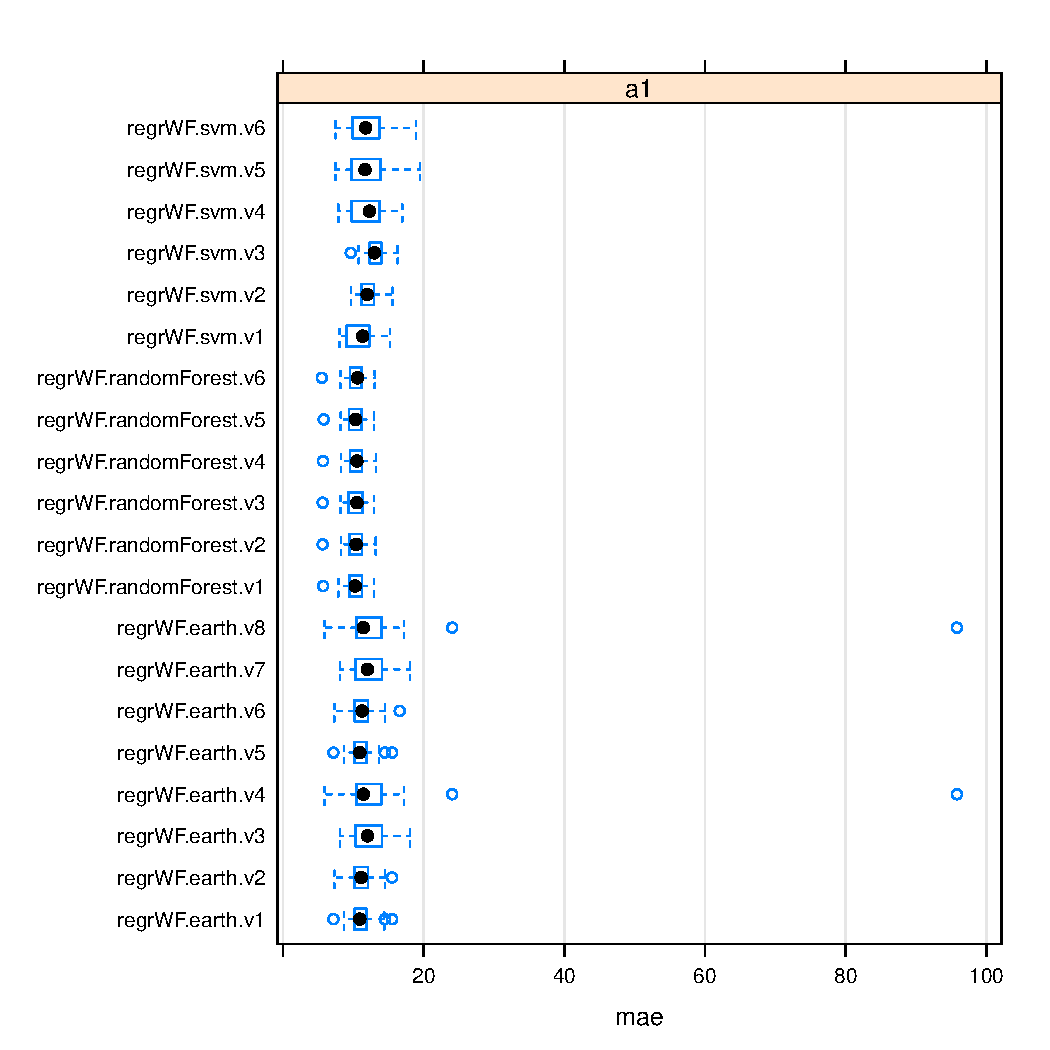
\includegraphics[width=\maxwidth]{figures/perfEst-unnamed-chunk-21} 

}



\end{knitrout}

  \caption{The MAE results for the task ``a1''.}
  \label{fig:maeA1}
\end{figure}

As before we are using the generic function \texttt{plot()} but this
time applied to a subset of the original object with all results. This
subset is obtained using the generic function \texttt{subset()} that
accepts several parameters to specify the subset we are interested
on. In this case we are using the parameters \texttt{dss} and
\texttt{stats} to indicate that we want to analyze only the results
concerning the task ``a1'' and the metric ``mae''. Other possibilities
are the parameters \texttt{vars} for indicating a subset of the
workflows, and \texttt{its} for indicating a subset of the
iterations. Both \texttt{vars}, \texttt{dss} and \texttt{stats} accept
as values a character string containing a regular expression that will
be used internally with the R function \texttt{grep()} over the vector
of names of the respective objects (names of the workflows, names of
the tasks and names of the metrics, respectively). For instance, if
you want to constrain the previous graph even further to the workflows
whose name ends in ``4'' (absurd example of course!), you could use
the following:

\begin{figure}[ht]
  \centering
\begin{knitrout}
\definecolor{shadecolor}{rgb}{0.969, 0.969, 0.969}\color{fgcolor}\begin{kframe}
\begin{alltt}
\hlkwd{plot}\hlstd{(}\hlkwd{subset}\hlstd{(res,} \hlkwc{dss} \hlstd{=} \hlstr{"a1"}\hlstd{,} \hlkwc{vars} \hlstd{=} \hlstr{"4$"}\hlstd{,} \hlkwc{stats} \hlstd{=} \hlstr{"mae"}\hlstd{))}
\end{alltt}
\end{kframe}

{\centering 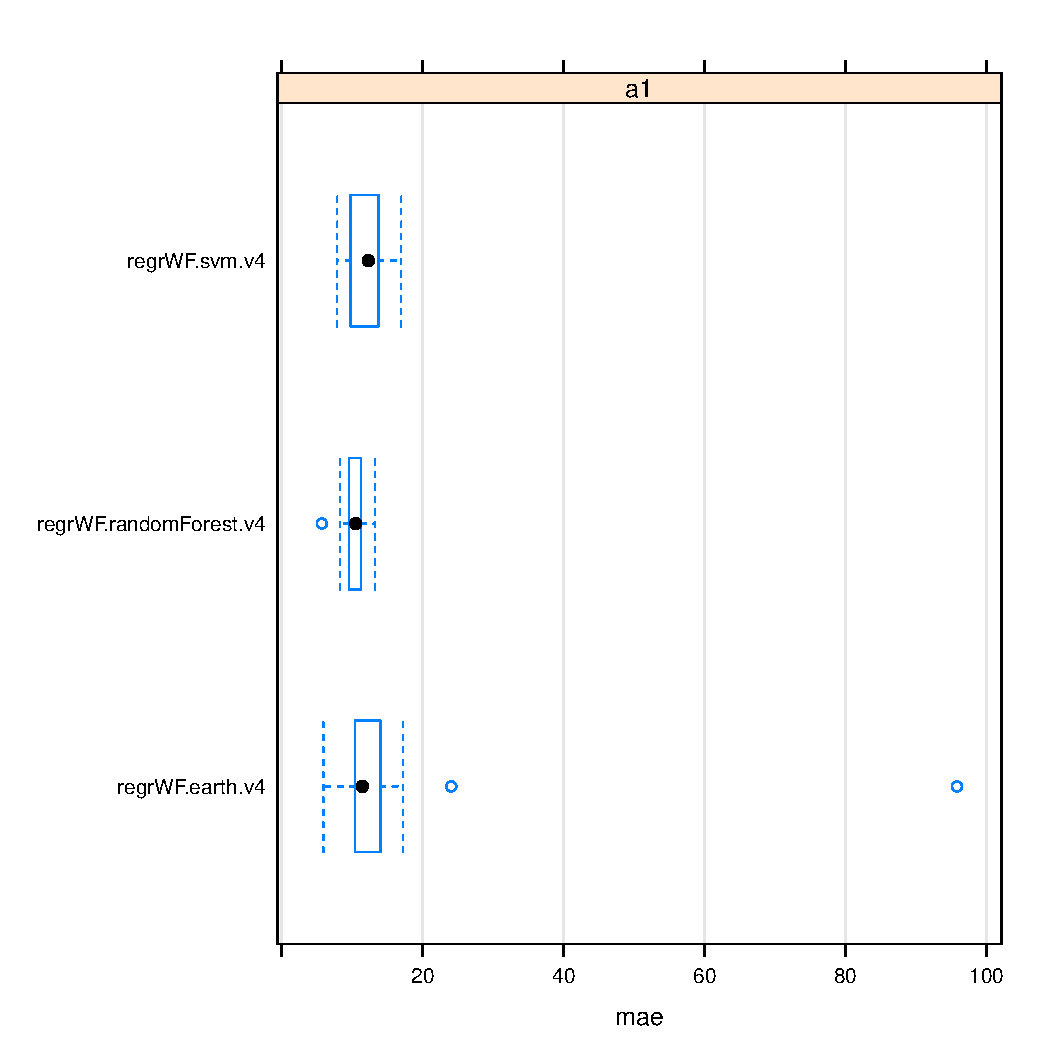
\includegraphics[width=\maxwidth]{figures/perfEst-unnamed-chunk-22} 

}



\end{knitrout}

  \caption{Illustration of the use of regular expressions in sub-setting the results objects.}
  \label{fig:maeA1b}
\end{figure}
%$

If you are more familiar with the syntax of "wildcards" you may use
the R function \texttt{glob2rx()} to convert to regular expressions,
as show in the following example:

\begin{knitrout}
\definecolor{shadecolor}{rgb}{0.969, 0.969, 0.969}\color{fgcolor}\begin{kframe}
\begin{alltt}
\hlkwd{summary}\hlstd{(}\hlkwd{subset}\hlstd{(res,} \hlkwc{dss} \hlstd{=} \hlstr{"a1"}\hlstd{,} \hlkwc{vars} \hlstd{=} \hlkwd{glob2rx}\hlstd{(}\hlstr{"*svm*"}\hlstd{),} \hlkwc{stat} \hlstd{=} \hlstr{"mae"}\hlstd{))}
\end{alltt}
\begin{verbatim}
## 
## == Summary of a  Cross Validation  Experiment ==
## 
##  3 x 10 - Fold Cross Validation run with seed =  1234 
## 
## * Data sets ::  a1
## * Learners  ::  regrWF.svm.v1, regrWF.svm.v2, regrWF.svm.v3, regrWF.svm.v4, regrWF.svm.v5, regrWF.svm.v6
## 
## * Summary of Experiment Results:
## 
## 
## -> Datataset:  a1 
## 
## 	*Learner: regrWF.svm.v1 
##            mae
## avg     11.119
## std      1.948
## min      8.032
## max     15.236
## invalid  0.000
## 
## 	*Learner: regrWF.svm.v2 
##            mae
## avg     12.080
## std      1.354
## min      9.649
## max     15.580
## invalid  0.000
## 
## 	*Learner: regrWF.svm.v3 
##            mae
## avg     13.018
## std      1.436
## min      9.639
## max     16.287
## invalid  0.000
## 
## 	*Learner: regrWF.svm.v4 
##            mae
## avg     12.008
## std      2.413
## min      7.878
## max     16.961
## invalid  0.000
## 
## 	*Learner: regrWF.svm.v5 
##            mae
## avg     11.839
## std      2.797
## min      7.479
## max     19.463
## invalid  0.000
## 
## 	*Learner: regrWF.svm.v6 
##            mae
## avg     11.947
## std      2.814
## min      7.453
## max     18.940
## invalid  0.000
\end{verbatim}
\end{kframe}
\end{knitrout}



The following are some illustrations of the use of other available
utility functions.

Obtaining the scores on all iterations and metrics of a workflow on a
particular data set:

\begin{knitrout}
\definecolor{shadecolor}{rgb}{0.969, 0.969, 0.969}\color{fgcolor}\begin{kframe}
\begin{alltt}
\hlkwd{getFoldsResults}\hlstd{(res,} \hlstr{"regrWF.svm.v6"}\hlstd{,} \hlstr{"a3"}\hlstd{)}
\end{alltt}
\begin{verbatim}
##      mae     mse
## 1  3.738  35.167
## 2  5.720  85.866
## 3  3.062  24.207
## 4  4.421  58.519
## 5  6.916 161.427
## 6  3.818  43.422
## 7  5.972  77.363
## 8  2.989  13.756
## 9  3.522  31.301
## 10 4.421  31.060
## 11 7.058  98.894
## 12 3.984  34.912
## 13 3.358  28.457
## 14 4.479  51.942
## 15 5.356 120.784
## 16 3.115  18.346
## 17 5.057  67.551
## 18 4.645  78.109
## 19 3.866  37.893
## 20 3.021  23.811
## 21 2.573  12.475
## 22 3.327  32.153
## 23 2.284   8.395
## 24 5.643  72.897
## 25 3.699  35.598
## 26 5.157  73.571
## 27 5.329 116.683
## 28 4.154  68.635
## 29 4.765  49.770
## 30 4.611  57.290
\end{verbatim}
\end{kframe}
\end{knitrout}


Getting the summary of the results of a particular workflow on a  data set :

\begin{knitrout}
\definecolor{shadecolor}{rgb}{0.969, 0.969, 0.969}\color{fgcolor}\begin{kframe}
\begin{alltt}
\hlkwd{getSummaryResults}\hlstd{(res,} \hlstr{"regrWF.svm.v3"}\hlstd{,} \hlstr{"a7"}\hlstd{)}
\end{alltt}
\begin{verbatim}
##           mae     mse
## avg     3.060  28.632
## std     1.062  25.950
## min     1.462   4.234
## max     6.196 110.198
## invalid 0.000   0.000
\end{verbatim}
\end{kframe}
\end{knitrout}


Finally, the \texttt{statScores()} function allows you to apply any
summary function (defaulting to \texttt{mean()}) to the results on a
certain statistic given in parameter \texttt{stat}. The following
calculates the median of the results of the SVMs on the task ``a1'',

\begin{knitrout}
\definecolor{shadecolor}{rgb}{0.969, 0.969, 0.969}\color{fgcolor}\begin{kframe}
\begin{alltt}
\hlkwd{statScores}\hlstd{(}\hlkwd{subset}\hlstd{(res,} \hlkwc{vars} \hlstd{=} \hlkwd{glob2rx}\hlstd{(}\hlstr{"*svm*"}\hlstd{),} \hlkwc{dss} \hlstd{=} \hlstr{"a1"}\hlstd{),} \hlkwc{stat} \hlstd{=} \hlstr{"mae"}\hlstd{,} \hlkwc{summary} \hlstd{=} \hlstr{"median"}\hlstd{)}
\end{alltt}
\begin{verbatim}
## $a1
## regrWF.svm.v1 regrWF.svm.v2 regrWF.svm.v3 regrWF.svm.v4 regrWF.svm.v5 regrWF.svm.v6 
##         11.34         11.97         12.99         12.30         11.66         11.76
\end{verbatim}
\end{kframe}
\end{knitrout}

%\section{Conclusions}

\bibliographystyle{alpha}
\bibliography{compExps}
\end{document}
